\documentclass[a4paper]{article}
\usepackage{amsmath, bm, amssymb, hyperref, parskip, graphicx, tikz, subcaption, wrapfig, mathtools, placeins}
\usepackage{multicol, enumitem, rotating}
\usepackage[round]{natbib}
\usepackage[margin=1.2in]{geometry}
\bibliographystyle{plainnat}

%\renewcommand*{\bibfont}{\interlinepenalty 10000\relax}

\usetikzlibrary{hobby}

\graphicspath{{./figs/}}

\title{\bf Penetration of convective plumes into a stably stratified layer: turbulent mixing \& tracer
	transport}
\author{Charles Powell}

\begin{document}
\maketitle

\begin{abstract}
	Intense thunderstorms in the equatorial lower atmosphere can occasionally overshoot into the stratosphere,
	carrying small amounts of water vapour with them and irreversibly hydrating the surrounding environment.
	As one of the primary possible pathways for vertical transport of water vapour into the middle atmospheric
	layer, it is important to understand and quantify the processes resulting in irreversible transport. We
	reduce the problem to understanding the mixing that occurs as a convective plume of fluid penetrates a
	stable layer, emulating the atmospheric setup.  By neglecting complicating factors such as the large-scale
	atmospheric flow, intra-cloud processes and thermodynamics, the essential mechanisms are more easily
	studied and interpreted. In this essay we explore the dynamics of the turbulent flow in a fluid plume
	rising from a source of buoyancy, first in a uniform environment, then with the introduction of a
	stratified layer in which the fluid density decreases linearly with height. The central questions of this
	problem are how much tracer is carried to regions with active mixing between the plume and environment,
	how much actually mixes with the environment, and how much tracer therefore remains in the stable layer?
	To that end, we explore the distribution of tracer across fluid elements with a range of buoyancy, in
	particular presenting a method of distinguishing volumes of plume fluid which have mixed with the
	environment from those which have not. We also discuss methods of visualising and characterising the
	turbulent mixing between the plume and environmental fluid, focussing on metrics which quantify the
	intensity and efficiency of mixing. Finally, we discuss possible routes from the aforementioned analyses
	to a quantitative model applicable to the original atmospheric problem.
\end{abstract}

%%%%%%%%%%%%%%%%%%%%%%%%%%%%%%%%%%%%%%%%%%%%%%%%%%%%%%%%%%%%%%%%%%%%%%%%%%%%%%%%%%%%%%%%%%%%%%%%%%%%%%%%%%%%%

\section{Introduction}

In the tropical upper troposphere and lower stratosphere (UTLS), convective plumes generated by strong
thunderstorm complexes can penetrate through the tropical tropopause layer (TTL) into the lower stratosphere.
Stratospheric composition is largely set by cross-tropopause transport in the tropics as tropospheric air
predominantly enters the stratosphere in the tropics \citep{fueglistaler2009}. There is an ongoing debate on
the importance of convective penetration in this transport, particularly with respect to water vapour, where
it may allow the local temperature constraint on concentrations to be avoided and lead to a hydrating effect
\citep{jensen2007}. There exists numerical simulations of convective penetration events in complex
meteorological models \citep{dauhut2015, dauhut2018} containing many physical processes but this is
computationally expensive and more challenging to interpret. In this project, the working hypothesis is that
the process of convective penetration in the UTLS itself can be greatly simplified by considering a simple
fluid dynamical problem representative of the TTL, in which a region of strong stable stratification is
penetrated by a turbulent buoyant plume generated in a region with weak or zero stable stratification.

We neglect many complicating factors such as shear in the strongly stably stratified layer, the thermodynamics
of distinct phases of water, and associated latent heating in favour of a passive tracer and a quiescent
environment. The simplified nature of the problem is expected to make investigation of passive tracer
transport and mixing clearer and aid the development of models of this transport as a function of
characteristic plume quantities. The effect of complicating factors on transport can then be considered later,
by directly introducing shear, or via simple parameterisations of thermodynamic effects such as saturation and
sublimation using multiple tracers. Further, the fluid dynamical problem of convective penetration itself is of continuing scientific
interest in the literature, in particular the generation of gravity waves by the penetrating plume cap and the
energetics of the system, with applications to many problems. It has only recently become possible to
numerically simulate this problem at mid to high resolution, owing to constraints such as the domain size
needed to control edge effects, among others.

In this essay we focus on developing methods of analysing the turbulent mixing and the
associated passive tracer transport, rather than presenting results on the dependence of these processes on the
stratification strength, which will be the immediate focus of our future work. Here, we work towards a general
picture of the mixing characteristics in convective penetration, so that we may understand what changes when
stratification strength is modified. First, we explore the dynamics of a
buoyant plume in an unstratified environment, then with a linearly stably stratified environment overlying an
unstratified layer of fixed depth where the plume is generated. We then consider methods of visualising the
tracer distribution in buoyancy space and identify the changes that result from mixing between the plume and
environment. A method of identifying plume fluid which has mixed with the environment is developed, by
extending the buoyancy-tracer joint PDF utilised in \citet{penney2020} with a correction for the buoyancy-tracer
distribution which enters the control volume and utilising transport properties of mixing and stirring in
buoyancy-tracer space. This is the central result of this essay; the segregated volume distribution
allows consideration of the changing characteristics of plume fluid before and after mixing with the
environment (which we will refer to as pre- and post-mixed), and provides a basis for comparing the
penetration problem under varied stratification strength. We then discuss the characteristics of pre- and
post-mixed fluid in the context of metrics which quantify the intensity, efficiency and mechanism of mixing,
demonstrating a way to exploit the segregated volume distribution method. Finally, we briefly discuss ideas
which will take the research presented in this essay further.

%%%%%%%%%%%%%%%%%%%%%%%%%%%%%%%%%%%%%%%%%%%%%%%%%%%%%%%%%%%%%%%%%%%%%%%%%%%%%%%%%%%%%%%%%%%%%%%%%%%%%%%%%%%%%

\section{Unstratified plume dynamics}

In this section we explore the canonical theory for the dynamics of a plume in an unstratified environment. We
then detail the numerical methods used for simulating such a plume, and use the results of one of these high
resolution simulations to understand the turbulent dynamics of a simple buoyant plume. This provides a basis
for understanding the essential physics of a turbulent plume which we will use throughout the remainder of
this essay. 

\subsection{Canonical plume theory}

A buoyant plume is the shear-free flow resulting from a localised and continuous source of buoyancy. A
`forced' plume has non-zero source momentum whilst a `pure' plume has none. The
canonical theory of plumes pioneered by \citet{mtt} (henceforth MTT) is centred on a
self-similarity hypothesis: far from the source and ignoring molecular effects, velocity
and buoyancy collapse onto a single profile when normalised by characteristic scales $r_m, w_m, b_m$.
These scales are defined with respect to the integral buoyancy flux, momentum flux, and volume flux $F, M, Q$
associated with the plume, as well as the integral buoyancy $B$, collectively referred to as integral
quantities. We have
\begin{equation}
	r_m \equiv \frac{Q}{M^{1/2}}, \hspace{1em} w_m \equiv \frac{M}{Q}, \hspace{1em} b_m \equiv \frac{BM}{Q^2} =
	\frac{B}{r_m^2} = \frac{F}{\theta_m Q}
\end{equation}
where 
\begin{equation}
	Q \equiv 2\int_0^\infty \overline{w}r \, \mathrm{d}r, \hspace{1em} M \equiv 2\int_0^\infty \overline{w}^2
	r\, \mathrm{d}r, \hspace{1em} B \equiv 2 \int_0^\infty \overline{b}r\,\mathrm{d}r, \hspace{1em} F \equiv
	\int_0^\infty \overline{w}\overline{b}r\,\mathrm{d}r
	\label{eq:intquant}
\end{equation}
These integral quantities naturally arise from radially integrating the Boussinesq equations for conservation
of mass, momentum, buoyancy and energy. The resulting equations govern the vertical evolution of these fluxes:
\begin{align}
		\frac{\mathrm{d}Q}{\mathrm{d}z} &= 2\alpha M^{1/2} \label{eq:plume1}\\ 
		\frac{\mathrm{d}}{\mathrm{d}z}\left(\beta_g M \right) &= \frac{FQ}{\theta_m M} \label{eq:plume2}\\
		\frac{\mathrm{d}}{\mathrm{d}z}\left(\frac{\theta_g}{\theta_m} F\right) &= -N^2 Q\label{eq:plume3} \\ 
		\frac{\mathrm{d}}{\mathrm{d}z}\left(\gamma_g\frac{M^2}{Q}\right) &= 2F + \delta_g \frac{M^{5/2}}{Q^2}
		\label{eq:plume4}
\end{align}
Here, $N^2$ is the buoyancy frequency associated with the ambient fluid and $\alpha$ is the entrainment
coefficient, arising from the hypothesis $-\left[ru\right]_{r=\infty} = \alpha r_m w_m$ made by MTT which says
that the inward radial volume flux is proportional to the vertical volume flux in the plume. The
remaining parameters $\beta, \theta, \delta, \gamma$ are profile coefficients describing the relative shape of
the self-similar profiles and are a more modern development. Note that equations
\eqref{eq:plume1}--\eqref{eq:plume4} are consistent with both top-hat and Gaussian radial profiles, but
inconsistent with the MTT assumption that profiles of different variables share the same width.

The above theory provides a basis for examining simulations of turbulent plumes. The PhD thesis of
\citet{craske} and associated papers (e.g.\ \citet{mvr2016}, henceforth VR16) consider direct numerical
simulation of a turbulent jet, forced plume and pure plume in a 3D domain with open boundaries and a
homogeneous environment.  They use the integral theory of MTT, with the turbulent corrections provided by
profile coefficients, to examine the turbulent dynamics and entrainment properties in each flow. Following
their work, we process the results of numerical simulations by performing an azimuthal average to separate the
mean and turbulent components. Note that in theory, these averages are over the semi-infinite domain $r>0$ but
clearly a simulation has a finite domain. We minimise the error associated with finite domain approximations
of integrals over an infinite radial domain via `thresholding', which places the upper limit of the integral
at the first point where the vertical velocity reaches a small fraction of its value on the centreline.

\subsection{Simulation methods}
\label{sec:setup}

Numerical simulation of the plume penetration problem offers some potential advantages over laboratory
experiments; for instance, it is straightforward to include complicating factors such as large-scale
horizontal flow, or simple representations of physical effects, as well as providing access to full 3D
dynamical fields which may be used for analysing the flow. For this work, we use the Fortran codebase
`DIABLO'. DIABLO evolves a discrete approximation of the Navier-Stokes equations \eqref{eq:ns1},
\eqref{eq:ns2} and buoyancy evolution equation \eqref{eq:ns3} using a pseudo-spectral method in the horizontal
with periodic boundary conditions and finite difference in the vertical with fixed wall boundaries. Owing to
the large range of scales in the UTLS, resolving turbulent scales with direct numerical simulation would incur
a great computational cost. We therefore use large eddy simulation (LES) with the anisotropic minimum
dissipation (AMD) eddy-viscosity model for capturing the dynamic effects of unresolved scales
\citep{taylor2018}. The dimensional governing equations are
\begin{align}
		\frac{\partial \widehat{u}_i}{\partial x_i} &= 0 \label{eq:ns1}\\
	\frac{\mathrm{D} \widehat{u}_i}{\mathrm{D}t} + \frac{\partial \widehat{p}}{\partial x_i} &= \nu \frac{\partial^2
		\widehat{u}_i}{\partial x_j \partial x_j} + \widehat{b}\delta_{i3} - \frac{\partial \tau_{ij}}{\partial x_j}
		\label{eq:ns2}\\
		\frac{\mathrm{D}\widehat{b}}{\mathrm{D}t} &= \kappa_b \frac{\partial^2 \widehat{b}}{\partial x_j \partial x_j}
		- \frac{\partial \lambda_j}{\partial x_j} \label{eq:ns3}
\end{align}
where $\widehat{\cdot}$ indicates filtering at the resolved grid scale, $\delta_{ij}$ is the delta function,
$\nu$ is the kinematic viscosity, $\kappa_b$ is the diffusivity of buoyancy $b = -g\rho'/\rho_0$,
the sub-grid-scale (SGS) stress is $\tau_{ij} = \widehat{u_i u_j} - \widehat{u}_i \widehat{u}_j$ and the SGS
buoyancy flux is $\lambda_j = \widehat{u_i b} - \widehat{u}_i \widehat{b}$. The eddy-viscosity model for the
deviatoric component of the SGS stress and the SGS buoyancy flux are
\begin{equation}
	\tau_{ij}^d = \tau_{ij} - \frac{1}{3}\delta_{ij}\tau_{kk} = -2\nu_T \widehat{S}_{ij}, \hspace{2em} \lambda_j =
	-\kappa_{b,T} \frac{\partial \widehat{b}}{\partial x_j}
\end{equation}
where $\nu_T$ and $\kappa_{b,T}$ are the turbulent eddy viscosity and eddy diffusivity respectively, each
determined by the AMD scheme. The hat notation is now dropped for convenience.

For simulating plumes, we may non-dimensionalise via the source radius $r_0$ and the integral source buoyancy
flux $F_0 = r_0^2 w_0 b_0$ with $\left[F_0\right] = L^4 T^{-3}$, leaving two characteristic numbers
$\mathrm{Re} \equiv (F_0r_0^2)^{1/3}/\nu$ and $\mathrm{Pr} \equiv \nu /\kappa$. The intrinsic velocity scale
is $U \sim F_0^{1/3} r_0^{-1/3}$ and the intrinsic timescale is $T \sim r_0^{4/3} F_0^{-1/3} \equiv r_0/U$
known as the \emph{turnover time}, interpreted as the time for an eddy to become significantly distorted
\citep{frisch1995}. In this initial verification work, the background buoyancy profile is unstratified for
simplicity, but later we impose a linear stratification on the background profile. A buoyant plume is
generated using a volumetric forcing method in which the buoyancy and vertical velocity are relaxed towards
prescribed analytic profiles for a pure plume, derived from the MTT equations
\eqref{eq:plume1}--\eqref{eq:plume3}, in a thin region at the bottom of the domain. A random 10\% perturbation
is applied to the profile in the forcing region and to the velocity in the two grid layers above the forcing
region to initiate turbulence. The forcing region is set by two parameters $L_c$ and $L_p$ which control a
$\tanh$ function modulating the prescribed profiles. To illustrate, given vertical profiles $r_m(z), b_m(z)$
consistent with the desired plume, the forcing applied to $b$ (excluding random perturbations) is
\begin{align}
	f_b(\bm{x}) &= \left(b(\bm{x}) -
		2b_m(z)\exp\left[-\frac{1}{2}\frac{x^2+y^2}{r_m(z)^2}\right]\right)\left(\frac{1}{2}-\frac{1}{2}\tanh\left(\frac{z-L_c}{L_p}\right)\right)
\end{align}
The first factor is the difference between the dynamical buoyancy field and the prescribed buoyancy (assuming
a Gaussian radial profile), whilst the second factor limits the forcing to $0 \le z \lessapprox L_c + L_p$.
The parameter $L_c$ approximately controls the depth of the forcing region and $L_p$ determines how sharply
the forcing decays above $z=L_c$. The forcing region is indicated in figure~\ref{fig:radius}. A parameter
$1/\tau$ controls the coupling strength with the momentum equations. The size of $\tau$ is arbitrary other
than being small enough to control against dynamical variation and large enough to prevent numerical
instability.

In the remainder of this section, all data is from a high resolution LES simulation with grid size $N_x
\times N_y \times N_z = 1024 \times 1024 \times 1025$, dimensional size $L_x = L_y = \frac{1}{2}L_z = 50r_0$,
source radius $r_0 = 10 \,\mathrm{m}$ and source buoyancy flux $F_0 = 0.08r_0^2 \,m^4 s^{-3}$. For the
unstratified plume, simulations are first run until the plume is fully developed and `statistically steady',
which is verified by ensuring buoyancy and vertical velocity exhibit self-similar profiles and the running
time average with $n$ timesteps of each variable is sufficiently steady. The number of observations $n$ must be
large enough that the total time over which samples are averaged is greater than the intrinsic timescale $T$
of the flow. The simulation is then run in data-collection mode for approximately $100$ turnover times. For a
discussion of the azimuthal averaging \& Reynolds' decomposition method and limitations of this simulation
setup, see appendix~\ref{app:postprocessing} and~\ref{app:limitations} respectively.

\subsection{Integral quantities, self-similarity and entrainment}

\begin{figure}
	\centering
	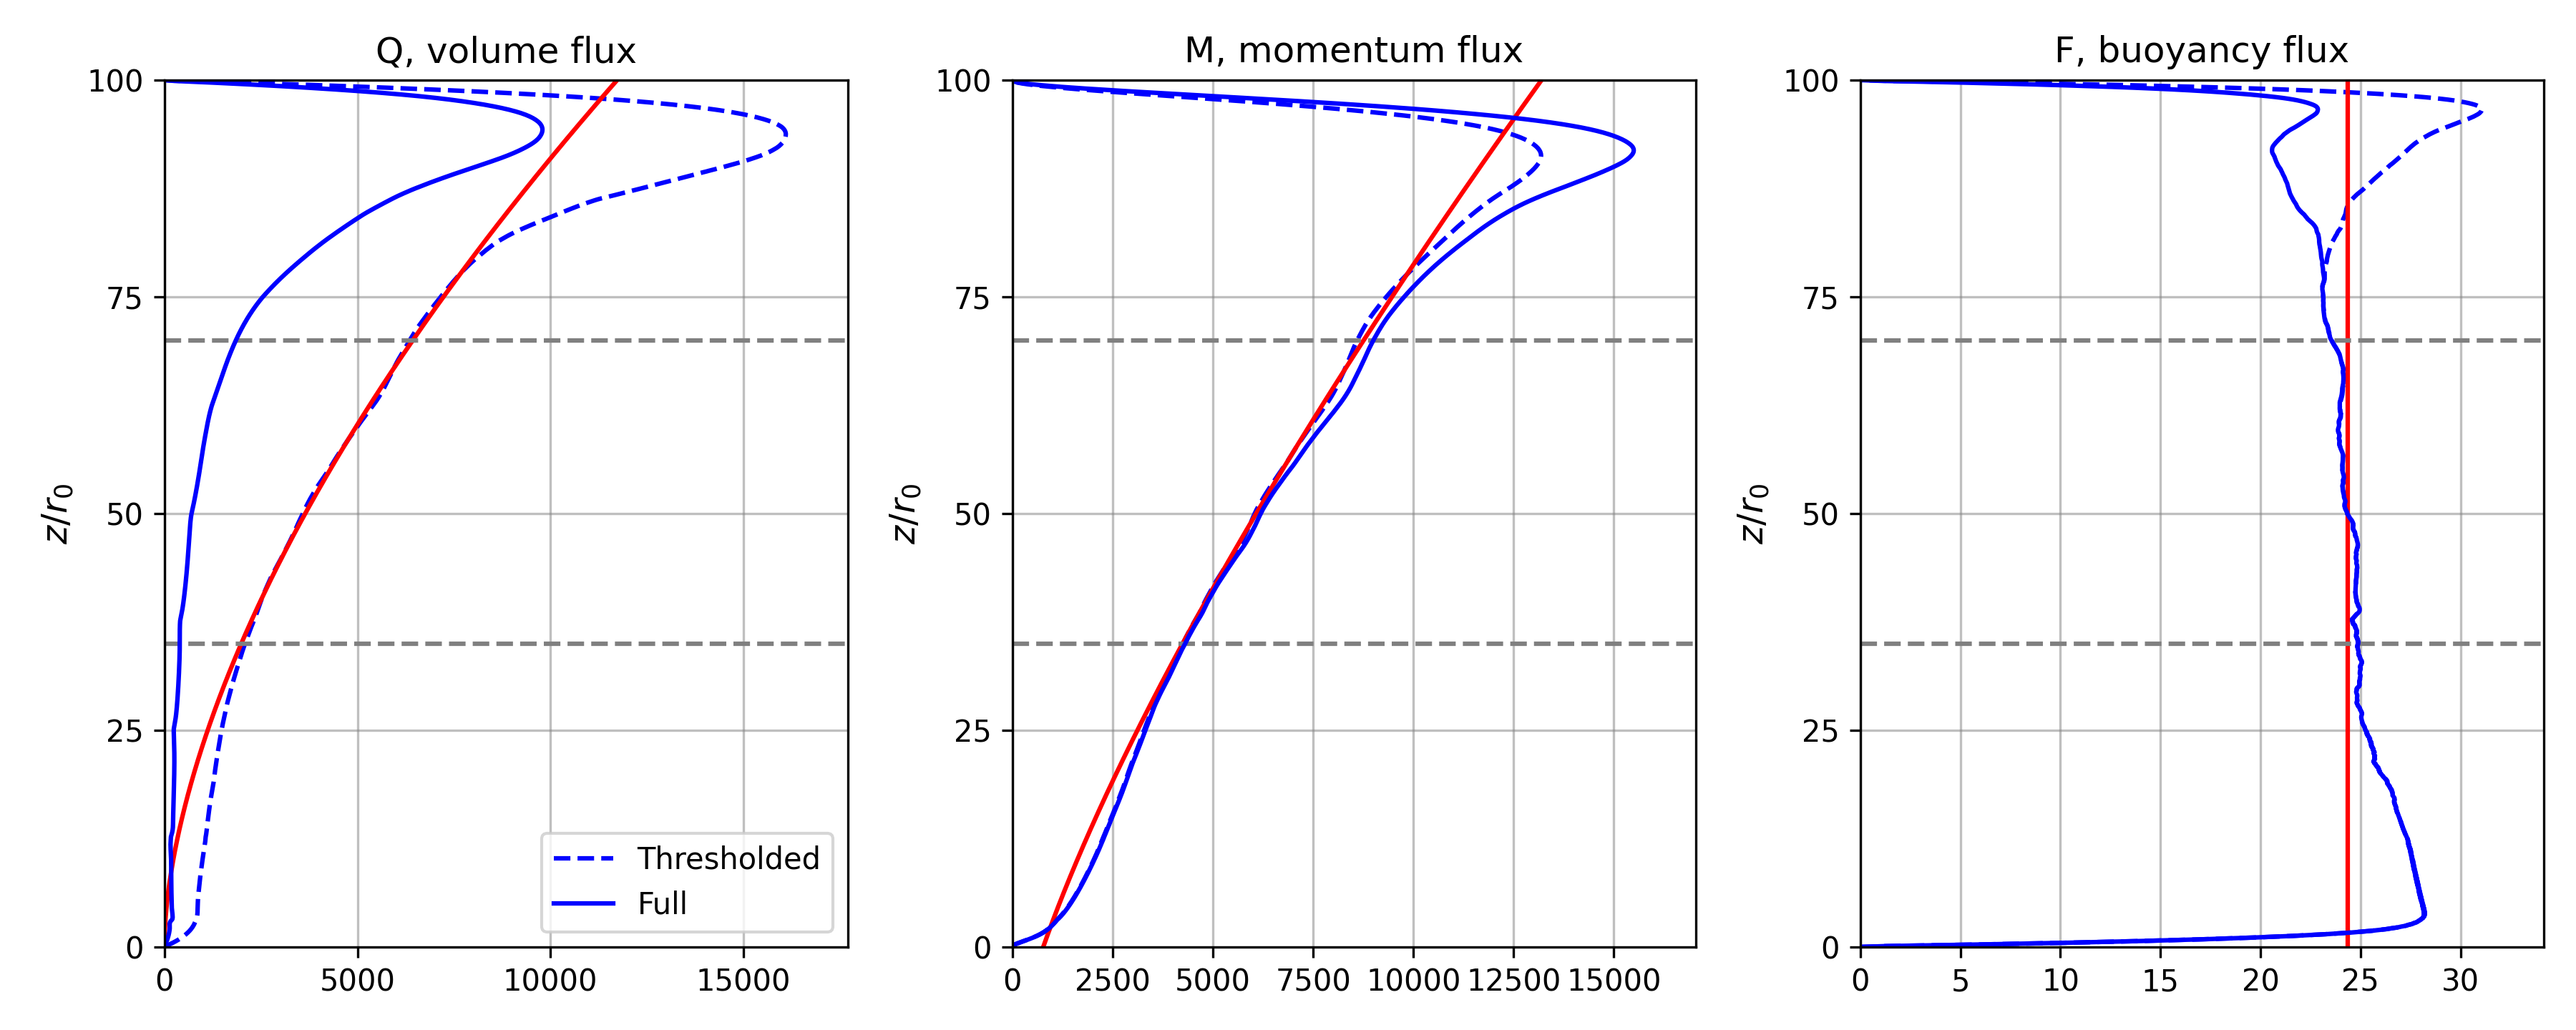
\includegraphics[width=.8\textwidth]{mvr/fig0.png}
	\caption{Variation of integral quantities $Q, M, F$ defined by \eqref{eq:intquant} with height $z$.
	Results from simulation described in section~\ref{sec:setup} with
	$w$-based thresholding shown in dashed blue and the original (full) integral quantities shown in blue.
	MTT analytic predictions fitted to the simulation data shown in red. Dashed grey lines indicate the
	region used to fit the analytic curves.}
	\label{fig:QMF}
\end{figure}

In the integral formulation, the plume dynamics are fully determined by $r_m, w_m$ and $b_m$, which in turn
are fully determined by the vertical evolution of integral quantities $Q, M$ and $F$. Figure~\ref{fig:QMF}
shows the variation of these quantities with height (streamwise distance) $z$. Following the methods of
\citet{craske}, we calculate infinite radial integrals by thresholding the domain at the radius where vertical
velocity $\overline{w}$ falls below a specified ratio $\varepsilon$ of the centreline vertical velocity. The
thresholded data is of particular interest as it represents the fluxes contained within the plume, excluding
the surrounding environment. The integral formulation of the plume equations
\eqref{eq:plume1}--\eqref{eq:plume3} admit power-law solutions with scalings $Q \sim z^{5/3}, M \sim z^{4/3}$
and $F \sim \text{const}$. Curves of this form are shown in figure~\ref{fig:QMF} and demonstrate a good fit
with the thresholded integral fluxes. 
\begin{figure}
	\centering
	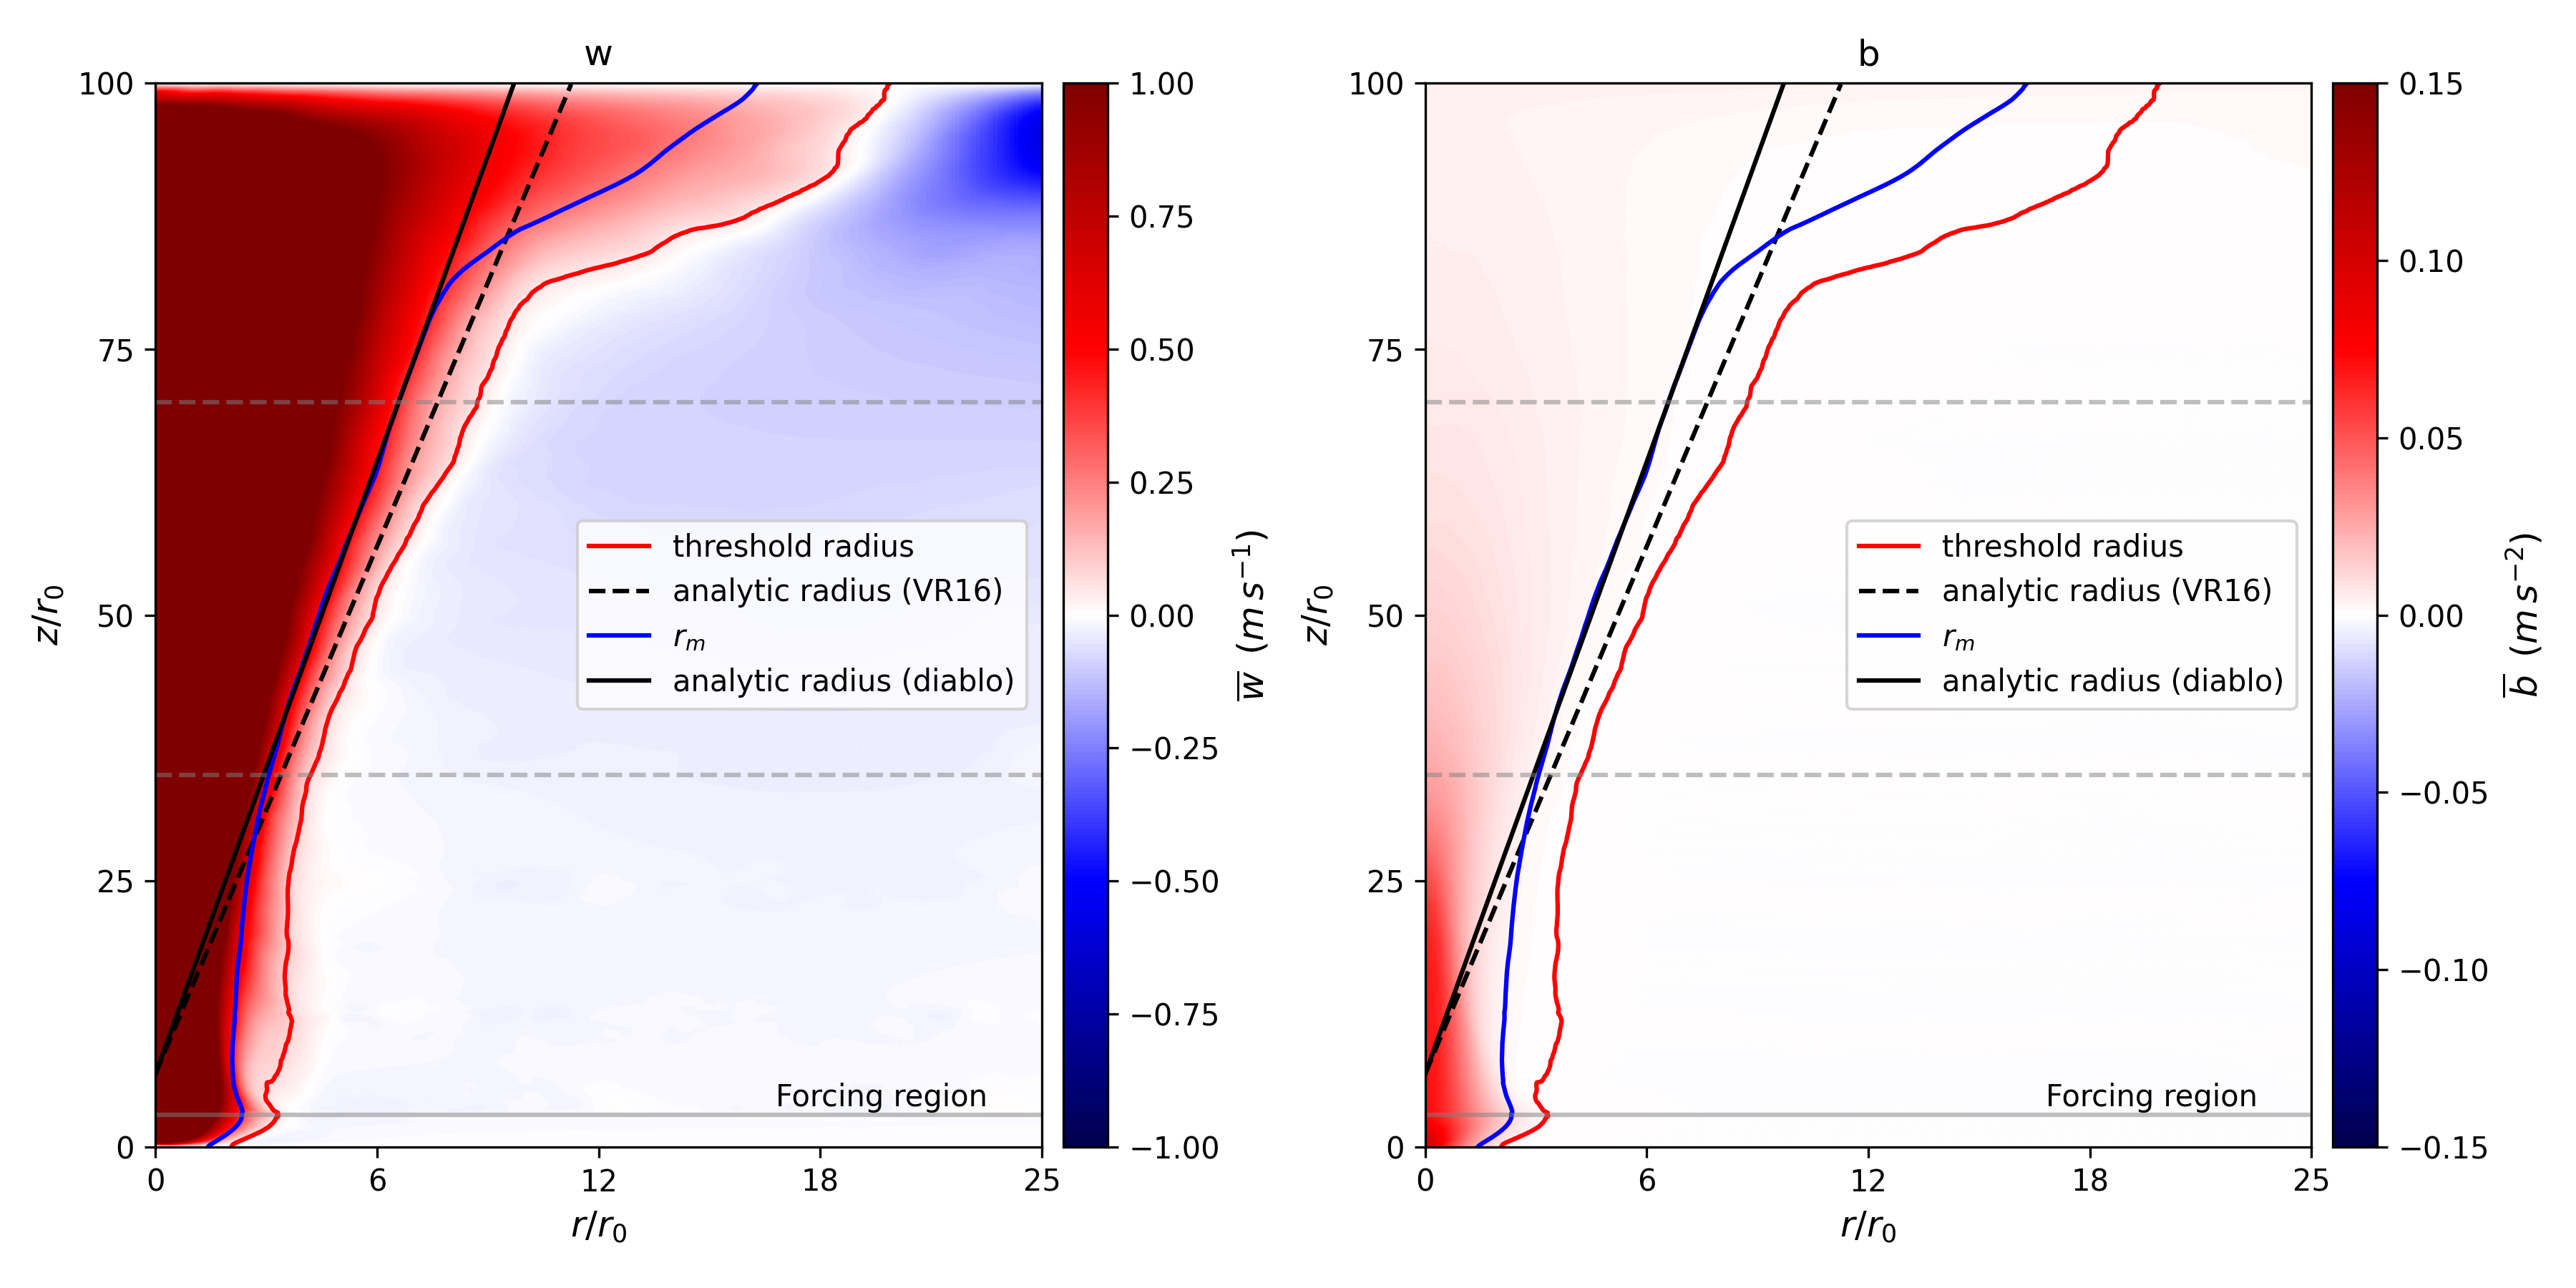
\includegraphics[width=.8\textwidth]{mvr/fig7.png}
	\caption{Azimuthally \& ensemble averaged vertical velocity $w$ (left) and buoyancy $b$ (right). Variation
	of characteristic plume radius $r_m(z)$, analytic radius from DIABLO simulations, analytic radius from
	VR16 simulations, and threshold radius used for computing radial integrals are overlaid.}
	\label{fig:radius}
\end{figure}

Figure~\ref{fig:radius} shows the azimuthally averaged vertical velocity and buoyancy fields. The
buoyant plume appears as a region of strong vertical velocity localised to small radii. The linear increase
of plume radius with height as predicted by MTT theory is evident. The dashed black line shows the
analytic radius $r_m$ (calculated from the power-law solutions for $M$ and $Q$) as a function of height using
the value of the entrainment coefficient found in VR16 direct numerical simulations, $\alpha = 0.105$. The
solid black line uses the entrainment coefficient resulting from our large eddy simulations, $\alpha = 0.09$,
which demonstrates slightly weaker entrainment in our simulations, but still within the range of $\alpha$
found in the literature. The figure also demonstrates that only the middle third of the domain is suitable for
analysis; the forcing region at the bottom of the domain, in which the vertical velocity and buoyancy are
forced, underlies an adjustment region in the bottom third of the domain where source effects gradually decay.
In the top third of the domain where the plume impinges on the closed top boundary and spreads laterally, a
weak stratification is gradually introduced which inhibits the rise of the plume.

\begin{figure}
	\centering
	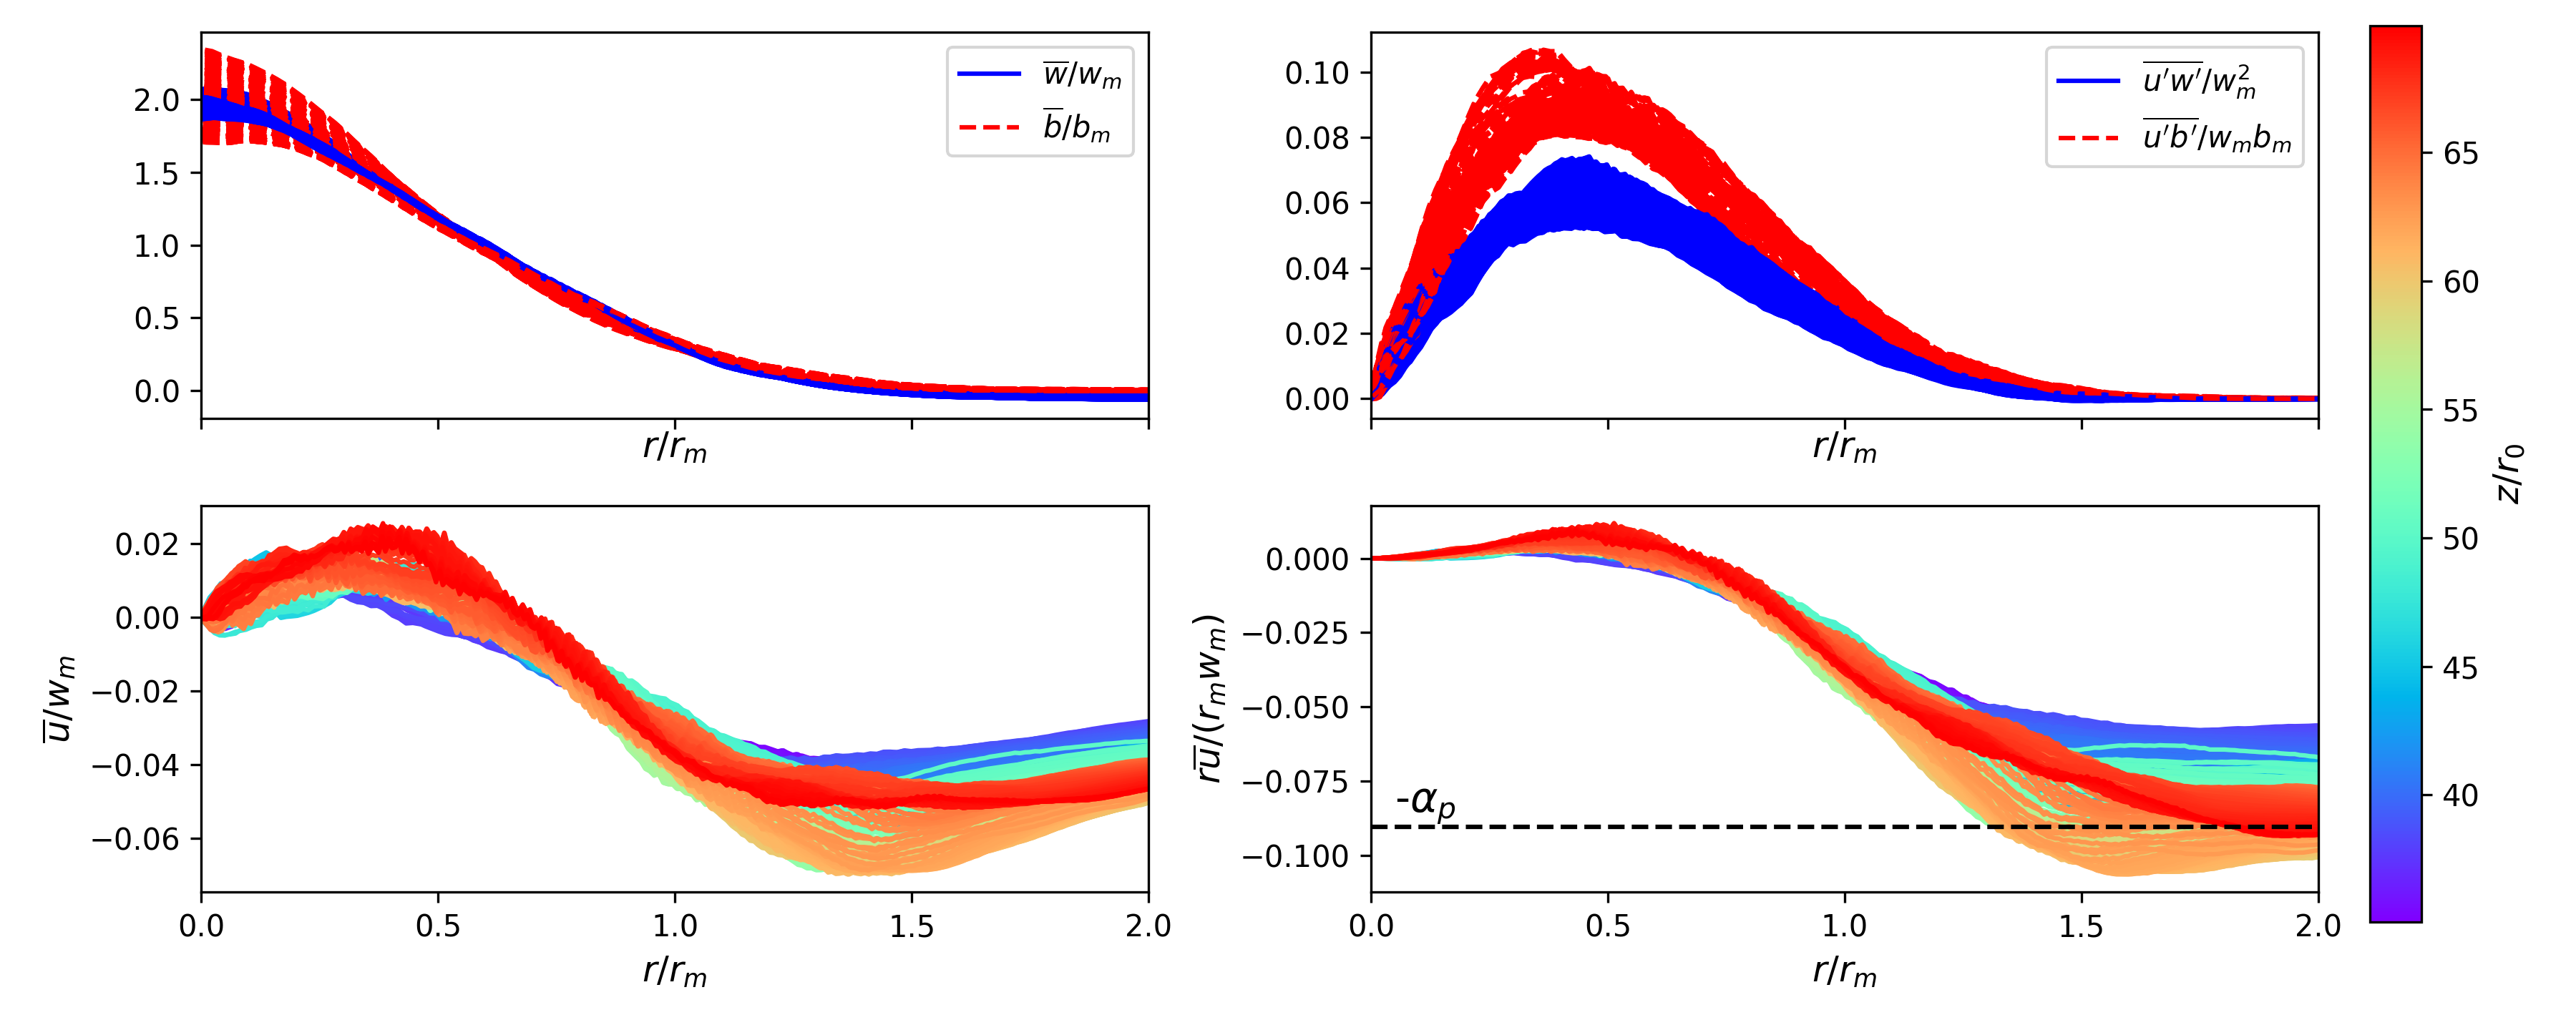
\includegraphics[width=\textwidth]{mvr/fig23}
	\caption{Self-similar radial profiles of $\overline{w}, \overline{b}$ (top left), radial momentum and
		buoyancy fluxes $\overline{u'w'}$ and $\overline{u'b'}$ (top right), mean radial velocity
		$\overline{u}$ (bottom left) and normalised mean radial specific volume flux $r\overline{u}$ (bottom
		right) in the interval $35 < z/r_0 < 70$. Dotted line indicates value of $\alpha_p$ calculated from a
		linear fit of $r_m$ and $z$.}
	\label{fig:selfsimilarradial}
\end{figure}

Self-similarity is one of the central ideas of MTT theory. The vertical velocity, buoyancy, radial momentum and
buoyancy flux profiles over a range of streamwise heights $z$ are shown normalised by the characteristic
scales $r_m, b_m, w_m$ at each height in figure~\ref{fig:selfsimilarradial}, demonstrating convergence to a
single radial profile. This is a useful diagnostic for future simulations; self-similar profiles indicate
that the plume is fully developed. Figure~\ref{fig:selfsimilarradial} also shows the normalised radial
velocity and specific volume flux. Whilst they are approximately self-similar, there is more spread than the
$\overline{w}, \overline{b}$-profiles, likely due to the periodic (i.e.\ effectively closed) boundaries as
compared with the open boundaries of VR16. In our case, the periodic boundaries result in an overturning
circulation which disrupts the radial outflow from the plume. Nonetheless, the radial specific volume flux
tends towards $-\alpha$ as $r/r_m$ increases which verifies the entrainment hypothesis and demonstrates that
plume entrainment is behaving broadly as expected. 

Figure~\ref{fig:entrain} shows the vertical evolution of the entrainment coefficient, calculated directly from
the MTT equations which give $\alpha = (2M^{1/2})^{-1}dQ/dz$. The value calculated from a linear fit of the
characteristic plume radius $r_m$ to $z$ is shown by a black vertical line $\alpha_p$. Whilst there is
significant variation, in the middle third of the domain suitable for analysis $\alpha$ lies within a narrower
band $0.06 < \alpha < 0.1$, again within the range found in the literature. The flux balance parameter
$\Gamma$ is also shown in figure~\ref{fig:entrain}. This is a normalised Richardson number, defined as

\begin{equation}
	\Gamma = \frac{5FQ^2}{8\alpha_p \beta_g \theta_m M^{5/2}}
	\label{eq:rich}
\end{equation}

indicating the balance of gravitational and inertial forcing. A `pure' plume has $\Gamma = 1$, a `lazy' plume
$\Gamma > 1$, a `forced' plume $0 < \Gamma < 1$ and a jet has $\Gamma = 0$. In our simulations, away from the
source $\Gamma \approx 0.5$ indicating a forced plume in which buoyancy dominates, but with inertial forcing
present. Whilst our simulations use forcing conditions for a pure plume, it is clear from comparison with VR16
that our results more closely match those of a forced plume, since our volumetric forcing method involves
relaxing the vertical velocity which introduces some inertial forcing. This illustrates the difficulty of
balancing the inertial and buoyancy forcing to obtain a pure plume, which is often cited as a reason for
simulating forced plumes or jets instead. Since pure plumes and jets are special cases where $\Gamma$ takes a
single value, a forced plume can be considered the more general case. We anticipate that a forced plume is
therefore more representative of the atmospheric case.

\begin{figure}
	\centering
	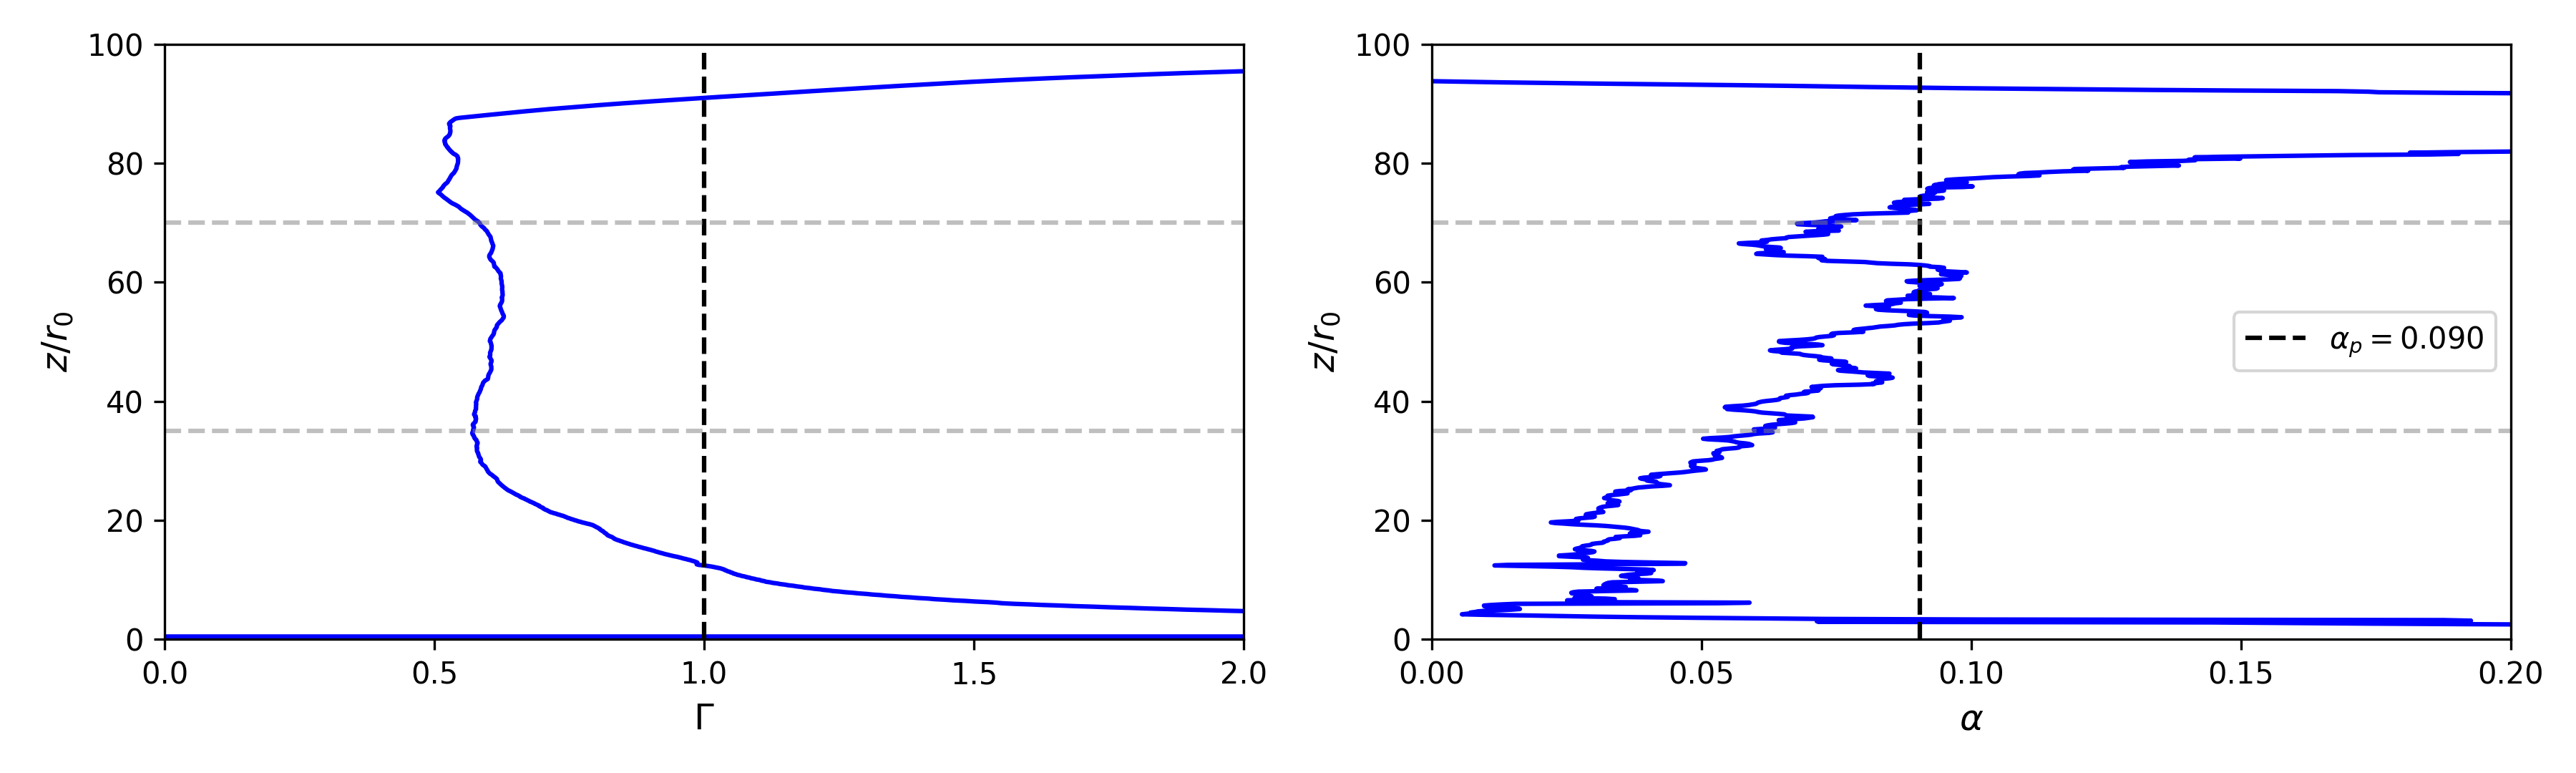
\includegraphics[width=\textwidth]{mvr/fig8}
	\caption{Vertical evolution of the flux balance parameter $\Gamma$ and the entrainment coefficient
	$\alpha = (2M^{1/2})^{-1} \mathrm{d}_z Q$}
	\label{fig:entrain}
\end{figure}

\subsection{Profile coefficients and turbulence characteristics}
Profile coefficients are a modern addendum to the MTT plume equations which, in a radially averaged sense,
account for the (non-dimensionalised) eddy terms neglected when radially integrating the Boussinesq equations
and act to modify the shape of self-similar profiles for each variable \citep{craske2015}. In a fully
developed self-similar plume, the coefficients are constant, which provides another check on development of
the plume in future simulations.  The coefficients $\beta, \theta, \delta$ and $\gamma$ are associated with
the dimensionless momentum flux, buoyancy flux, turbulence and energy flux respectively. The subscripts $m, f$
and $p$ refer to contributions from the mean flow, turbulence, and pressure respectively. The vertical
variation of these contributions are shown in figure~\ref{fig:profilecoeff}. The mean flow and turbulence
contributions are roughly constant in the analysis region, and match the values found in VR16. The pressure
contribution varies with height, likely due to the partly-closed nature of the domain and the associated
overturning circulation discussed earlier, which reduces pressure at the bottom of the domain and increases
pressure at the top.

\begin{figure}
	\centering
	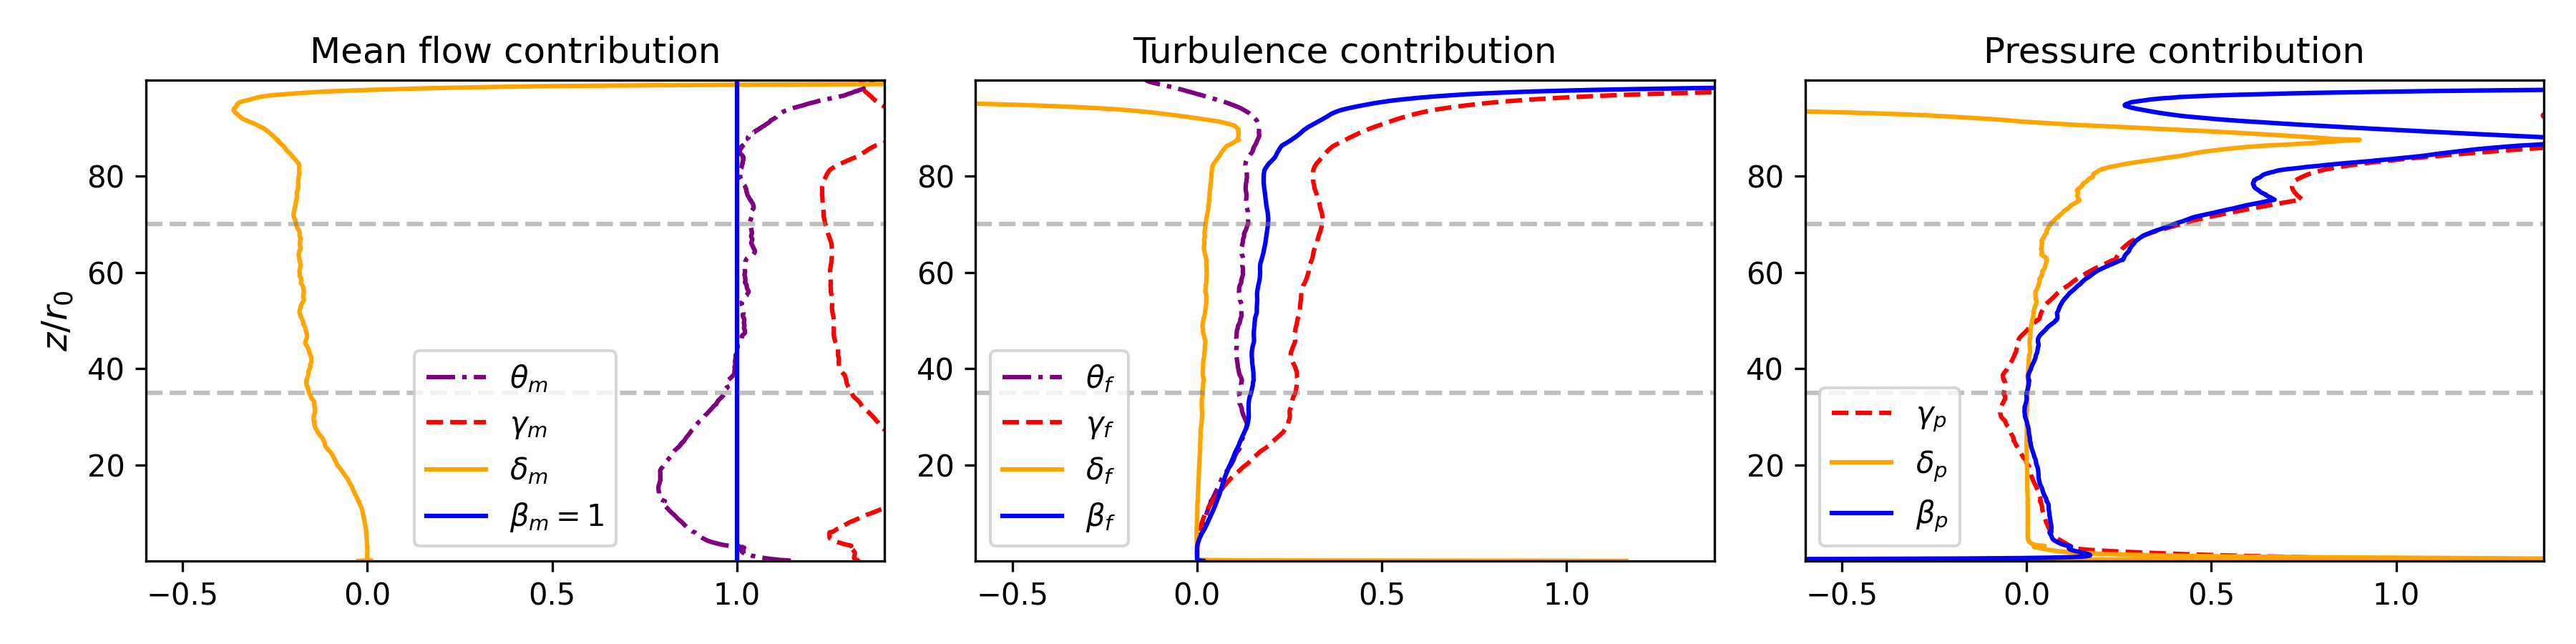
\includegraphics[width=\textwidth]{mvr/fig10}
	\caption{Vertical evolution of mean profile coefficients for mean flow, turbulence and pressure
	contributions.}
	\label{fig:profilecoeff}
\end{figure}

The characteristics of turbulence in the plume may be explored in two ways. Anistropy is investigated by
considering the invariants of the deviatoric component of the Reynolds stress tensor, known as the
anistropy tensor $b_{ij}$ and defined as
\begin{equation}
	b_{ij} = \frac{\overline{u'_iu'_j}}{\overline{u'_iu'_i}} - \frac{1}{3}\delta_{ij}
	\label{eq:anisotropy}
\end{equation}
where $\overline{\cdot}$ is the mean component of an appropriate Reynolds' decomposition. The first invariant
$\mathrm{Tr}(\bm{b})$ is zero and following \citet{lumley1977}, the second and third invariants $\eta, \xi$
are defined as $6\eta^2 = b_{ij}b_{ji} = \mathrm{Tr}(\bm{b}^2)$ and $6\xi^3 = b_{ij}b_{jk}b_{ki} =
\mathrm{Tr}(\bm{b}^2)$. These variables describe any physical state of turbulence in a 2D map known as the
`Lumley triangle'. The second invariant $\eta > 0$ identifies the degree of anistropy in the flow field, where
large $\eta$ indicates strong anisotropy. The third invariant $\xi$ determines if the turbulence state is
one-component, two-component, axisymmetric, etc. In the plume, we expect weak anistropy (small $\eta)$ and
axisymmetric turbulence, indicated by $\xi = \pm \eta$. This is indeed found in the results as shown in
figure~\ref{fig:turbulence} and there is remarkable similarity with the same results presented in VR16.

\begin{figure}
	\centering
	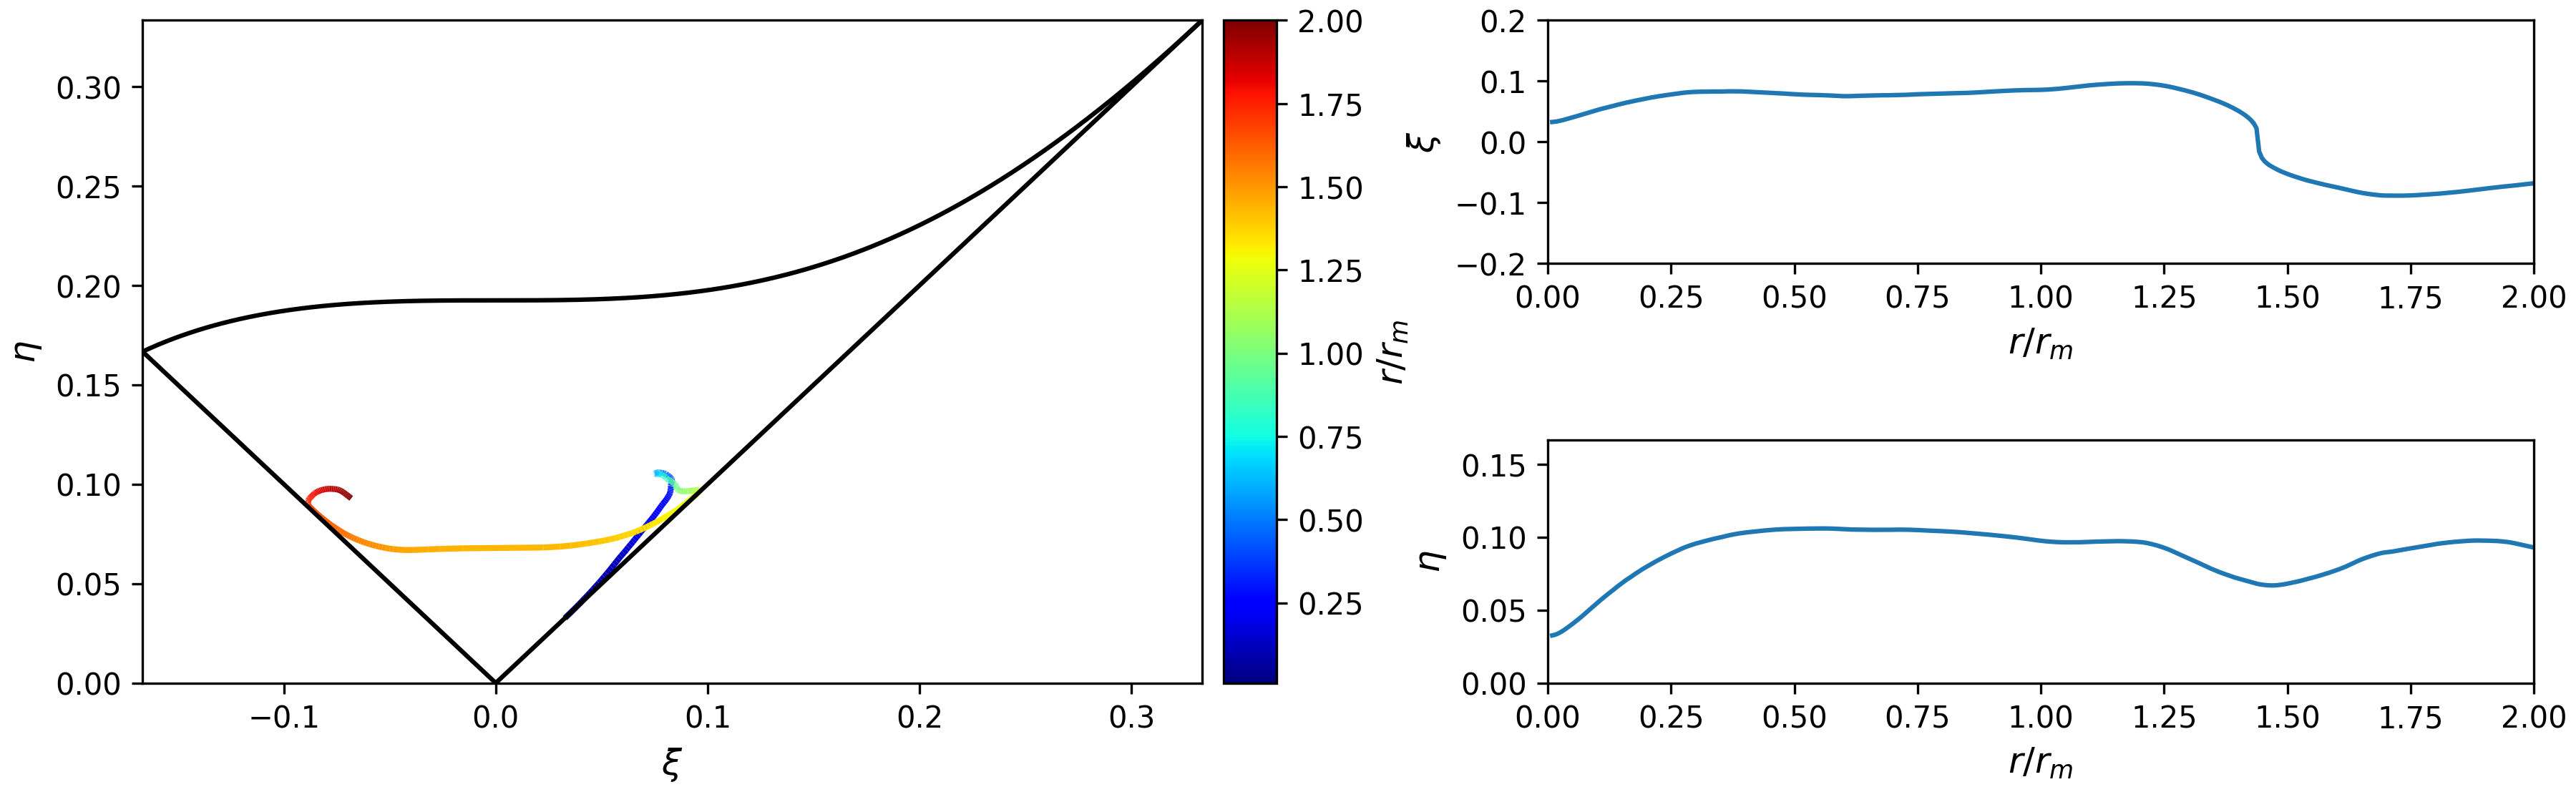
\includegraphics[width=\textwidth]{mvr/fig13}
	\caption{Invariants of the anisotropy tensor \eqref{eq:anisotropy}, plotted in $(\xi,\eta)$ space with the
		Lumley triangle (left), dependence of $\xi, \eta$ on $r/r_m$ (right).}
	\label{fig:turbulence}
\end{figure}

%%%%%%%%%%%%%%%%%%%%%%%%%%%%%%%%%%%%%%%%%%%%%%%%%%%%%%%%%%%%%%%%%%%%%%%%%%%%%%%%%%%%%%%%%%%%%%%%%%%%%%%%%%%%%

\section{Convective penetration into a stably stratified layer}
With the capability for DIABLO to reliably simulate plumes verified and the essential behaviour of a buoyant
plume established, we move closer to the atmospheric case by introducing a stably stratified layer and a
passive tracer carried by the plume. We will explore the dynamics in this stratified case which exhibits the
formation of a `fountain' and a radially spreading intrusion, and compare to similar laboratory experiments in
the literature.

\subsection{Simulation configuration and results}
\label{sec:dynamics}
Figure~\ref{fig:setup} shows a schematic of the simulation setup with an unstratified region of depth $H$ at
the bottom of the domain and a stably stratified region in the remainder of the domain with constant buoyancy
frequency $N^2$. We use the same plume generation method as in the fully unstratified domain, with a source
radius $r_0$ and source buoyancy flux $F_0$. A sponge layer is added in the top $20\%$ of the domain, where
the velocity is damped to remove the reflection of internal gravity waves from the top boundary.  For the
purposes of verifying initial simulation results, the parameters $r_0, H, N^2$ and $F_0$ are computed from the
experimental setup used in laboratory experiments by \citet{ansong2010}. Note that throughout this essay, we
will use physical scales to describe the simulations corresponding to the laboratory context, e.g.\ the
vertical co-ordinate $z$ often uses centimetres. However, rescaling of these quantities is possible, to make
the results relevant to the atmospheric context.

\begin{figure}
	\centering
	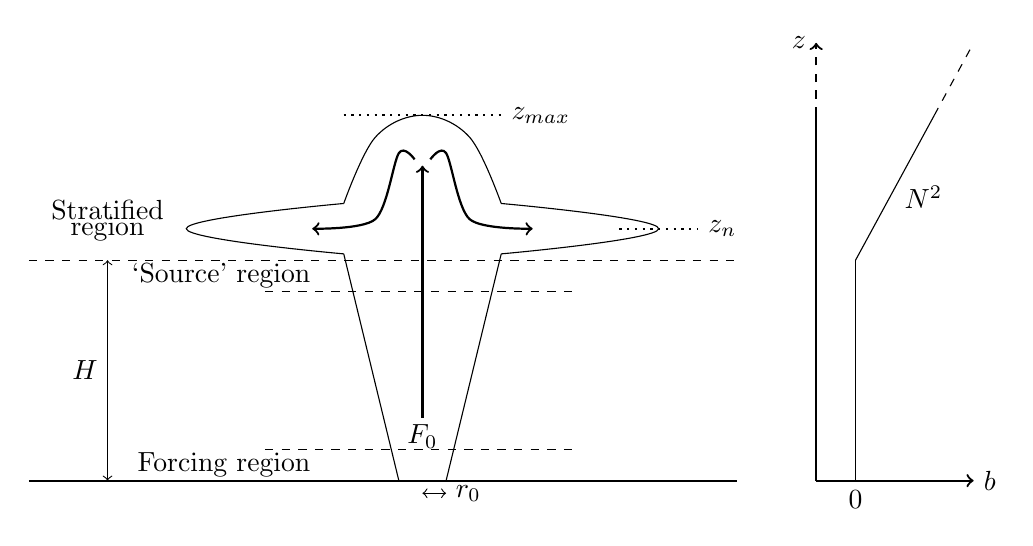
\begin{tikzpicture}[yscale=.8]
		% axes
		\draw[thick] (-5, 0) -- (4, 0);
		\draw[dashed] (-5, 3.5) -- (4, 3.5);

		\draw[<->] (-4, 0) -- (-4, 3.5) node[midway, left] {$H$};
		\draw[<->] (0, -0.2) -- (0.3, -0.2) node[right] {$r_0$};

		\draw[dashed] (-2, 0.5) -- (2, 0.5);
		\draw[dashed] (-2, 3) -- (2, 3);
		\draw (-1.3, 3.25) node[left] {`Source' region};
		\draw (-1.3, 0.25) node[left] {Forcing region};
		\draw (-4, 4.3) node {Stratified};
		\draw (-4, 4) node {region};
		\draw (0, 0.7) node {$F_0$};

		\draw[thick, dotted] (2.5, 4) -- (3.5, 4) node[right] {$z_n$};
		\draw[thick, dotted] (-1, 5.8) -- (1, 5.8) node[right] {$z_{max}$};

		\draw[thick, ->] (0, 1) -- (0, 5);
		\draw[thick, smooth, ->] plot coordinates {(0.1, 5.1) (0.3, 5.2) (0.6, 4.15) (1.4, 4)};
		\draw[thick, smooth, ->] plot coordinates {(-0.1, 5.1) (-0.3, 5.2) (-0.6, 4.15) (-1.4, 4)};

		\draw[smooth, tension=0.6] plot coordinates {(-1, 4.4) (-0.6, 5.45) (0, 5.8) (0.6, 5.45) (1, 4.4)};
		\draw[smooth, tension=0.8] plot coordinates {(1, 4.4) (3, 4) (1, 3.6)};
		\draw[smooth, tension=0.8] plot coordinates {(-1, 4.4) (-3, 4) (-1, 3.6)};
		\draw (1, 3.6) -- (0.3, 0);
		\draw (-1, 3.6) -- (-0.3, 0);

		\draw[thick, ->] (5, 0) -- (7, 0) node[right] {$b$};
		\draw[thick] (5, 0) -- (5, 5.8);
		\draw[thick, dashed, ->] (5, 5.8) -- (5, 6.95) node[left] {$z$};
		\draw (5.5, 0) -- (5.5, 3.5);
		\draw (5.5, 3.5) -- (6.5, 5.8);
		\draw[dashed] (6.5, 5.8) -- (7, 6.95);
		\draw (5.5, 0) node[below] {$0$};
		\draw (6, 4.5) node[right] {$N^2$};

	\end{tikzpicture}
	\caption{Simulation setup and key quantities \& regions for convective penetration of a buoyant plume into
	a stratified layer.}
	\label{fig:setup}
\end{figure}

To aid in the examination of the flow evolution and mixing, we include a passive tracer $\phi$ satisfying the
same dynamical equation as buoyancy. The tracer -- an arbitrary scalar -- is passive in the sense that it has no
coupling with the momentum equation so does not influence the dynamics, it simply follows the flow. The
field $\phi$ represents the tracer concentration, which diffusives according to an associated diffusivity
$\kappa_\phi$ which for convenience is the same as the diffusivity of buoyancy here but may differ in general,
as well as an eddy diffusivity $\kappa_{\phi, T}$. The turbulent diffusivity is computed by the LES model and
accounts for sub-grid scale diffusion. This may locally exceed the prescribed diffusivity by several orders of
magnitude. The tracer is forced using the same volumetric method as the buoyancy, giving a constant source of
tracer with a Gaussian radial profile in the forcing region. Note that regardless of the forcing profile,
turbulent mixing in the plume results in the azimuthally averaged tracer concentration having a Gaussian
profile far from the source.

\begin{figure}
	\centering
	\makebox[\textwidth][c]{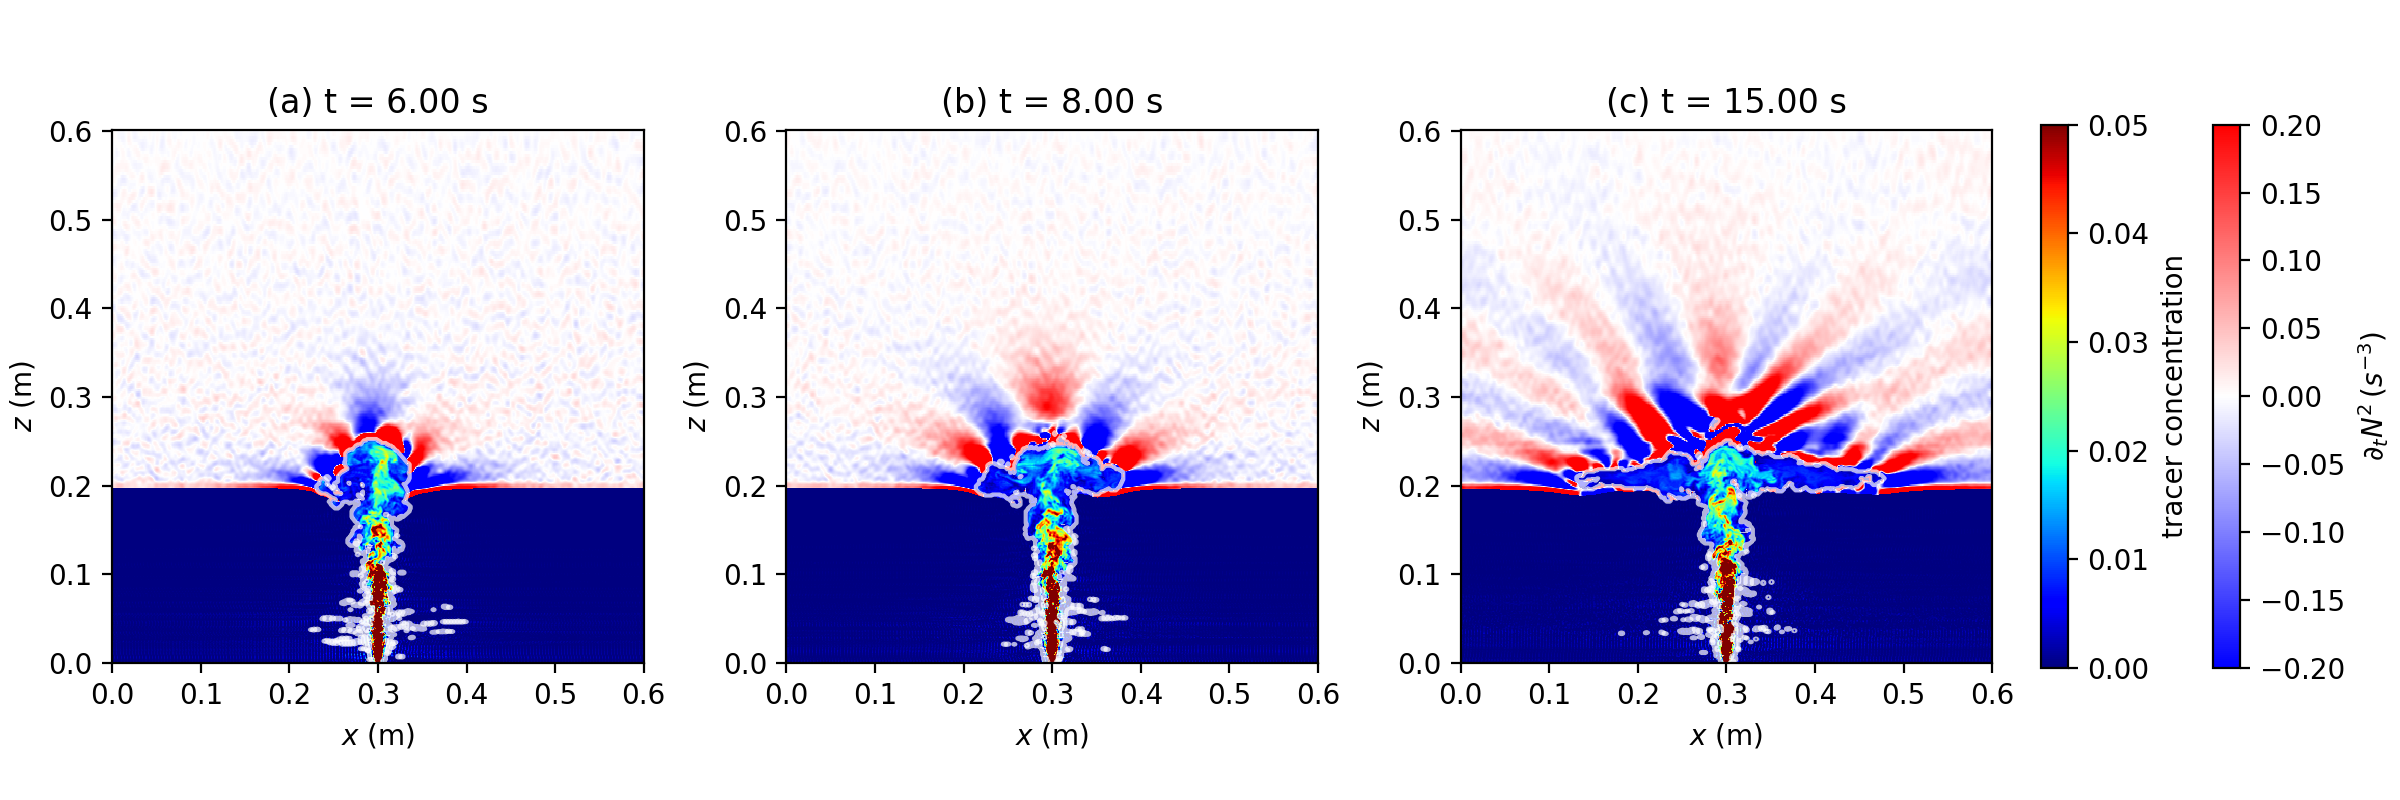
\includegraphics[width=1.15\textwidth]{evolution}}
	\caption{Stages of buoyant plume penetration into a stratified layer at $z=0.2\, \mathrm{m}$. Passive
	tracer field shown inside white contour, wave field representation $\partial_t N^2$ shown outside
	white contour. Note that Gibbs ringing artefacts are visible in the lower part of the domain. Simulation
	with $H = 20\,\mathrm{cm}, r_0 = 0.2 \, \mathrm{cm}, F_0 = 0.15r_0^2 \, \mathrm{m}^4 \mathrm{s}^{-3}$ and
	$N = 1.75\, s^{-1}$.}
	\label{fig:evol}
\end{figure}

Figure~\ref{fig:evol} shows the tracer concentration within white contours and the wave field $\partial_t N^2$
outside, representing the flow evolution which proceeds as follows. Initial penetration of the plume cap
results in generation of internal gravity waves over a range of frequencies, and without subsiding fluid the
plume reaches its maximum penetration height (figure~\ref{fig:evol}(a)) around $t \sim 6 s$. At this stage,
internal gravity waves are beginning to propagate away from the plume cap. As the plume pushes into the
stratified layer, the relative buoyancy becomes negative and the plume fluid overturns and subsides. At $t
\sim 8 s$, further internal gravity waves are produced, now in a more regular pattern, with similar amplitude
to the initial waves (figure~\ref{fig:evol}(b)). The subsiding fluid falls to its level of neutral buoyancy
and spreads as an intrusion (figure~\ref{fig:evol}(c)). At $t \sim 15 s$ the waves cover the entire region
above the spreading current and appear to have a narrow frequency band (i.e.\ most waves at the same angle).
Furthermore, the highest amplitude waves can be traced back to the oscillating plume cap, with some additional
waves produced by the spreading intrusion. These results match qualitatively with studies in the literature,
e.g.\ \citet{ansong2010, hunt2015, devenish2010}.

\subsection{Comparison with lab experiments}

\begin{figure}
	\centering
	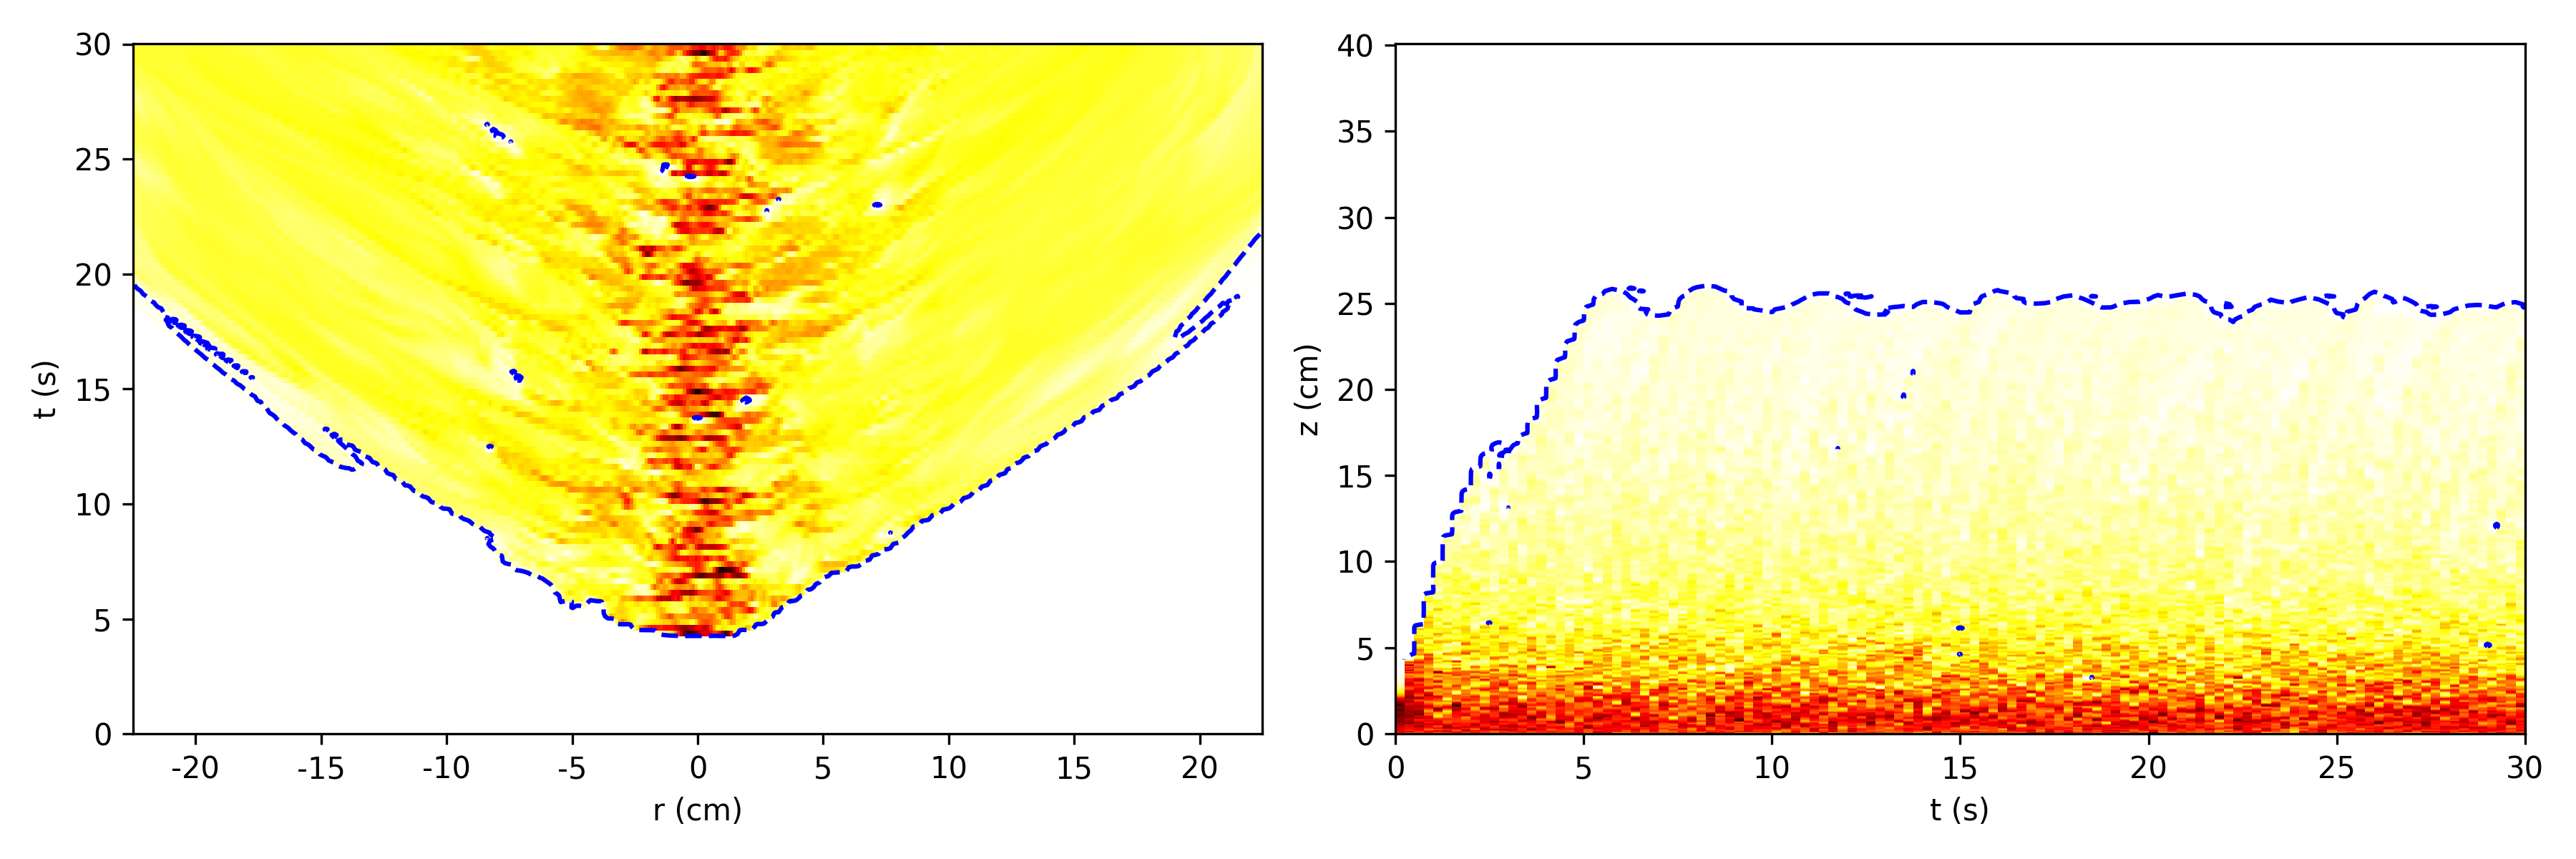
\includegraphics[width=.9\textwidth]{timeseries}
	\caption{Horizontal (left) and vertical (right) time series of the same simulation shown in
		figure~\ref{fig:evol}. The horizontal time series is formed of slices taken at the neutral buoyancy
		level $z \approx 20.9 \, \mathrm{cm}$ and the vertical time series is formed of slices through the
		plume centreline. Colour represents the tracer concentration and the blue dashed line indicates the
		tracer contour used for calculations.}
	\label{fig:timeseries}
\end{figure}

To demonstrate quantitative agreement between our simulations and similar studies in the literature, we
perform analyses of the maximum penetration height $z_{\max}$, neutral buoyancy height $z_n$ and intrusion
spreading rate $V_r$. These quantities are computed by considering horizontal and vertical time series through
the plume centreline; see figure~\ref{fig:timeseries} which emulates the experimental method used by
\citet{ansong2010}, henceforth AS10. The left-hand figure shows horizontal slices of the tracer field taken
at the level of neutral buoyancy (calculation discussed in the next subsection) and through the plume
centreline, showing the intrusion spreading radially. The right-hand figure shows vertical slices of the
tracer field through the plume centreline, showing the plume penetrating into the stratified layer at $H=20 \,
\mathrm{cm}$, reaching its maximum height $z_{\max}$ then oscillating about the quasi-steady-state height
$z_{ss}$. Note that whilst AS10 perform experiments with $H = 0, 5, 10, 15 \, \mathrm{cm}$, as discussed in
appendix~\ref{app:limitations}, we are limited to larger values of $H$ so that the plume may become fully
developed. We consider $H = 10, 15, 20 \,\mathrm{cm}$.

Qualitatively, the results matches those of AS10, with the maximum penetration height remaining well above the
bottom of the stratified layer and the neutral buoyancy height slightly above, as expected from the simulation
parameters. In particular, figure~\ref{fig:zcomp}(a) and (b) show that for $H = 10, 15, 20 \,\mathrm{cm}$ we find a similar
range of maximum penetration heights and neutral buoyancy heights. Note that we find fewer values of $z_n <
0.5 \,\mathrm{cm}$ in our simulations; this discrepancy could be attributed to the fact we can precisely
generate a linear stratification profile with fixed $N^2$ in the simulations, but this is not necessarily the
case in the lab. The generally worse predictions for the $H = 10 \, \mathrm{cm}$ case suggest the unstratified
layer is not deep enough for the plume to become fully developed. There are two other differences present when
comparing our data with AS10.  Figure~\ref{fig:zcomp} (c) shows the ratio of the quasi-steady-state height
$z_{ss}$ and $z_{\max}$ versus the interfacial Froude number
\begin{equation}
	\mathrm{Fr}_i = \frac{\overline{w}_i}{\left( \overline{b}_i \overline{r}_i\right)^{1/2}}
\end{equation}
where the overbar represents a temporal average over the entire simulation post-penetration, as well as a
spatial average over the width of the plume, and subscript $i$ represents the value at the interface. In our
simulations, we find a much smaller range of $z_{ss}/z_{\max}$ compared to that in AS10, though we also sample
a smaller range of interfacial Froude numbers. However, in agreement with AS10, no particular correlation
between $\mathrm{Fr}_i$ and $z_{ss}/z_{\max}$ is found. Similarly, no correlation is found between $H$ and
$\mathrm{Fr}_i$, as one may expect, since for an unstratified plume in the lower region $w_i \sim H^{-1/3}, \,
b_i \sim H^{-5/3}, \, r_i \sim H$ according to the MTT analytic solution of
\eqref{eq:plume1}--\eqref{eq:plume3}, hence $\mathrm{Fr}_i \sim 1$. For the case of a fountain in a linearly
stratified environment, \citet{bloomfield1998} found an average $z_{ss}/z_{\max} \approx 0.93$.
Figure~\ref{fig:zcomp} (d) shows the radial intrusion spreading rate $V_r$ in the simulations versus the ratio
of momentum flux to volume flux at the neutral buoyancy height $M_n/Q_n$. AS10 find a relationship of the form
\begin{equation}
	V_r = (0.12 \pm 0.02) \frac{M_n}{Q_n}
\end{equation}
which is plotted as a dashed grey line in the figure. Evidently our simulation results do not match this
relationship, though a small range of $M_n/Q_n$ is sampled. Nonetheless, we find the range of spreading rates
$V_r$ broadly matches the range found in AS10, and we find a similar range of $M_n/Q_n$ compared with AS10 for
the sampled values of $H$. Together, these results demonstrate that our simulations of a plume penetrating a
stably stratified layer are reliably capturing the dynamics seen in laboratory experiments of the same setup.

\begin{figure}
	\centering
	\makebox[\textwidth][c]{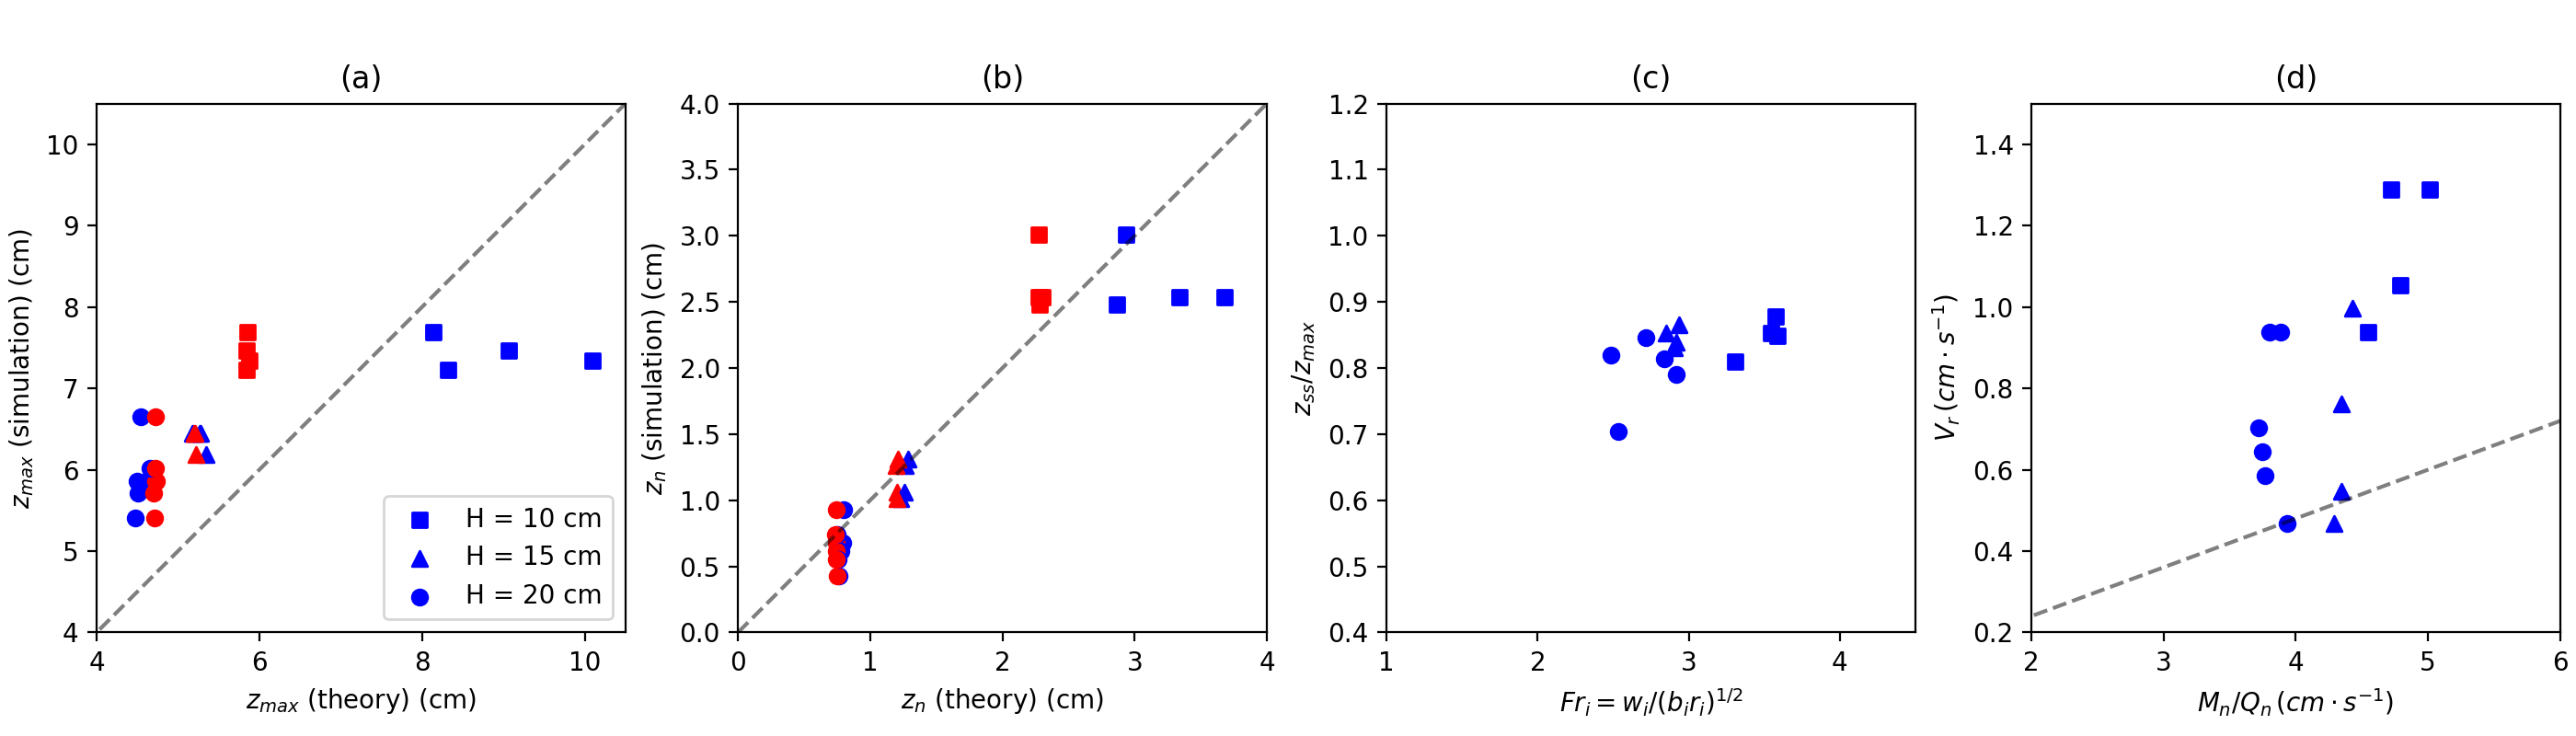
\includegraphics[width=1.1\textwidth]{zcomp}}
	\caption{Comparisons of (a) maximum penetration height and (b) neutral buoyancy height between simulation
	and theory; (c) quasi-steady-state height versus interfacial Froude number; (d) radial intrusion spreading
	rate versus ratio of momentum and volume fluxes. In (a) and (b), the AS10 numerical method is shown in
	blue, and the simplistic approximation detailed in section~\ref{sec:zmax} is shown in red.} 
	\label{fig:zcomp}
\end{figure}

\subsection{Estimates of maximum penetration height}
\label{sec:zmax}
The maximum penetration height is of central importance in this problem, as it determines the maximum level
of fluid detrainment \citep{ansong2008} and in the atmospheric case, it is directly linked to temperature
constraints on the concentration of water vapour \citep{jensen2007}. The TTL contains the `cold-point
tropopause' defined as the minimum of the temperature profile \citep{fueglistaler2009}; if the maximum
penetration height of a convective overshoot exceeds this altitude and reaches larger temperatures, then the water
vapour transported to this altitude is more likely to remain in the stratosphere as greater potential
temperatures are accessed. Furthermore, as the environmental temperature increases, the sublimation of ice
hydrometeors is aided. This process is critical to determining whether a convective overshoot ultimately
hydrates the stratosphere \citep{dauhut2018}.

AS10 compute predictions of $z_{\max}$ and $z_n$ using a numerical method whereby the MTT plume equations are
numerically solved using values of $M, F$ and $Q$ evaluated at the interface $z=H$ as initial conditions. In
this method, $z_{\max}$ is defined as the point where the momentum flux $M$ vanishes, and the neutral buoyancy
height is where the buoyancy flux $F$ vanishes. Application of the same method to our simulation data is shown
in figures~\ref{fig:zcomp}(a) and (b). The grey vertical lines indicate the interfacial values of $M, F$ and
$Q$ used as initial conditions. The neutral buoyancy height is well predicted, as was found in AS10. The
maximum penetration height is generally underpredicted by this method, with values on average $80\%$ of the
true value. Examining the numerical solutions for $M, F$ and $Q$ compared to the actual fluxes in
figure~\ref{fig:fluxes} shows that the reasonable agreement found is perhaps surprising, as the numerically
solved flux profiles do not resemble the simulated fluxes. $M$ is perhaps the closest representation, but $F$
and $Q$ do not represent the data well and as the three variables are coupled, the efficacy of this technique
could be questioned. This itself is not unsurprising: the MTT equations as applied assume there is no mixing
of ambient fluid between the neutral level and the maximum height, which would raise the maximum height if
accounted for, as plume fluid entrains positively buoyant fluid. In any case, the MTT assumption that
entrainment is proportional to axial velocity breaks down once the plume becomes a fountain in the stratified
region, so equations \eqref{eq:plume1}--\eqref{eq:plume3} should not be applicable. Note that
figure~\ref{fig:fluxes} shows the \emph{full} fluxes, calculated over the entire domain, and the
\emph{thresholded} fluxes, representative of the flux inside the plume (or the rising component of the
fountain) itself. Whilst one might expect the thresholded flux within the plume would yield the best estimate,
this is the case for $z_n$ but using the full fluxes as initial conditions produces the best estimates for
$z_{\max}$ as demonstrated in the figure. Further corrections may be applied to the MTT equations to refine
this technique, for example the `unaltered volume flux' method, which numerically solves $F$ and $M$ using the
unstratified $Q$-profile. \citet{devenish2010} use this technique to argue that the reasonable agreement found
with $z_n$ suggests that stratification does not play a significant role below the neutral buoyancy height.

\begin{figure}
	\centering
	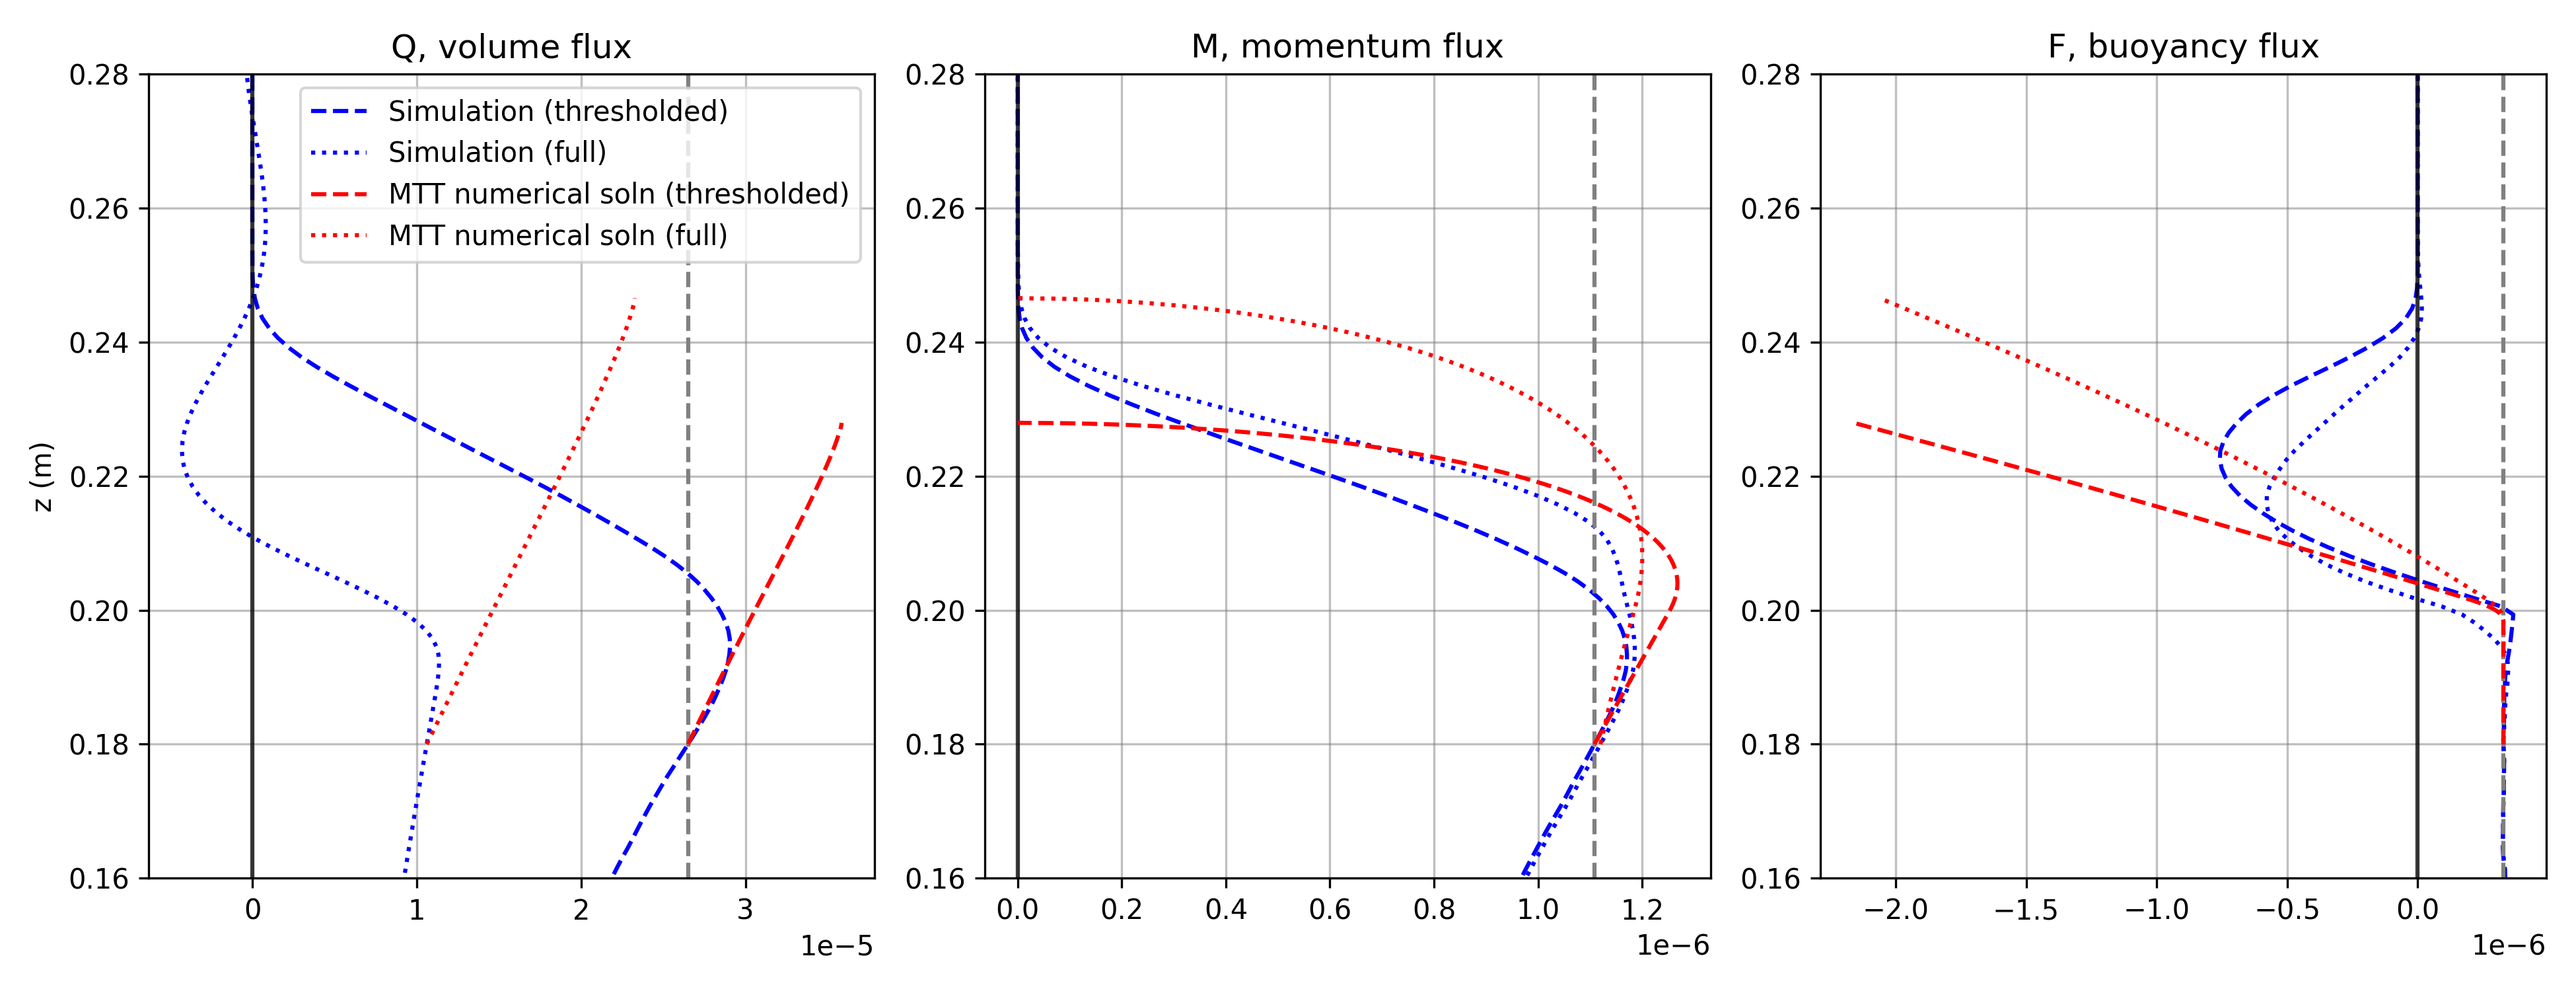
\includegraphics[width=\textwidth]{fluxes}
	\caption{Vertical profiles of volume, momentum and buoyancy flux within the plume (thresholded) and across
		the entire domain (full). Blue lines indicate the profiles computed from simulations in DIABLO, red
		lines indicate profiles from numerically solving the MTT plume equations
		\eqref{eq:plume1}--\eqref{eq:plume3} with initial conditions taken from simulation results at the
		bottom of the stratified layer. Data from the same simulation as figure~\ref{fig:evol}.}
	\label{fig:fluxes}
\end{figure}

More simplistic methods may be used to estimate $z_{\max}$ and $z_n$. In some cases,
non-dimensionalised numerical solutions of the MTT equations can be fitted to LES data, e.g.\
\citet{devenish2010}. The maximum penetration height may also be estimated via a simplistic energetic
argument: the kinetic energy density at penetration, $E_k(H)$, and potential energy density at height $z$,
$E_p(z)$, on the centreline are
\begin{align}
	E_k(H) &= \frac{1}{2}\rho (2 w_m)^2 = \frac{1}{2}\rho \left[4 \cdot \left(\frac{5}{6\alpha}\right)^2
		\left(\frac{9}{10} \frac{\alpha}{\theta_m \beta_g} F_0\right)^{2/3} H^{-2/3}\right]\\
	E_p(z) &= \frac{1}{2}\rho N^2 (z-H)^2
\end{align}
Neglecting dissipation and assuming that all KE is converted to PE at $z=z_{\max}$, we find
\begin{equation}
	z_{\max} = \frac{2}{N} \left(\frac{5}{6\alpha}\right)\left(\frac{9}{10}\frac{\alpha F_0}{\theta_m \beta_g}
		\right)^{1/3} \left(H-z_v\right)^{-1/3} \sim \alpha^{-2/3} F_0^{1/3} H^{-1/3} N^{-1} 
\end{equation}
A similarly simplistic argument for the neutral buoyancy height assumes that without mixing, fluid will come to
rest at the level with the same environmental buoyancy as the average plume buoyancy at penetration
$\overline{b}_i$ = 2$b_m(H)$. Hence, the neutral buoyancy height is approximately
\begin{equation}
	z_n = \frac{5F_0}{3\alpha \theta_m N^2} \left(\frac{9}{10}\frac{\alpha}{\beta_g \theta_m}
	F_0\right)^{-1/3} \left(H-z_v\right)^{-5/3} \sim \alpha^{-4/3} F_0^{2/3} H^{-5/3} N^{-2}
\end{equation}
Figure~\ref{fig:zcomp} shows these estimates for each simulation in red, compared with the AS10 method in
blue. The same relationships are seen; $z_{\max}$ is underpredicted whilst $z_n$ is reasonably well predicted,
illustrating in this case that simplistic methods sometimes exhibit the same predictive value as more complex
methods.

In the atmospheric case, there are many complications which play a role in setting the penetration depth
of a convective plume. For example, latent heating in the rising plume effectively increases the buoyancy
flux at penetration. This can be accounted for in simulations (which neglect latent heat) by increasing the
source buoyancy flux. As a further example of the complexity, \citet{tailleux2004} discuss the need for a
correction to the concept of Convective Available Potential Energy (CAPE), computed from the work done by a
fluid parcel relative to an environmental sounding up to the level of neutral buoyancy, assuming undiluted
ascent. This overestimates the energy available for converting to KE, and therefore the penetration depth, for
two reasons: the mass of the condensed water retained during adiabatic ascent, and the negative work due to
subsidence of the central updraft. Even in the idealised fluid problem considered thus far, the ideas behind
these concepts could be incorporated, for example by subtracting the work done against the subsiding component
of the fountain from the KE available for converting to PE, yielding a prediction for the quasi-steady-state
height.

Whilst important, estimating the maximum penetration height does not solely answer the questions posed for
this problem; $z_{\max}$ determines the maximum \emph{accessible} environmental buoyancy, but the level at
which mixing occurs, and the buoyancy of the plume fluid which most efficiently mixes with the environment,
determines the final buoyancy of the mixed fluid and therefore whether tracer remains in the stratified layer.
Nonetheless, the value of the environmental buoyancy at height $z_{\max}$ offers a useful constraint on the
buoyancy of mixed fluid as will be demonstrated in section~\ref{sec:jointPDF}.

\subsection{Internal gravity waves}

The generation of internal gravity waves, visualised in figure~\ref{fig:evol}, is an interesting
component of this problem for many reasons, though we will only mention it briefly here. Whilst the wave
energy flux is a relatively small proportion of the input energy flux by the plume, in the atmospheric case,
the dominant wave modes have been shown to modify the immediate cloud environment \citep{lane2001}, which may
facilitate the saturation of stratospheric air surrounding the convective overshoot. Furthermore, gravity
waves generated by deep convection play a role in many atmospheric processes; for example, high frequency
gravity waves are thought to make a significant contribution to the momentum flux which drives the QBO
\citep{baldwin2001}. \citet{flynn2004} found the total vertical momentum flux from gravity waves forced by
overshooting convection is comparable to topographically forced waves, and since convectively generated
waves arise in the UTLS and have non-zero phase speeds, they can propagate upwards and contribute to the
gravity wave spectrum driving the QBO. There also remains debate over the dominant wave generation mechanism
and the frequency spectrum of the generated waves. 

The introduction of shear would allow comparison of the contributions of some of the 
wave generation mechanisms hypothesised for deep convection. The three leading contenders for this 
mechanism are: the perturbation of the mean flow caused by the pressure field above a rising convective cell,
known as the `obstacle effect'; the oscillatory deflection of the boundary of the stratified layer, known as
the `mechanical oscillator'; and the `deep heating effect' as a result of latent heat release
\citep{flynn2004}. Without a mean flow or latent heating, future work will focus on the mechanical oscillator.
We may then establish the energy and momentum flux associated with waves generated by this mechanism, and
compare the results with simulations including large-scale shear to compare the contribution from each of the
`obstacle effect' and 'mechanical oscillator' mechanisms.

%%%%%%%%%%%%%%%%%%%%%%%%%%%%%%%%%%%%%%%%%%%%%%%%%%%%%%%%%%%%%%%%%%%%%%%%%%%%%%%%%%%%%%%%%%%%%%%%%%%%%%%%%%%%%

\section{Tracer transport}
\label{sec:tracertransport}
Having explored the idealised setup with which we study the atmospheric problem, including understanding the
role of key parameters such as $z_{\max}$ and $z_n$, we move on to considering the passive tracer carried by
the plume. 

\subsection{Tracer distributions in buoyancy coordinates}
\label{sec:distributions}

Mixing is an irreversible process in which the properties of distinct fluid parcels are combined and modified.
The blending of properties of fluid elements which mix is driven by molecular diffusion, which itself
is promoted by turbulence. In a stratified flow, the critical property to understand is the buoyancy of a
fluid element as this will determine its position once any transient dynamics have subsided and the fluid
settles. The \emph{irreversible} transport of water vapour and other tracers into the stratosphere thus
requires fluid parcels carrying tracer to change buoyancy. Therefore, it is of interest to examine the
distribution of passive tracer in buoyancy space, where mixing will act to move tracer concentrations to
different buoyancies, indicating the diapycnal transport of tracer taking place. 

The turbulent mixing of fluid parcels can be considered a two-step process \citep{wykes2014}, composed of
stirring and diffusion. Stirring geometrically deforms fluid parcels and stretches surfaces of
constant buoyancy, increasing the area over which molecular diffusion acts. Moreover, stirring strengthens
buoyancy gradients across buoyancy surfaces, further promoting diffusion. Crucially, stirring is -- in
principle -- a reversible process, whilst molecular diffusion is irreversible and we are most interested in
the \emph{irreversible} transport of tracer to greater buoyancies.  Therefore, a benefit of analysing tracer
distributions in buoyancy space is the separation of the effects of stirring and diffusion. Since stirring
only deforms fluid parcels, it does not change the tracer concentration or buoyancy within fluid parcels and
therefore only the diffusive component of mixing results in changes in the tracer distribution in buoyancy
space. 
\begin{figure}
	\centering
	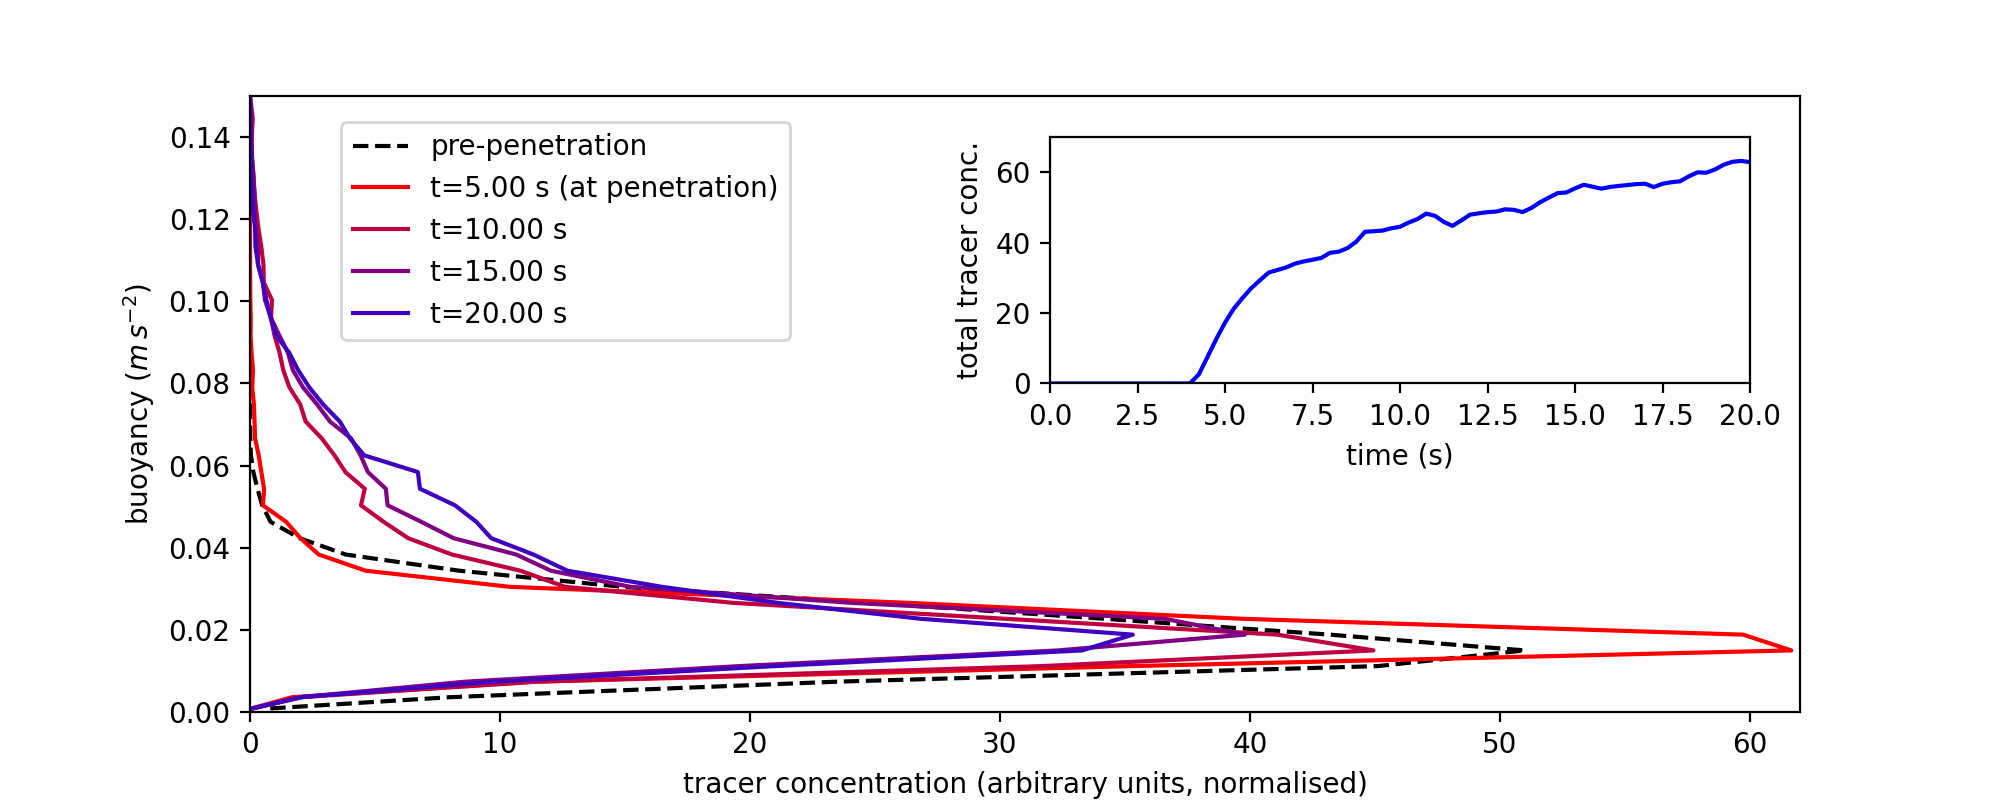
\includegraphics[width=.6\textwidth]{tb_dist}
	\caption{Normalised tracer distribution in buoyancy coordinates in the stratified region indicated in
		figure~\ref{fig:setup}. Coloured lines are distributions post-penetration at equal time intervals,
		black dashed line is the time-averaged pre-penetration distribution from the `source region' indicated
		in figure~\ref{fig:setup}. Evolution of total tracer concentration (arbitrary units) in the stratified
		layer inset. Composite of 5 identical simulations (with random perturbations) with $H =
		20\,\mathrm{cm}, r_0 = 0.2 \, \mathrm{cm}, F_0 = 0.15r_0^2 \, \mathrm{m}^4 \mathrm{s}^{-3}$ and $N =
		1.75 s^{-1}$.}
	\label{fig:tbdist}
\end{figure}

Figure~\ref{fig:tbdist} shows a composite over several simulations of the tracer distribution in buoyancy
coordinates in the stratified region at multiple times.  These distributions are normalised to have unit area,
and therefore referred to as a PDF henceforth. Note that the total tracer concentration in the stratified
region increases with time (see figure~\ref{fig:tbdist} inset), so the unnormalised area under the curve
increases with time. The normalisation therefore allows comparison of tracer distributions at both early and
late times.  A composite is taken to compensate for the random perturbations applied to the forcing profile. A
`source' PDF is taken from a thin layer immediately beneath the stratified layer, referred to as the source
region (see schematic in figure~\ref{fig:setup}), which represents the tracer distribution in the plume
\emph{before} penetrating the stratified region.  Mixing as a result of the penetration process manifests as
changes in the PDF. In particular, the mixing of plume fluid containing tracer with more buoyant environmental
fluid in the stratified region has two effects, seen as two differences between the black and coloured lines.
Fluid parcels with low buoyancies, i.e.\ those carrying small amounts of tracer at large radii within the
plume, immediately encounter more buoyant fluid and mix, giving rise to the decrease in tracer between the
source and post-penetration distributions at low buoyancy. Plume fluid that penetrates deep into the
stratified region and mixes with much more buoyant environmental fluid produces the increasing `mass' of the
tracer distribution tail at large buoyancies.

\begin{figure}
	\centering
	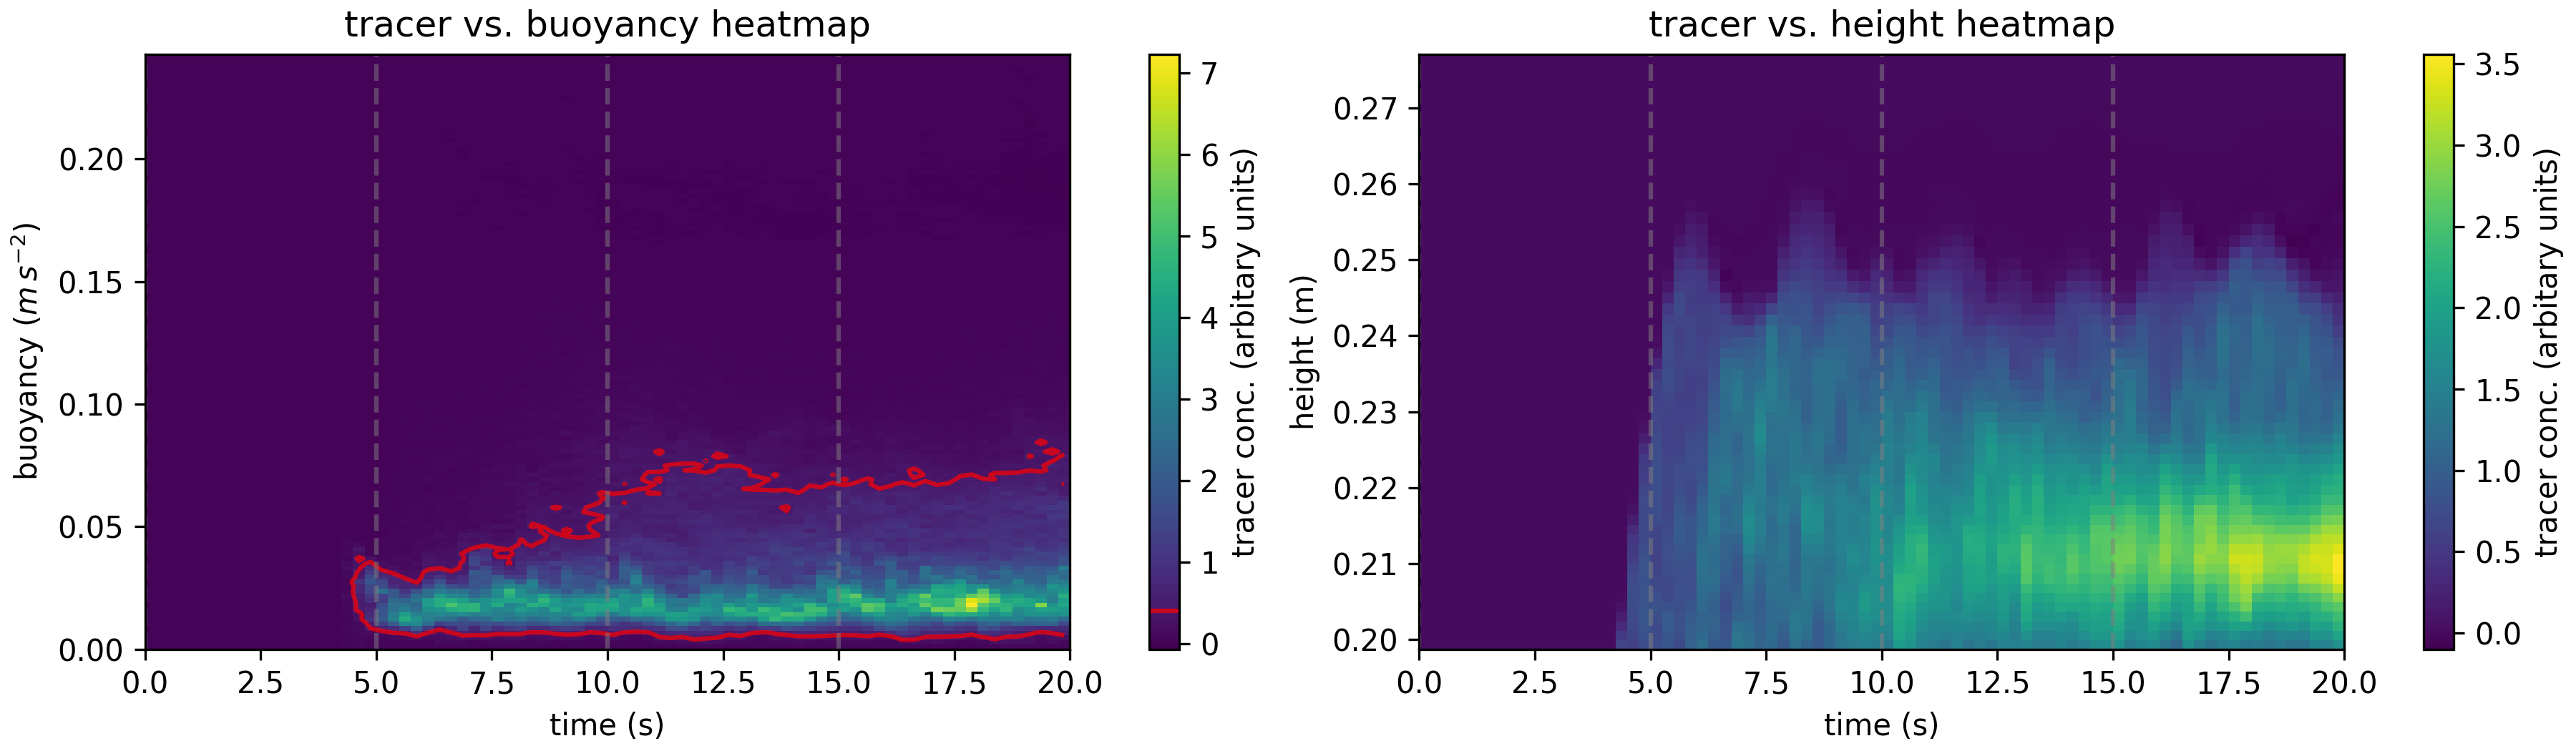
\includegraphics[width=\textwidth]{hmap}
	\caption{Distribution as described in figure~\ref{fig:tbdist}, but shown in buoyancy (left) and height
		(right) coordinates evolving over time. No normalisation is applied to the distributions. Data from
		simulations with the same parameters as in figure~\ref{fig:tbdist}.} 
	\label{fig:hmap}
\end{figure}

Whilst figure~\ref{fig:tbdist} is useful for comparing the distribution shape at different times, the
dynamical changes and the change in distribution peak are better visualised in a heatmap as shown in
figure~\ref{fig:hmap}.  Moreover, we can also compare the tracer distribution in buoyancy and height
coordinates. The horizontal axis shows evolution in time, with colour representing the amount of tracer; in
this case, unnormalised, so that the increase in tracer with time is apparent. Nonetheless, we will continue
to refer to the distributions as a PDF for convenience. The vertical axes are scaled so that the scales of
buoyancy and height coincide, i.e.\ for the background buoyancy profile, the buoyancy in the left panel
corresponds to the height in the right panel. This is verified by noting that at late times, the majority of
tracer settles at its neutral buoyancy height, and this level with concentrated tracer in the height and
buoyancy heatmaps coincides. Note that the ambient stratification $N^2$ defines the background buoyancy
profile used to link buoyancy and height, but the ambient buoyancy gradient surrounding the plume tends to be
weakened by the penetrating plume (note the widening buoyancy contours at the bottom of the stratified layer
in the top panels of figure~\ref{fig:mixingregions}), so tracer can reach much larger heights than the
corresponding environmental value of buoyancy. The tracer vs.\ height view shows the oscillation of the plume
around its quasi-steady-state height as well as the collection of tracer in the intrusion. The tracer vs.\
buoyancy view demonstrates that the distribution at late times is largely similar to that immediately
post-penetration at small buoyancies, but there is a significant fraction of tracer that reaches larger
buoyancies. However, whilst tracer has reached its maximum height at $t \approx 6 \, s$, the presence of
tracer at larger buoyancies only becomes evident around $t \approx 10\,s$, indicating that the mixing
timescale is perhaps longer (slower) than the dynamical timescale -- note the red contour on the left panel at
a low tracer threshold, which only reaches buoyancies greater than $\sim 0.05$ around $t \approx 10\,s$. It
also appears that the most `effective' mixing events, those where there is a notable increase in tracer at
larger buoyancies, coincide with larger amounts of tracer being lifted to heights approaching $z_{\max}$,
which is likely as a result of the largest eddies (carrying the most tracer) reaching their maximum height.

\subsection{Buoyancy-tracer volume distributions}

A limitation of the tracer PDF considered thus far is the lack of information on the distribution of tracer at
a given buoyancy value; whilst at some buoyancy there may be a peak in the tracer PDF, this may be due to
relatively few fluid parcels carrying large tracer concentrations or from relatively many fluid parcels
carrying small amounts of tracer; the former results in more effective transport of tracer via mixing.
\citet{penney2020} study mixing by Kelvin-Helmholtz instabilities and use a density-tracer joint PDF to
identify irreversible diffusive mixing. For convenience we instead use a buoyancy-tracer volume distribution,
i.e.\ an unnormalised joint PDF. Here, instead of using the (normalised) total tracer concentration of fluid
parcels with a given buoyancy as a weight in buoyancy coordinates, we use the total volume of fluid with a
given range of buoyancy and tracer as the weight in 2D $(b, \phi)$ coordinates.

\subsubsection{Definition}
Formally, we consider a discrete formulation of the probability function following \citet{plumb2007}, with
weights $W_{ij}(t)$ evolving in time and the normalisation omitted. We consider the stratified layer as the
physical domain, to examine the effects of mixing on tracer and buoyancy in the penetration process rather
than in the rising plume. The buoyancy and tracer domains are subdivided into $N_b$ and $N_\phi$ equally sized
bins of size
\begin{equation}
	\delta b = \frac{b_{\max} - b_{\min}}{N_b}, \hspace{2em} \delta \phi = \frac{\phi_{\max} -
		\phi_{\min}}{N_\phi}
\end{equation}
where we choose $b_{\min} = 0$ and $b_{\max} = N^2 (L_z - H)$ to capture the smallest and largest
environmental buoyancy in the stratified layer, respectively. In cases where the plume does not penetrate a
significant distance into the stratified layer, $b_{\max}$ may be reduced to better resolve the volume
distribution.  Choosing bounds for the tracer domain is more difficult; owing to the turbulent nature of the
plume, it is difficult to place an upper limit on the concentration of tracer. We therefore make a rough
estimate, using the tracer concentration on the plume centreline at penetration height $z=H$ as predicted by
the MTT plume equations:
\begin{equation}
	\phi_{\max}  = k\frac{5F_0}{3\alpha} \left(\frac{9}{10}\alpha F_0\right)^{-1/3} \left(H +
		\frac{5r_0}{6\alpha}\right)^{-5/3}
\end{equation}
where $F_0$ is the source tracer flux, identical to the buoyancy flux. An additional factor $k > 1$ is
included to ensure that random fluctuations of $\phi$ above this azimuthally averaged approximation are still
captured. Tracer concentrations may not be negative so we choose $\phi_{\min} = 0$.

Denoting the centre of a given bin as $(b_i, \phi_j)$, the weight is defined as
\begin{equation}
	W_{ij}(t) = \sum_V I_{ij}(t) \Delta x \Delta y \Delta z
\end{equation}
where $V$ is the volume of the domain under consideration, $\Delta x_i$ are the grid-cell widths, and the
indicator $I_{ij}(t)$ is defined as
\begin{equation}
	I_{ij}(t) = \begin{cases}
		1 & \left(b(\bm{x},t) - b_i, \phi(\bm{x},t) - \phi_j\right) \in \left( -\frac{1}{2}\delta b,
		\frac{1}{2}\delta b \right] \times \left( -\frac{1}{2}\delta \phi, \frac{1}{2}\delta \phi \right] \\
			0 & \text{otherwise}
		\end{cases}
		\label{eq:indicator}
\end{equation}

There are a number of differences between the above formulation and that of \citet{penney2020}. First, we do
not normalise the weights $W_{ij}(t)$ by the total volume of the domain $V$, so that we may modify the weights
by subtracting a similarly-defined weight derived from a domain with a different volume, which is explained in
section~\ref{sec:jointPDF} as a method for identifying mixed plume and environmental fluid. Note that the
normalisation is arbitrary in our context, as we are uninterested in regions with no tracer. We could
artifically increase the volume of the domain without modifying the plume, in which case the normalisation
factor would change but the distribution and its interpretation would not. The weights therefore form an
\emph{unnormalised} joint PDF, and may equivalently be considered as the volume of fluid with buoyancy and
tracer concentration close to $b_i$ and $\phi_j$, so we refer to this as a volume distribution. Finally, note
that plume fluid has non-zero buoyancy by definition, so we wish to exclude fluid elements with zero buoyancy
from the weight. Similarly, to isolate mixed plume and environmental fluid and exclude unmixed ambient fluid,
we wish to exclude fluid containing no tracer. Therefore, the intervals used in defining the
indicator~\eqref{eq:indicator} are open/closed in the opposite sense to \citet{penney2020}; they use intervals
of the form $\left[a, b\right)$ whilst we use intervals of the form $\left(a, b\right]$. The smallest buoyancy
and tracer bins are then of the form $\left(0, \delta b\right]$ and $\left(0, \delta \phi\right]$. 

\subsubsection{Properties}
\label{sec:PDFproperties}
Buoyancy and passive tracer concentration evolve according to advection-diffusion equations without sources or
sinks (outside of the forcing region), which provides a constraint on the evolution of the volume distribution
that proves useful when distinguishing pre- and post-mixed fluid. As discussed in \citet{penney2020},
\citet{plumb2007} and references therein, mixing acts to homogenise the buoyancy and tracer of parcels within
a region whose size is determined by the molecular diffusivities $\kappa_b$ and $\kappa_{\phi}$. The
buoyancy-tracer characteristics of the mixed parcel is then an average of the initial parcels, weighted by
their volumes. We therefore have the constraint that after stirring and diffusive mixing, points in
buoyancy-tracer space are contained within the convex hull of the initial distribution of buoyancy and tracer.
The convex hull is the smallest envelope that contains all non-zero points of the distribution. Since our
domain has a buoyancy and tracer input from the plume, in fact at a given time we must consider the convex
hull of the current distribution combined with the volume distribution of the fluid arriving into the
domain at that time.

A number of useful properties arise from the above constraint, provided the diffusivities of tracer and
buoyancy are the same. As the volume distribution continuously evolves, the distribution at the next time step
must lie within the convex hull of the current time step. We therefore expect extreme values of buoyancy and
tracer to shift towards the mean as a result of mixing. In the absence of a bouyancy or tracer flux, the
convex hull must reduce over time and result in a more compact distribution, but this is not the case for
convective penetration as we have a continuous influx of buoyancy and tracer into the domain. Nonetheless, for
a given range of buoyancy, extreme concentrations of tracer are limited by the cumulative convex hull of the
distribution as new plume fluid arrives in the stratified layer, and by mixing with environmental fluid with
no tracer, the extrema are eroded. Finally, note that the the convex hull of a line is also a line.  Hence if
fluid parcels along a line in buoyancy-tracer space mix, they will remain on that line. As a result,
fluid on a line in buoyancy-tracer space which has not mixed with fluid parcels elsewhere in buoyancy-tracer
space, can be distinguished from fluid which \emph{has} mixed, since mixed fluid will no longer be confined to
the line.

\subsubsection{Results}
The volume distribution weights $W_{ij}(t)$ are represented in colour on a 2D plot in figure~\ref{fig:jointPDF}.
Three instantaneous snapshots of the distribution are shown with an illustrative view of the plume tracer
field and environmental buoyancy contours to demonstrate the associated dynamics. Regions of the volume
distribution which are not coloured indicate that no fluid occupies that region of buoyancy-tracer space.

\begin{figure}
	\centering
	\makebox[\textwidth][c]{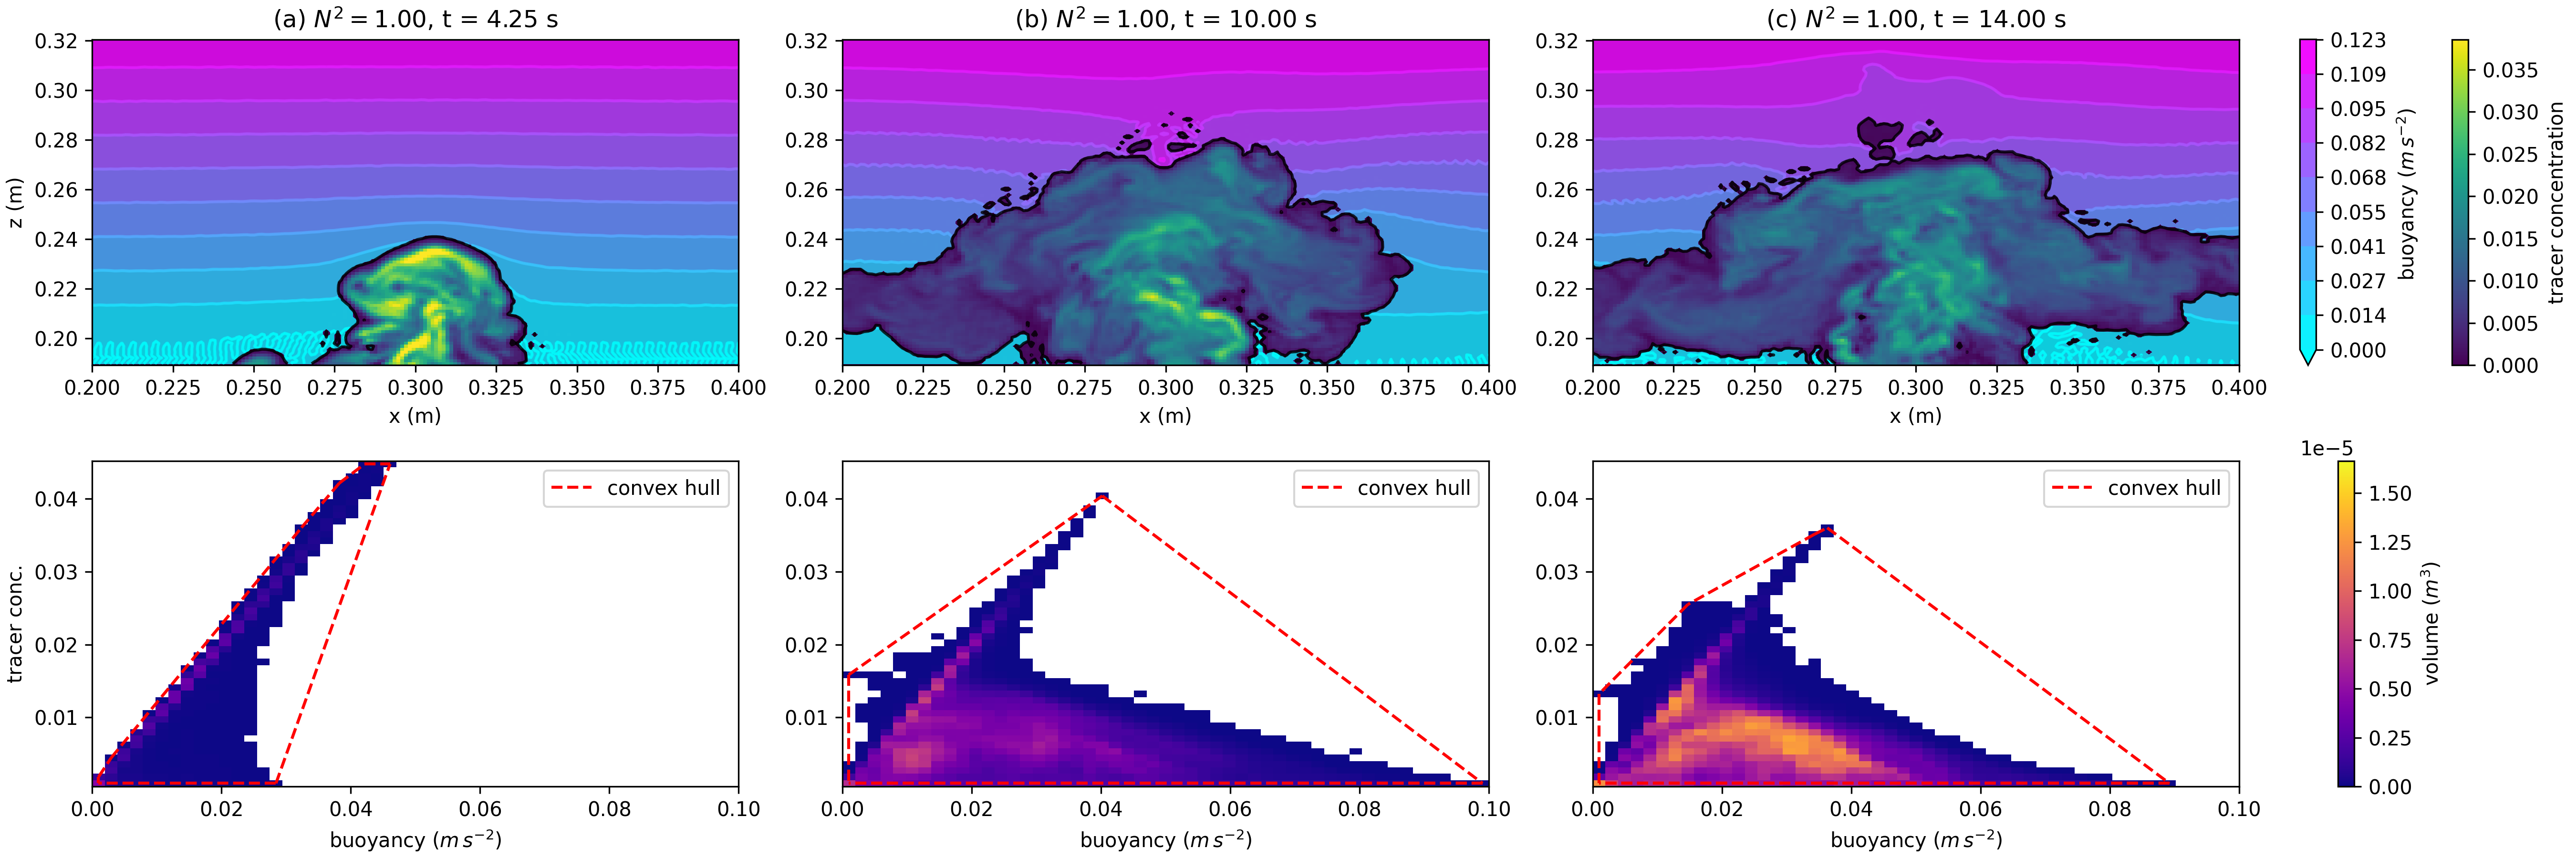
\includegraphics[width=1.2\textwidth]{comp_pdf}}
	\caption{Three instantaneous snapshots of the buoyancy-tracer volume distribution (bottom) with  illustrative view
	of plume tracer field with surrounding environmental buoyancy contours (top). Data from a simulation with
	$H = 20\,\mathrm{cm}, r_0 = 0.2 \, \mathrm{cm}, F_0 = 0.15r_0^2 \, \mathrm{m}^4 \mathrm{s}^{-3}$ and 
	$N = 1.0 \,s^{-1}$.}
	\label{fig:jointPDF}
\end{figure}

Figure~\ref{fig:jointPDF}(a) shows the volume distribution as the plume first penetrates the stratified layer,
with little mixing having taken place. Panel (a) therefore represents the 2D version of the `source'
distribution in figure~\ref{fig:tbdist}, with a wide variation of tracer over a smaller range of buoyancy in
the plume (relative to the stratification). We will discuss the `source' distribution further in the following
subsection. The convex hull shown is that of the distribution at the given time combined with the convex hull
of the volume distribution of plume fluid arriving in the stratified layer up to that time. This
therefore represents the region in which the current buoyancy-tracer distribution must lie at the next time,
though new plume fluid arriving can lie outside this convex hull. Note the small volumes lying outside the
previous convex hull in figures~\ref{fig:jointPDF}(b) and (c), which arise from large eddies with strong tracer
concentrations entering the stratified layer. In figure~\ref{fig:jointPDF}(b), the effect of mixing becomes
clear, as the distribution spreads out from the initial state as plume fluid containing tracer mixes with more
buoyant fluid in the stratified region. At late times, the distribution has not spread much further and the
weighting shows that most fluid with non-zero tracer remains at low buoyancies, whilst small amounts of tracer
at the edge of the plume mix towards higher buoyancies. It appears that most mixing (i.e.\  most spreading in
the distribution) occurs with intermediate values of tracer, possibly corresponding to the central components
of the plume mixing as it overturns near $z_{\max}$. This also indicates that extreme concentrations of tracer
entering the stratified layer are homogenised by mixing within the rising plume before mixing with the
environment.

The dynamics of the convective penetration process as discussed in section~\ref{sec:dynamics} are identifiable
in the distribution. At initial penetration, large eddies carry significant tracer concentrations up towards
$z_{\max}$, with relatively little mixing with the environment on the way up, and some homogenisation within
the plume. Panel (a) illustrates this, with a relatively compact distribution and large tracer concentrations.
At later times, once the plume cap begins to overturn and significant mixing with the environment occurs near
$z_{\max}$, the distribution in panel (b) is more spread out. In particular, we find fluid with low tracer
concentrations at large buoyancies, indicating a mixture of plume and environmental fluid. At the particular
instant shown in panel (b), there are no large eddies in the plume, and correspondingly the extremes of the
tracer concentration arriving in the stratified layer are reduced compared with panel (a). Later still in
panel (c), we find significant volumes of fluid appearing at intermediate values of tracer concentration and
buoyancy. This is representative of the intrusion forming at the neutral buoyancy height $z_n$, composed of
fluid well-mixed between the environment and plume.

\subsection{Distinguishing pre- and post-mixed fluid}
\label{sec:jointPDF}

The volume distributions shown in figure~\ref{fig:jointPDF} represent the buoyancy-tracer distribution of
\emph{all} fluid in the stratified layer, meaning there is no distinction between plume fluid parcels first
arriving in the domain and fluid parcels which have mixed with the environment and had their tracer
concentration and buoyancy modified as a result. For the convective penetration problem at hand, it is
important to distinguish between these pre- and post-mixed fluid parcels, as the properties of the post-mixed
fluid are most relevant to the atmospheric problem. The properties of fluid parcels prior to mixing are simply
an idealised representation of convective cells arriving in the UTLS and are not the focus of the
investigation. The key questions relate to how these properties are modified by mixing and how the
characteristics of post-mixed fluid depends on the fluid before mixing and other environmental parameters such
as stratification strength. We therefore develop a method of distinguiishing the pre- and post-mixed fluid by
subtracting the volume distribution of fluid \emph{entering} the domain and utilising properties of
the volume distribution.

\subsubsection{Source line}
The idea of using a `source' distribution to isolate the effects of mixing was exploited in
section~\ref{sec:distributions} by computing the tracer distribution arriving in the stratified region as a
function of buoyancy. Here we apply a similar idea by computing the buoyancy-tracer volume distribution of the
plume fluid entering the domain under consideration. Owing to modification of the local buoyancy gradient,
the lower fringes of the post-penetration intrusion tends to fall below the original bottom of the stratified
layer, $z=H$. Note the widening of buoyancy contours by the spreading intrusion in e.g.\
figure~\ref{fig:jointPDF}(b), which forces the lower boundary of the stratified layer below its initial
height. We therefore modify the domain we consider to $\frac{9}{10}H \le z \le L_z$ so that the full plume is
captured -- we will continue to refer to this as the stratified layer. Formally, we consider a `cumulative
flux' volume distribution with weights $\omega_{ij}(t)$ computed according to
\begin{equation}
	\omega_{ij}(t) = \sum_{t^* \le t} \sum_{V^*} I_{ij}(t^*) w(x, y, \frac{9}{10}H, t^*) \Delta x \Delta y
	\Delta t
\end{equation}
where $I_{ij}$ is the same as \eqref{eq:indicator} except with $\bm{x} = (x, y, \frac{9}{10}H)$, and $V^*$ is
the 2D surface $z=\frac{9}{10}H$. Each weight $\omega_{ij}(t)$ therefore represents the total volume of fluid
with buoyancy and tracer close to $b_i, \phi_j$ which has entered the stratified layer up to time $t$.

Figure~\ref{fig:modPDF}(b) shows the unmodified volume distribution $W_{ij}$ at $t = 15$ s.
Figure~\ref{fig:modPDF}(c) shows the cumulative flux volume distribution $\omega_{ij}$ at $t = 15$ s. As
expected, the cumulative flux distribution is dominated by inflow. Furthermore, the volume distribution of the
arriving plume fluid is a straight line, which follows from MTT plume theory: at a given height, azimuthally
averaged radial cross-sections of tracer and buoyancy follow a Gaussian distribution of width $r_m$, such that
\begin{align}
	\phi(r) &= \Phi \exp \left[ - \frac{r^2}{2r_m^2}\right] \\
	b(r) &= B \exp \left[ - \frac{r^2}{2r_m^2}\right]
\end{align}
where $\Phi$ and $B$ are constants which may depend on height but not radius. It follows that $\phi \propto b$
at fixed $z$, such as the bottom of the stratified layer. As a result of the turbulence in the plume we expect
a spread around the line, as can be seen in figure~\ref{fig:modPDF}(c), and furthermore particularly large
eddies in the plume may carry buoyancy and tracer values far greater than the mean, though in small volumes --
note that small volumes above the source line in the lower panel of figure~\ref{fig:jointPDF}(c) which we
mentioned earlier. Examples of this can also be seen in figure~\ref{fig:modPDF}(b). Owing to the properties
discussed in section~\ref{sec:PDFproperties}, since the distribution forms a line, fluid parcels which mix
within the rising plume will remain confined to the line. This is a powerful result as it means any fluid
parcels appearing elsewhere in the buoyancy-tracer volume distribution \emph{must} have mixed with
environmental fluid. Henceforth we will refer to the line appearing in the cumulative flux volume distribution
as the `source line'.

\subsubsection{Segregated volume distribution}
\label{sec:segjointPDF}

Given the knowledge that the volume distribution of plume fluid arriving in the domain forms a line regardless
of internal mixing as it rises through the stratitified layer, we distinguish pre- and post-mixed fluid by
identifying whether buoyancy-tracer bins have gained or lost fluid, relative to the distribution arriving in
the stratified layer. We refer to this as the segregated volume distribution, with weights $\Omega_{ij} =
W_{ij} - \omega_{ij}$.  The unmodified volume distribution $W_{ij}$ covers the entire stratified layer whilst
the cumulative flux distribution $\omega_{ij}$ covers only a single height $z$, so they refer to different
sized volumes; this is the reason for omitting the normalisation used in \citet{penney2020} and mentioned
earlier.

The principle behind the segregated volume distribution can be explained using a schematic of the
buoyancy-tracer volume distribution as shown in figure~\ref{fig:PDFschematic}. Plume fluid arrives along the
blue source line, whilst tracerless environmental fluid in the stratified layer forms the red line -- note
this does not appear in $W_{ij}$ (e.g.\ figure~\ref{fig:jointPDF}) as we exclude tracerless fluid. If there
were no mixing at all, fluid parcels would be unable to modify their buoyancy and tracer concentration so all
of the weights $\Omega_{ij}$ must vanish.  Moreover, if there was no mixing with the environment but the plume
could mix internally, all weights away from the source line would vanish and changes to weights on the source
line would simply indicate the further homogenisation of the volume distribution in the plume from internal
mixing. As plume fluid mixes with the environment, the volume associated with the source line must decrease
and the lost volume will appear elsewhere in the convex hull of the unmixed plume and environmental fluid
volume distributions, indicated by the pink region. 

The interpretation of the segregated volume distribution is therefore as follows: negative volumes
$\Omega_{ij} < 0$ indicate that the total volume of fluid in the stratified layer with those values of
buoyancy and tracer has \emph{decreased} after entering the stratified layer and corresponds to plume fluid
which has \emph{not} mixed with the environment.  Positive volumes $\Omega_{ij} > 0$ indicate that the volume
of fluid with those values of buoyancy and tracer has \emph{increased} in the stratified layer, corresponding
to a mixture of environmental and plume fluid. The segregated volume distribution $\Omega_{ij}$ is shown in
figure~\ref{fig:modPDF}(d), using a colouring with fluid that \emph{has not} mixed with the environment
($\Omega < 0$) in blue and fluid that \emph{has} mixed with the environment ($\Omega > 0$) in red to black.
Figure~\ref{fig:modPDF}(b) shows the unmodified volume distribution and figure~\ref{fig:modPDF}(c) shows the
cumulative flux volume distribution for illustrative purposes.

\begin{figure}
	\centering
	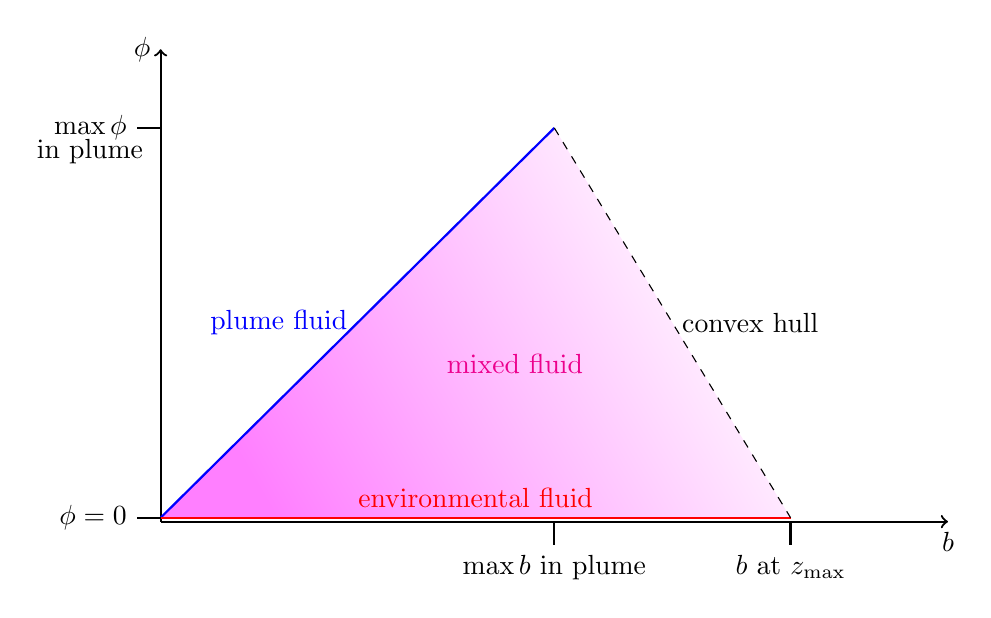
\begin{tikzpicture}
		\draw[thick, ->] (0,0) -- (10, 0) node[below] {$b$};
		\draw[thick, ->] (0,0) -- (0, 6) node[left] {$\phi$};
		\shade[left color = white, right color = magenta, opacity = 0.5, shading angle = -60] 
		(0, 0.05) -- (5, 5) -- (8, 0.05) -- cycle;
		\draw[thick, magenta] (4.5, 2) node {mixed fluid};
		\draw[thick, blue] (0,0.05) -- (5, 5) node[midway, above, left] {plume fluid};
		\draw[thick, red] (0,0.05) -- (8, 0.05) node[midway, above] {environmental fluid};
		\draw[dashed] (5,5) -- (8, 0.05) node[midway, right] {convex hull};
		\draw[thick] (0, 0.05) -- (-0.3, 0.05) node[left] {$\phi = 0$};
		\draw[thick] (8, 0) -- (8, -0.3) node[below] {$b$ at ${z_{\max}}$};
		\draw[thick] (5, 0) -- (5, -0.3) node[below] {$\max b$ in plume};
		\draw[thick] (0, 5) -- (-0.3, 5) node[left] {$\max \phi$};
		\draw (-0.1, 4.7) node[left] {in plume};
	\end{tikzpicture}
	\caption{Schematic diagram of the segregated volume distribution and its physical interpretation.}
	\label{fig:PDFschematic}
\end{figure}

As shown in figure~\ref{fig:PDFschematic}, a simple constraint on the largest accessible environmental
buoyancy is the buoyancy at $z_{\max}$ in the initial local stratification.  In fact, the local buoyancy
gradient is modified as the plume pushes environmental fluid upwards, so $\left.b\right|_{z_{\max}}$ is
typically an overestimate for the largest buoyancy accessed via mixing. This constraint is shown as a
vertical dashed line in figure~\ref{fig:modPDF}(b)--(d), evidently an overestimate for this simulation.
The largest buoyancy and tracer concentration at the bottom of the stratified layer is also a maximal
constraint for the source line. This constraint is not indicate in figure~\ref{fig:modPDF} as the maximum
buoyancy and tracer concentration varies in time. 

\begin{figure}
	\centering
	\makebox[\textwidth][c]{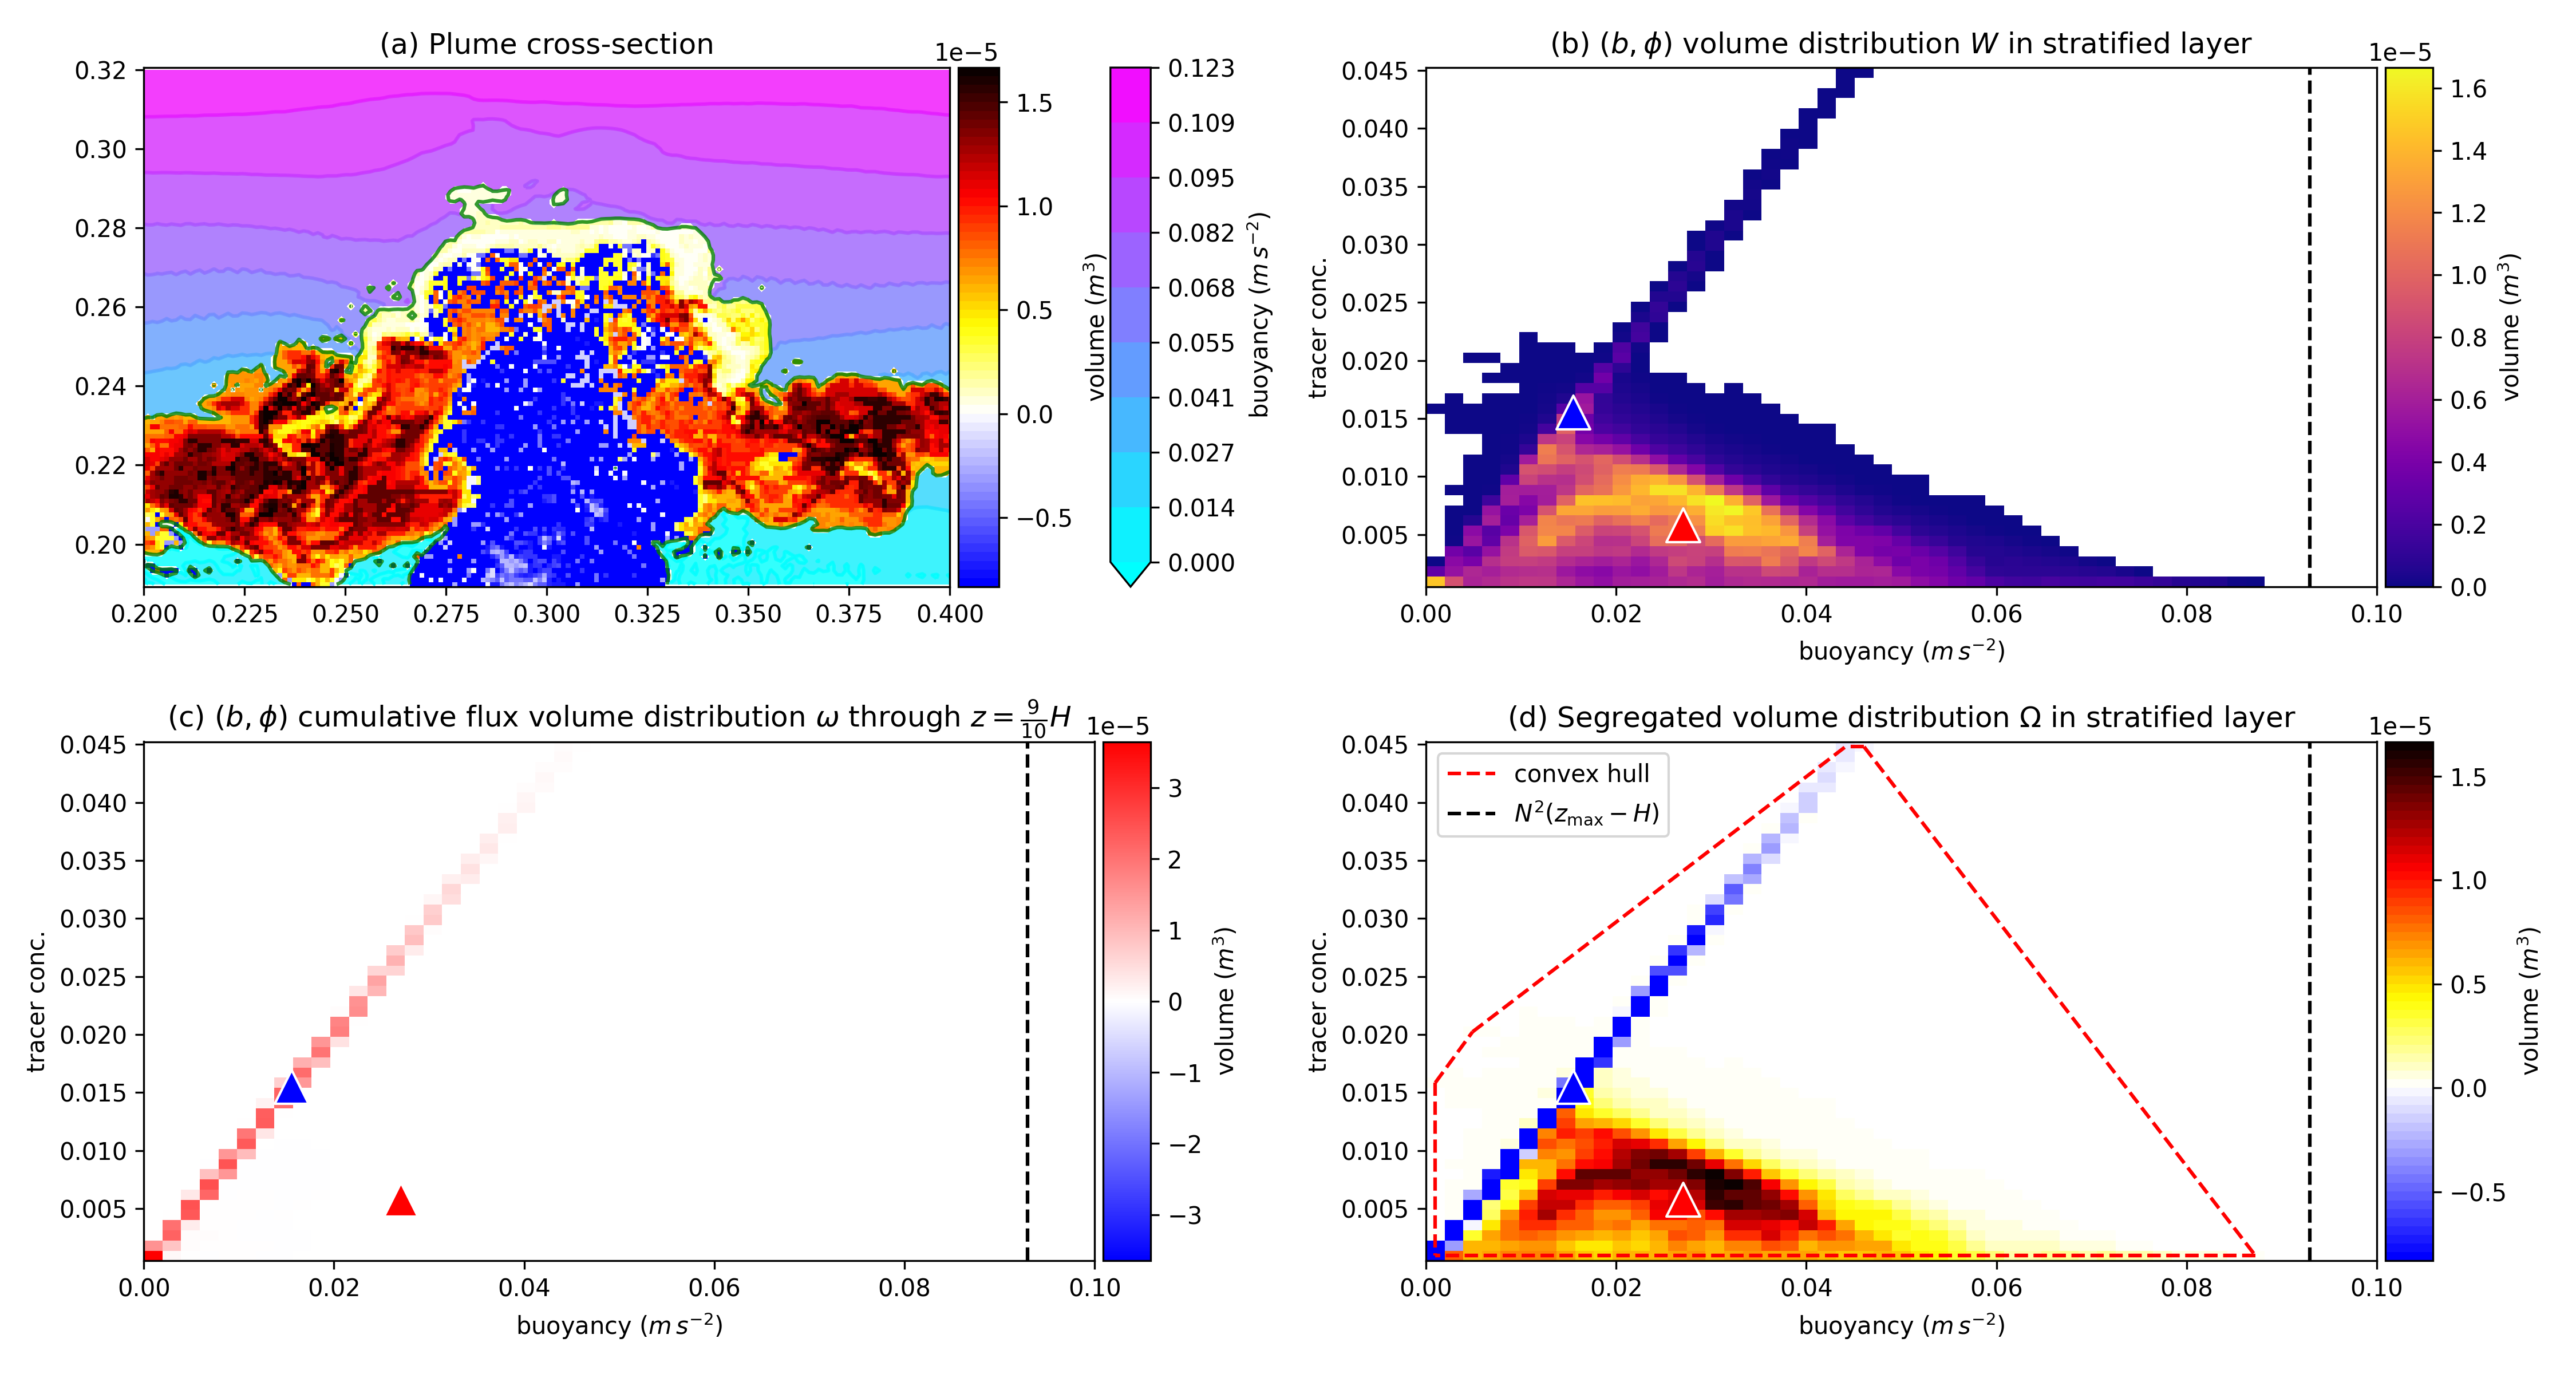
\includegraphics[width=1.2\textwidth]{modifiedPDF}}
	\caption{Composite figure of the construction of the segregated volume distribution with (b) the original
	volume distribution, (c) the cumulative flux volume distribution and (d) the segregated volume
	distribution. Panel (a) shows the plume cross-section with the plume fluid coloured according to the
	corresponding $(b, \phi)$ bin in panel (d).  Data from the same simulation as figure~\ref{fig:jointPDF}.
	The dashed black vertical line in (b)--(d) indicates the initial enviromental buoyancy at $z_{\max}$. The
	red and blue triangles indicate the centre-of-mass of the unmixed plume fluid and the environmentally
	mixed fluid, respectively.}
	\label{fig:modPDF}
\end{figure}

To verify these ideas, it is useful to identify which regions of physical space correspond to
the classes of fluid distinguished by the segregated volume distribution. Figure~\ref{fig:modPDF}(a) shows a
cross-section of the stratified layer in which regions with non-zero tracer concentration are coloured
according to the segregated volume distribution; that is, each point in the physical domain has the colour of
the bin in figure~\ref{fig:modPDF}(d) containing the buoyancy and tracer concentration of that point. Where
the tracer concentration vanishes, the environmental buoyancy is shown. The cross-section supports the
interpretation of the segregated volume distribution as distinguishing plume fluid and environmentally mixed
fluid; the blue, negative volume regions highlight the rising component of the plume. At heights approaching
$z_{\max}$, as the plume begins to overturn and mix with the surrounding environment, the colour suggests
small volumes of fluid at these buoyancies and tracer concentrations, indicative of fluid in the process of
moving from one class of fluid to the other via mixing. In the falling components of the plume either side of
the plume cap, the colour gradually moves to red and black as further mixing homogenises the fluid toward the
buoyancy and tracer concentration found in the large volume of fluid in the spreading intrusion at $z_n$.  

This cross-section view of the corresponding segregated volume distribution is useful for supporting the
physical interpretation of the results, but also for identifying regions of active mixing between plume fluid
and the environment. Evidently most mixing occurs around the overturning plume cap, but there is also evidence
of mixing on the fringes of the central rising column inside the plume. Moreover, we see that the mixing is
not complete after fluid overturns near $z_{\max}$; further environmental fluid is entrained as fluid falls
downwards and joins the intrusion at $z_n$.

\subsubsection{Concentrated mixed region}

\begin{figure}
	\centering
	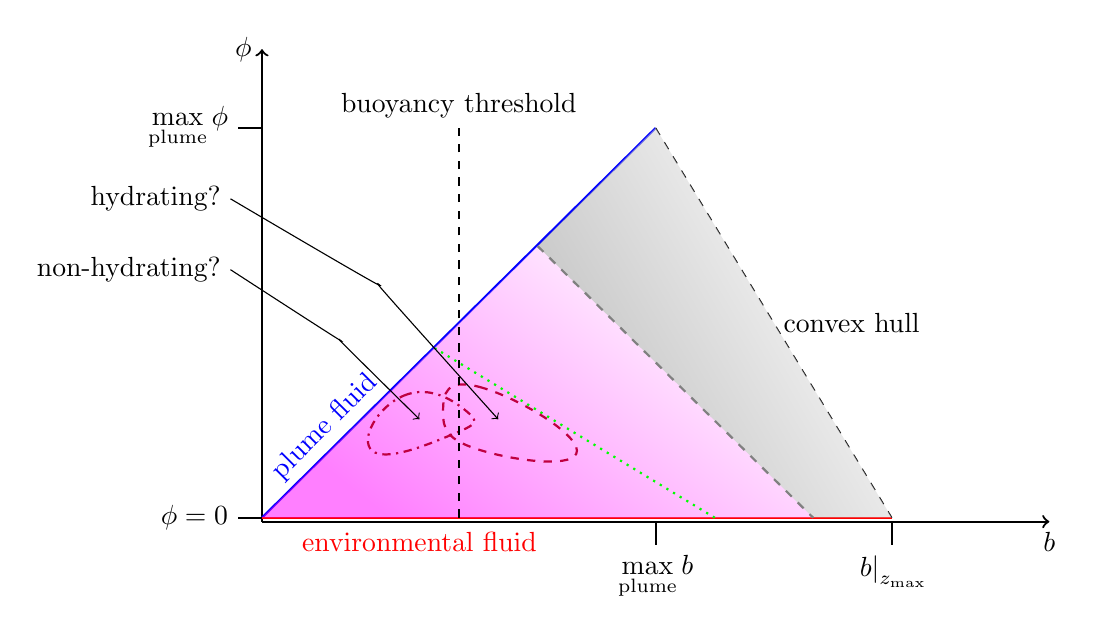
\begin{tikzpicture}{use Hobby shortcut}
		\draw[thick, ->] (0,0) -- (10, 0) node[below] {$b$};
		\draw[thick, ->] (0,0) -- (0, 6) node[left] {$\phi$};
		\draw[thick, blue] (0,0.05) -- (5, 5);
		\draw[thick, blue] (1,1) node[rotate=45, above] {plume fluid};
		\draw[thick, red] (0,0.05) -- (8, 0.05);
		\draw[thick, red] (2, 0) node[below] {environmental fluid};
		\draw[dashed] (5,5) -- (8, 0.05) node[midway, right] {convex hull};
		\draw[thick] (0, 0.05) -- (-0.3, 0.05) node[left] {$\phi = 0$};
		\draw[thick] (8, 0) -- (8, -0.3) node[below] {$\left.b\right|_{z_{\max}}$};
		\draw[thick] (5, 0) -- (5, -0.3) node[below] {$\underset{\text{plume}}{\max} \,b$};
		\draw[thick] (0, 5) -- (-0.3, 5) node[left] {$\underset{\text{plume}}{\max} \,\phi$};

		\shade[left color = white, right color = magenta, opacity = 0.5, shading angle = -38] 
		(0, 0.05) -- (3.5, 3.5) -- (7, 0.05) -- cycle;
		\shade[left color = white, right color = gray, opacity = 0.5, shading angle = -60] 
		(3.5, 3.5) -- (5, 5) -- (8, 0.05) -- (7, 0.05) -- cycle;
		\draw[thick, dashed, gray] (3.5,3.5) -- (7, 0.05);

		\draw[thick, green, dotted] (5.75, 0.05) -- (2.2, 2.2);

		\draw[thick, purple, dashed, smooth cycle] plot[tension=1] coordinates {(4, 0.9) (2.8, 1.7) (2.3, 1.4)
			(2.8, 0.9) };

		\draw[thick, purple, dash dot, smooth cycle] plot[tension=1] coordinates {(1.4, 0.9) (1.8, 1.6) 
			(2.6, 1.4) (2.4, 1.1)};

		\draw (-0.4, 4.1) node[left] {hydrating?};
		\draw (-0.4, 3.2) node[left] {non-hydrating?};

		\draw[smooth, <-] plot[tension=-.1] coordinates{(2, 1.3) (1, 2.3) (-0.4, 3.2)};
		\draw[smooth, <-] plot[tension=-.1] coordinates{(3, 1.3) (1.5, 3) (-0.4, 4.1)};

		\draw[thick, dashed, black] (2.5, 0.05) -- (2.5, 5) node[above] {buoyancy threshold};
	\end{tikzpicture}
	\caption{Schematic diagram of the accessible regions of the volume distribution and the possible
	implications for the stratospheric hydration problem.}
	\label{fig:mixingregions}
\end{figure}

It is evident in figure~\ref{fig:modPDF}(d) that the mixed fluid does not occupy the entire convex hull 
shown in figure~\ref{fig:PDFschematic}, for two reasons. Firstly, the largest values of buoyancy and
tracer concentration in the plume are found in the largest eddies entering the stratified layer. These eddies
must collapse into smaller eddies before viscous diffusion can take place, which occurs as the eddies rise
through the plume. However, as these eddies decay the buoyancy and tracer concentration homogenises with the
surrounding plume fluid. Mixing between fluid parcels with these large values of buoyancy \& tracer
concentration and enviromental fluid is therefore relatively uncommon. Moreover, as mentioned earlier,
the environmental buoyancy of the initial stratification at $z_{\max}$ is an overestimate for the largest
accessible environmental buoyancy due to modification of the local stratification. Significant accumulation of
mixed fluid is therefore excluded from reaching certain parts of the convex hull, as indicated by the grey
area in figure~\ref{fig:mixingregions}. 

The centre-of-mass (CoM) is a useful indicator of the distribution of each class of fluid. The CoM of the
arriving plume fluid (i.e.\ bins with negative volume) is shown as a blue triangle whilst the CoM of the
environmentally mixed fluid is shown as a red triangle in figure~\ref{fig:modPDF}. The pre-mixed CoM is at
much smaller buoyancy and tracer concentration than the largest values found as the plume enters the
stratified region, supporting the earlier argument that most plume fluid mixes internally before mixing with
the environment. The post-mixed CoM also supports the idea that the mixed fluid is generally confined to a
small region of the available convex hull.

Figure~\ref{fig:modPDF}(d) suggests that the bulk of the mixed fluid lies in an even more constrained region,
as indicated by the dotted green line in figure~\ref{fig:mixingregions}; it is exploration of this fact that
ultimately links back to the motivating atmospheric question. Simplistically, one might imagine that after
the transient dynamics of a convective overshoot have settled, the distinction between tracer which remains in
the stratosphere and tracer which settles back into the troposphere is some buoyancy threshold -- see
figure~\ref{fig:mixingregions}. If the mixed fluid is concentrated at buoyancies greater than this threshold,
there is a large irreversible transport of tracer into the stratosphere. If the mixed fluid is concentrated at
lower buoyancies than the threshold, there is only a small irreversible transport even if large tracer
concentrations are transiently present in the stratosphere. Whilst this is a simplistic representation of the
physical processes determining whether tracer remains in the stratosphere, particularly in the case of water
vapour where distinct phases and temperature-dependent saturation of air play a crucial role, it is clear
that we are interested in what sets the distribution of the mixed fluid within the accessible regions of the
segregated volume distribution. Moreover, it is useful to understand what sets the boundaries of this
concentrated region, and how the location of the concentrated region might depend on and be predicted by bulk
properties of the penetrating plume.

%%%%%%%%%%%%%%%%%%%%%%%%%%%%%%%%%%%%%%%%%%%%%%%%%%%%%%%%%%%%%%%%%%%%%%%%%%%%%%%%%%%%%%%%%%%%%%%%%%%%%%%%%%%%%

\section{Turbulent mixing}
\label{sec:turbmix}
In the preceding section, we focused on methods of analysing the transport of passive tracer as a plume
penetrates a stably stratified layer. In particular, we developed a method of identifying fluid composed of
mixed plume and environmental fluid. In this section, we examine the characteristics of the mixing itself
using a number of well established metrics of mixing activity and energy transfer. We will establish which
metrics are the most useful for understanding the mixing processes involved in convective penetration, and use
the segregated volume distribution method to establish some properties of the environmentally mixed plume fluid.

\subsection{Mixing metrics}
\label{sec:mixing}

In the literature, many different metrics are used to examine mixing and characterise where it is strongest
and which mechanisms are responsible for the mixing. Figure~\ref{fig:mixing} shows a selection of these
metrics, some of which are also useful for analysing the energetics of the problem, for an instantaneous
snapshot of the plume in the stratified region. The time variation of these metrics is also of interest, but
difficult to present clearly. The snapshot displayed here is chosen to be representative.

\begin{figure}
	\centering
	\makebox[\textwidth][c]{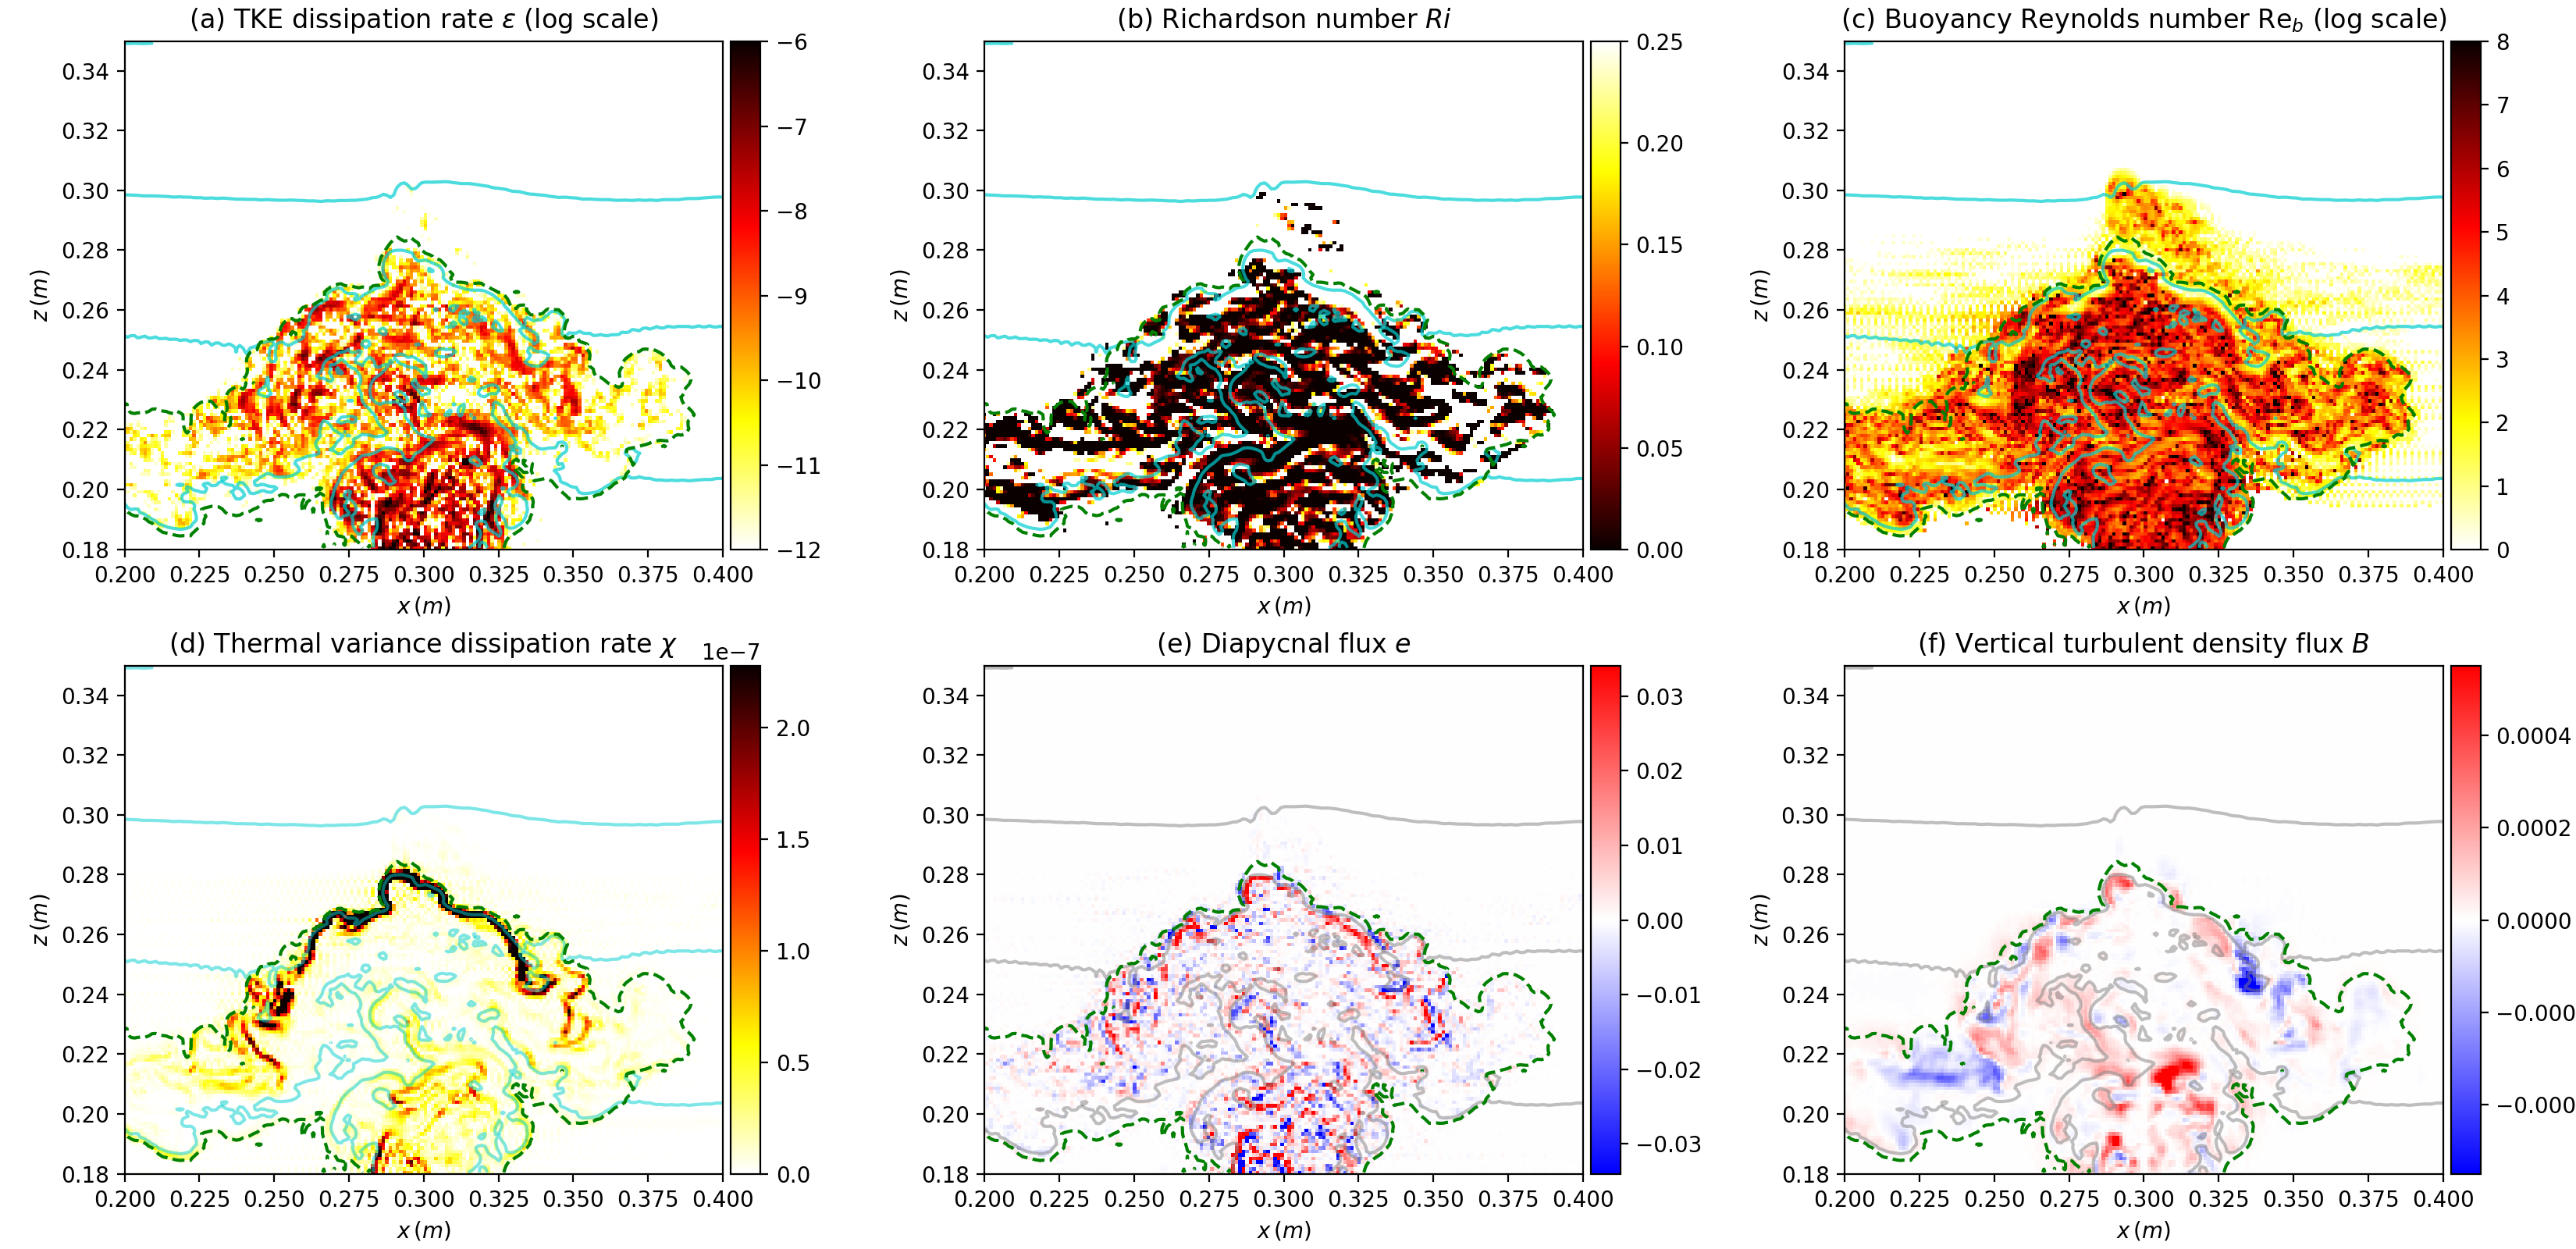
\includegraphics[width=1.1\textwidth]{mixing}}
	\caption{Cross-sections through the plume centreline of the penetration region, showing comparisons of
	mixing metrics at a single time $t = 9 \, s$ in a simulation with the same parameters as in
	figure~\ref{fig:jointPDF}. Green lines are the tracer surfaces $ \phi = 10^{-3}$ and buoyancy contours are
	shown in grey or blue depending on the colourbar used for the metric. }
	\label{fig:mixing}
\end{figure}

\begin{enumerate}[label=(\alph*)]
	\item The \textbf{Turbulent Kinetic Energy (TKE) dissipation rate} $\varepsilon$ represents the conversion
		of kinetic energy into internal energy as a result of turbulent velocity gradients working against
		turbulent deviatoric stresses, defined as
		\begin{equation}
			\varepsilon \equiv 2\nu_{\text{eff}} \overline{\frac{\partial u'_i}{\partial x_j} \frac{\partial
					u'_i}{\partial x_j}}
		\end{equation}
		where $\overline{\cdot}$ represents an appropriate average to isolate the turbulent velocity component
		$\bm{u}' = \bm{u}-\overline{\bm{u}}$. Note that strictly this is the \emph{pseudo-dissipation}, a
		modified version of the dissipation which tends to simplify the form of equations relating to TKE,
		with a factor $\nu \overline{\partial_j u'_i \partial_i u'_j}$ subtracted that is small and introduces
		an error typically around $2\%$. The TKE dissipation rate represents a sink in the TKE evolution
		equation, and is positive definite.  Physically, this represents the fact that the conversion of KE to
		internal energy is irreversible.  Note that the spatially varying effective viscosity
		$\nu_{\text{eff}} = \nu + \nu_T$ is used so that sub-grid-scale contributions are accounted for. Large
		values of $\varepsilon$ imply strong turbulent motion. In figure~\ref{fig:mixing}, $\varepsilon$ is
		shown on a log scale due to the large variation.  It is clear that $\varepsilon$ is concentrated
		within the plume, as expected since strong turbulence is confined to the plume. There is a thin layer
		of small but non-zero $\varepsilon$ around $z \sim 27 \,\mathrm{cm}$ which may be a numerical artefact
		or possibly due to gravity waves (yet to be determined). Otherwise, there is little spatial structure
		to $\varepsilon$ within the plume, although there are slightly larger amplitude variations in the
		centre of the plume and the overturning plume cap compared with the spreading intrusion.

	\item The \textbf{Richardson number} $\mathrm{Ri}$ is a dimensionless number representing the balance
		between buoyant and shear forces. It is defined differently depending on the context, for example
		$\Gamma$ defined earlier. Here we consider the \emph{local gradient} Richardson number, defined as
		\begin{equation}
			\mathrm{Ri} \equiv \frac{2\frac{\partial b}{\partial z}}{\left(\frac{\partial u}{\partial
			z}\right)^2 + \left(\frac{\partial v}{\partial z}\right)^2}
			\label{eq:rich2}
		\end{equation}
		When $\mathrm{Ri} > \frac{1}{4}$, buoyancy tends to suppress shear-driven turbulence and the
		associated diapycnal transport is restricted towards molecular diffusion only, though other sources of
		turbulence may still provide diapycnal transport. When $\mathrm{Ri} < \frac{1}{4}$, buoyancy cannot
		suppress shear-driven turbulence and shear instabilities can develop, leading to mixing
		\citep{ivey2008}. In figure~\ref{fig:mixing}, dark colours indicate susceptibility to shear
		instability, which is confined to the plume as expected since the surrounding region is stably
		stratified and quiescent. There is a distinct layering of the unstable regions, the lengthscale of
		which may be related to the volume-averaged vertical Taylor scale
		\begin{equation}
			l_z^2 = \frac{\langle u^2 + v^2 \rangle}{\langle \left(\frac{\partial u}{\partial z}\right)^2 +
		\left(\frac{\partial v}{\partial z}\right)^2 \rangle}
		\end{equation}
		where $\langle \cdot \rangle$ denotes a volume average \citep{riley2003}. This scale may be related to
		the \emph{volume-averaged} Richardson number $\mathrm{Ri}_V$, defined as in \eqref{eq:rich2} but with
		$N^2$ replacing $\partial_z b$, via a vertical Froude number
		\begin{equation}
			\mathrm{Fr}_l = \frac{2\pi u'_H}{N l_z} = \frac{2\pi}{\sqrt{2\mathrm{Ri}_V}}
		\end{equation}
		where $u'_H = \langle u^2 \rangle^{1/2} = \langle v^2 \rangle^{1/2}$ is the horizontal root mean
		square velocity. There is also an unstable region slightly above the tracer and buoyancy contours
		which are closely aligned in that region, indicating possible mixing and diapycnal transport of tracer
		as a result. These aspects require further investigation.

	\item The \textbf{buoyancy Reynolds number} $\mathrm{Re}_b$ is another dimensionless quantity used to
		characterise turbulent mixing in stratified flows, defined as
		\begin{equation}
			\mathrm{Re}_b \equiv \frac{\varepsilon}{\nu \frac{\partial b}{\partial z}}
		\end{equation}
		$\mathrm{Re}_b$ is generally used in oceanographic contexts in combination with the Froude number, and
		it is generally suggested that active turbulence is only present when $\mathrm{Re}_b > 20$
		\citep{garcia2011}, though this does not necessarily hold in an atmospheric context. As for
		$\varepsilon$, a log scale is used due to the wide range of values. In figure~\ref{fig:mixing} the
		most energetic motions are, as expected, confined to the plume. In most of the plume, there is no
		clear spatial structure, though there are several relatively less energetic layers which coincide with
		relatively stable layers in the $\mathrm{Ri}$ plot. This suggests there is a strong buoyancy gradient
		in these layers, suppressing turbulence. Note the large amplitudes in the rising part of the plume
		indicating energy-containing large eddies. There are also relatively energetic motions
		outside of the tracer contours at the top of the plume cap, indicating possible turbulence which acts
		to mix the plume fluid with the surroundings.

	\item The \textbf{buoyancy variance dissipation rate} $\chi$ represents irreversible mixing via diffusion,
		defined as
		\begin{equation}
			\chi \equiv \kappa_{\text{eff}} \overline{\left| \nabla b' \right|^2}
		\end{equation}
		where $\kappa_{\text{eff}} = \kappa_b + \kappa_{b,T}$ is the effective diffusivity of buoyancy,
		accounting for sub-grid-scale contributions as with the effective viscosity. Large values of $\chi$
		imply strong diffusive mixing and a smoothing of the buoyancy gradient as a result. In
		figure~\ref{fig:mixing} we find the strongest diffusive mixing occurring at the top of the plume, as
		expected since this region has the strongest buoyancy gradients. Other regions of strong mixing are in
		the subsiding regions near the plume top, as more buoyant environmental fluid is pulled down
		introducing strong buoyancy gradients.

	\item \textbf{Vertical turbulent buoyancy flux} $B$ measures the net upwards transport of buoyancy by
		turbulence, representing the conversion of kinetic energy (KE) into potential energy (PE) when $B > 0$
		as relatively heavy fluid is moved upwards, and vice versa when $B<0$. Here, we define
		\begin{equation}
			B = \overline{b'w'}
		\end{equation}
		where $b'$ and $w'$ are the turbulent components, calculated as the anomaly from the 
		azimuthally averaged buoyancy and vertical velocity. In future work, this could be modified to account
		for both spatial and temporal covariance as in section~\ref{sec:setup}. In figure~\ref{fig:mixing} we
		generally find $B > 0$ in the rising component of the plume and $B < 0$ in falling components of the
		plume. Physically this indicates that turbulence in the plume gradually converts KE into PE as the
		plume rise slows.  Once the plume fluid overturns, the stored PE is then converted back to KE.
		Relatively little energy conversion is seen in the spreading intrusion. At the top edges of the plume,
		there is some conversion of KE to PE, further indicating mixing.

	\item The \textbf{diapycnal flux} is the normal flux across an isopycnal surface, sometimes referred to as
		the diapycnal entrainment velocity $e$. We have
		\begin{equation}
			e = w - \frac{\partial z}{\partial \tilde{t}} - u\frac{\partial z}{\partial\tilde{x}} -
			v\frac{\partial z}{\partial\tilde{y}}
		\end{equation}
		where $\tilde{\cdot}$ indicates the calculation of partial derivatives with $\rho$ (or equivalently $b$)
		fixed, i.e.\ on isopycnal surfaces \citep{deszoeke1993}. It may be shown that
		\begin{equation}
			e = \frac{\partial z}{\partial b}\frac{\mathrm{D}b}{\mathrm{D}t} = \kappa_{eff} \frac{\partial
				z}{\partial b}\nabla^2 b
		\end{equation}
		where, for the purposes of reducing noise, we use $\frac{\partial z}{\partial b} \approx N^{-2}$ as a
		global average. Positive values of $e$ represent the transport of fluid to greater buoyancy and the
		opposite for $e < 0$. In figure~\ref{fig:mixing} the spatial structure is not clear, though confined
		to the plume as expected. There are large amplitude variations in the bottom centre of the plume as
		large eddies travel upwards and entrain fluid. Large positive values are found at the top, overturning
		part of the plume, further supporting the implication of diapycnal transport found in plots of
		$\mathrm{Ri}$, $\varepsilon$ and $\chi$. Similarly, in the subsiding component of the plume there is
		negative $e$ as a result of more buoyant environmental fluid mixing with less buoyant plume
		fluid.

\end{enumerate}

Some of these definitions use the squared buoyancy frequency $N^2 = \left.\frac{\partial b}{\partial
z}\right|_{t=0}$ as a measure of the buoyancy gradient in the literature. However, in the region of interest,
the buoyancy gradient is heavily modified by the impinging plume, in which case the dynamical gradient
$\partial_z b$ may be a more useful measure of the local buoyancy gradients. In figure~\ref{fig:mixing}, the
local buoyancy gradient is used in $\mathrm{Ri}$ as turbulent shear instabilities depend on the strength of
the \emph{local} shear. Similar, the local buoyancy gradient is used in $\mathrm{Re}_b$ to indicate energetic
motions acting to strengthen the buoyancy gradient. 

\subsection{Properties of pre- and post-mixed fluid}
To investigate the metrics of turbulent mixing further, we investigate their values when distinguishing
between plume fluid and environmentally mixed fluid, using the segregated volume distribution method. In this
way, we verify the ideas established thus far on the physical interpretation of the two classes of fluid
highlighted in the segregated volume distribution, and work towards understanding the mixing mechanisms
involved.

\begin{figure}
	\centering
	\makebox[\textwidth][c]{
		\begin{subfigure}[c]{0.6\textwidth}
			\centering
			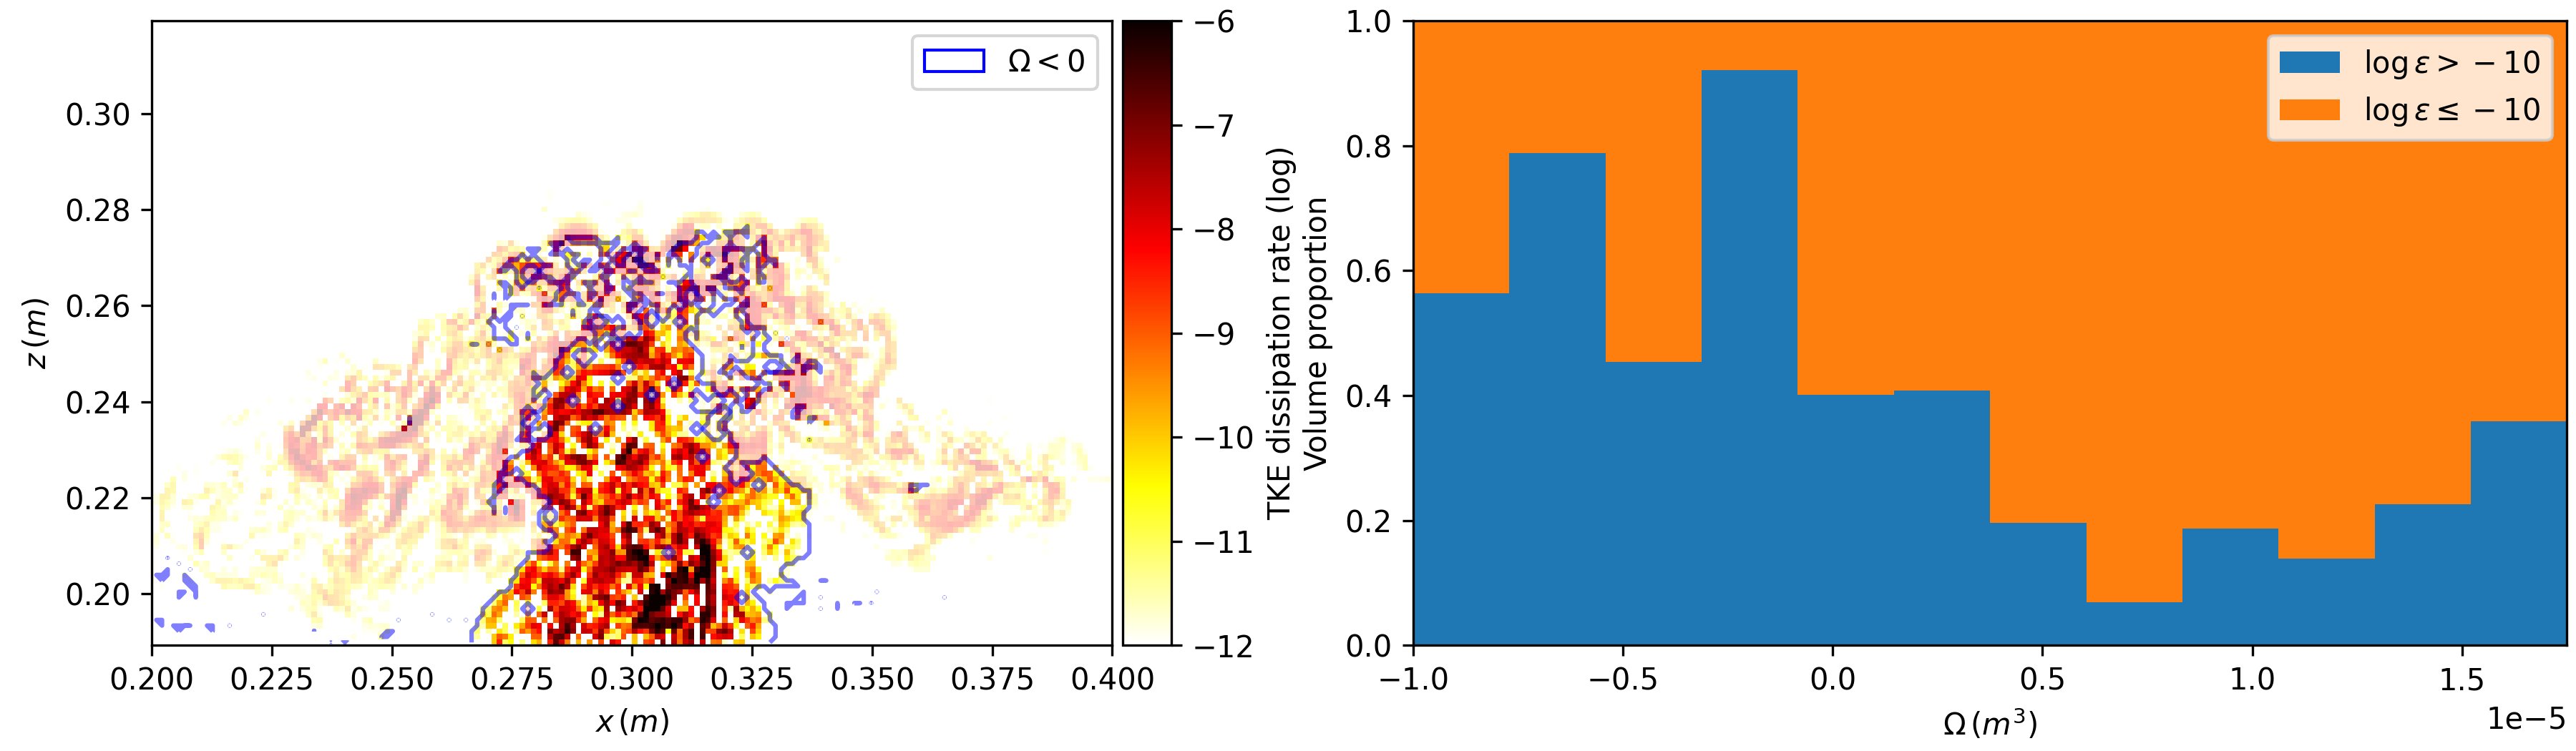
\includegraphics[width=\textwidth]{eps_vol}
			\caption{Turbulent kinetic energy dissipation rate $\varepsilon$. Log scale used in right panel.
			Threshold $\log \varepsilon > -10$.}
			\label{fig:eps_vol}
		\end{subfigure}
		\hspace{1em}
		\begin{subfigure}[c]{0.6\textwidth}
			\centering
			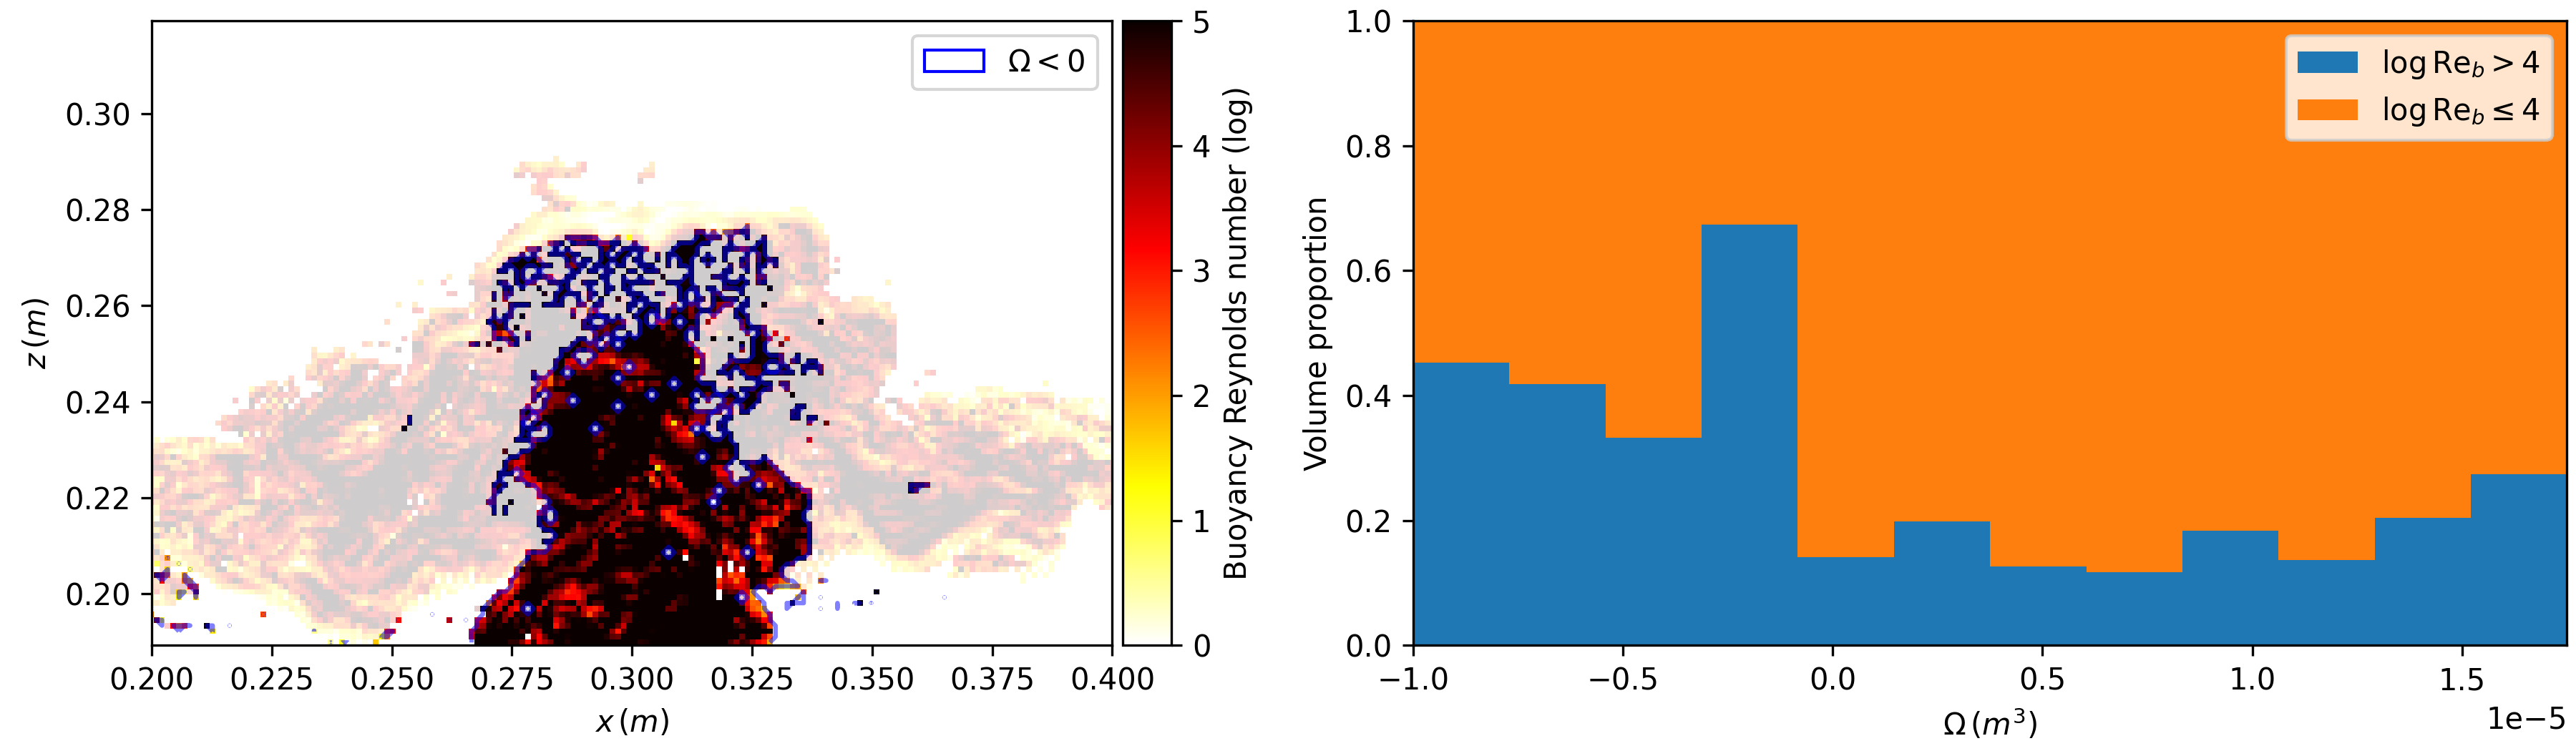
\includegraphics[width=\textwidth]{Re_b_vol}
			\caption{Buoyancy Reynolds number $\mathrm{Re}_b$. Log scale used in right panel. Threshold $\log
			\mathrm{Re}_b > 4$.}
			\label{fig:Re_b_vol}
		\end{subfigure}
	}\\
	\vskip\baselineskip
	\makebox[\textwidth][c]{
		\begin{subfigure}[c]{0.6\textwidth}
			\centering
			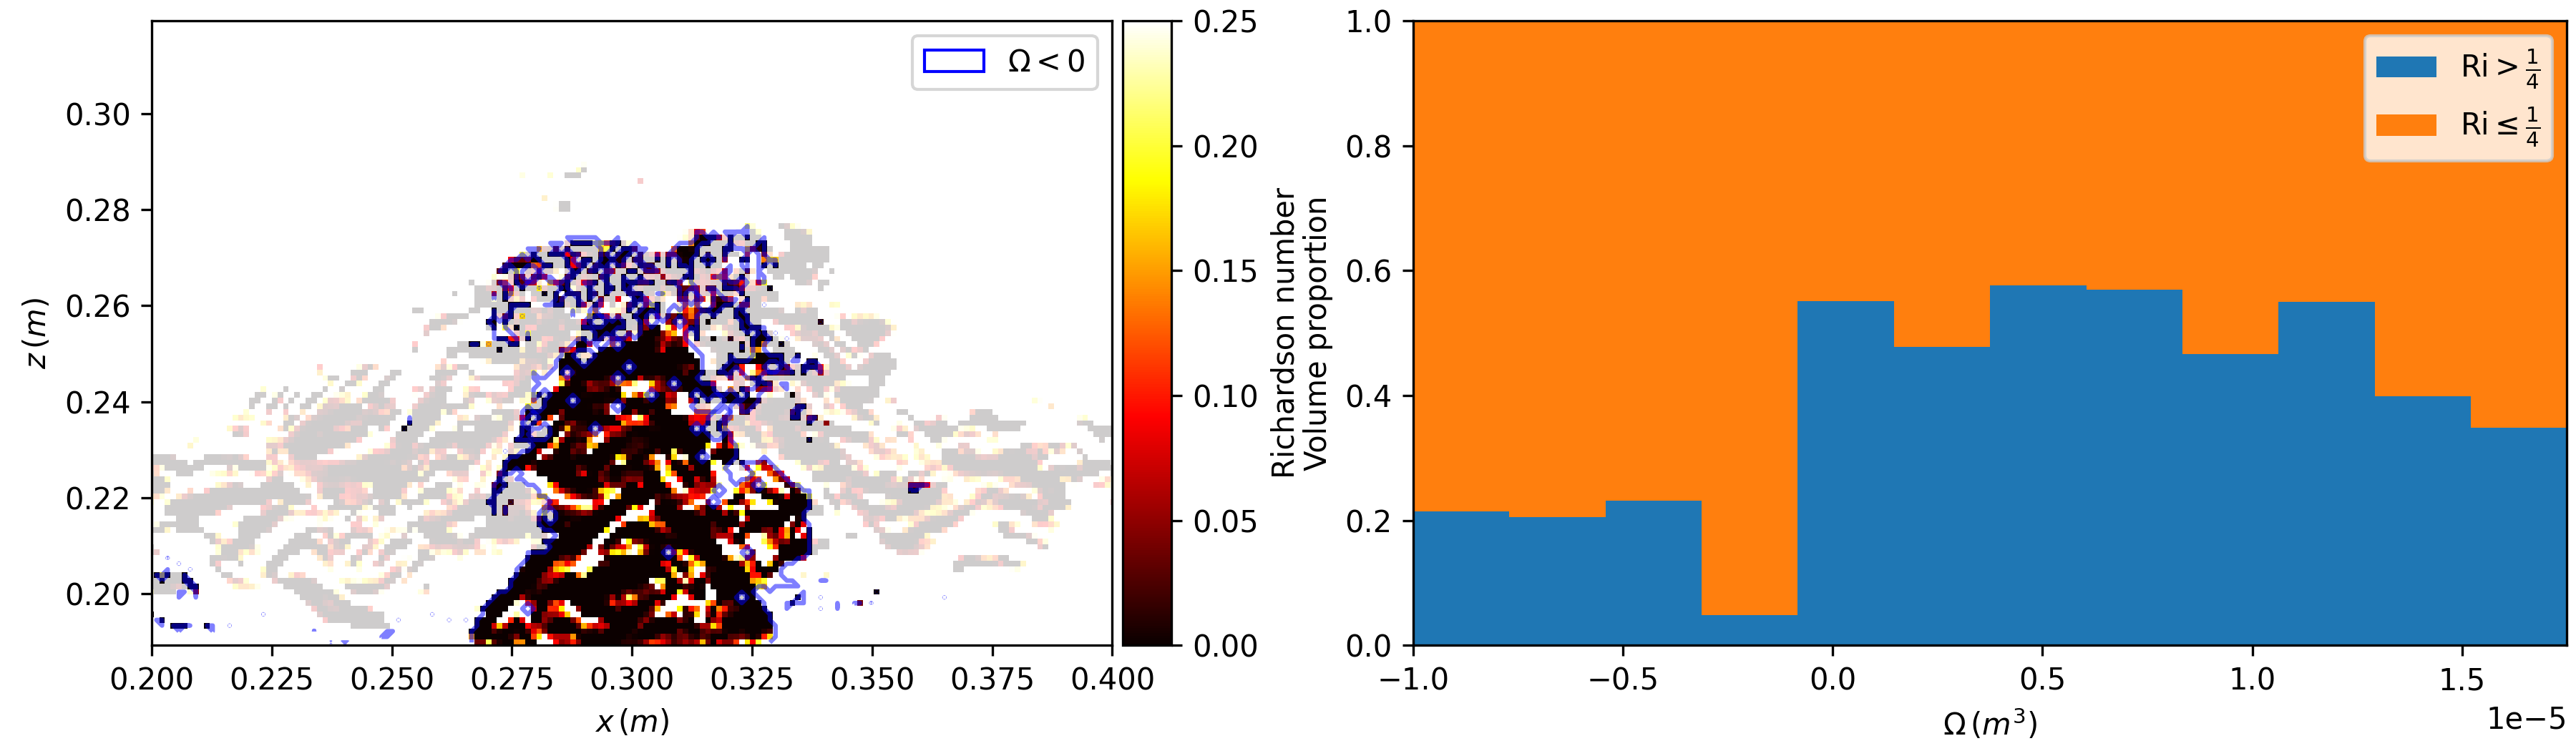
\includegraphics[width=\textwidth]{Ri_vol}
			\caption{Richardson number $\mathrm{Ri}$. Threshold $\mathrm{Ri} > \frac{1}{4}$.}
			\label{fig:Ri_vol}
		\end{subfigure}
		\hspace{1em}
		\begin{subfigure}[c]{0.6\textwidth}
			\centering
			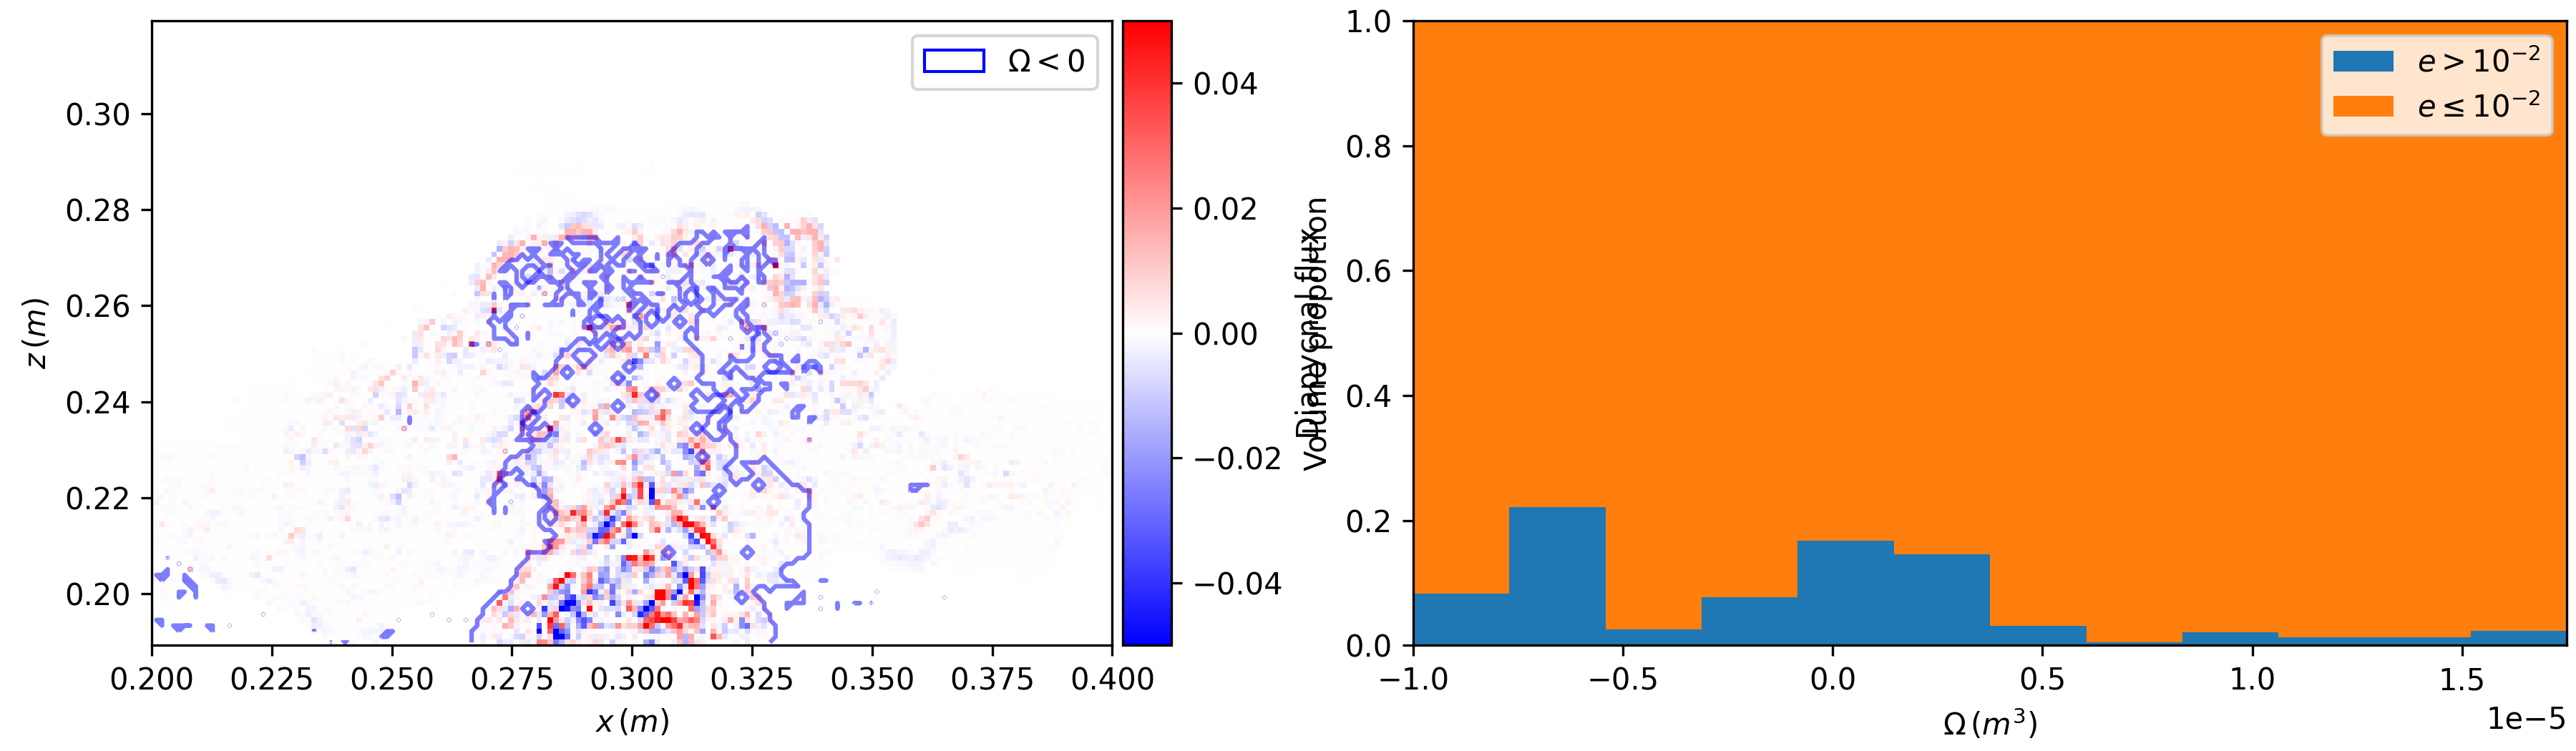
\includegraphics[width=\textwidth]{e_vol}
			\caption{Diapycnal flux $e$. Threshold $e > 10^{-2}$.}
			\label{fig:e_vol}
		\end{subfigure}
	}
	\caption{Volume proportion plots of a selection of mixing metrics discussed in section~\ref{sec:mixing}
	(left). Plume cross-sections showing the relevant metric and unmixed plume regions
	with $\Omega < 0$ highlighted (right).}
\end{figure}

In this section we will examine the mixing characteristics as follows. The range of volume represented in the
segregated volume distribution (see figure~\ref{fig:modPDF}) is separated into equal sized bins. Given a range
of volume $\Omega$, we identify the fluid in the stratified layer with buoyancy and tracer concentration
corresponding to values of $\Omega$ lying in that range. We then compute the proportion of this fluid with
some metric exceeding a threshold set based on figure~\ref{fig:mixing}. Repeating for all bins, we form a 2D
plot with segregated volume distribution weight $\Omega$ on the horizontal axis and the proportion on the
vertical axis. The threshold is chosen to identify particular properties: for example, when considering the
diapycnal flux $e$ we choose a threshold $10^{-2}$ so that we can distinguish fluid where tracer is being
transported to greater buoyancies. Alongside the volume proportion plot we also show a cross-section of the
relevant field. Regions of the plume with corresponding segregated volume distribution weight $\Omega < 0$ are
highlighted to distinguish parts of the plume not yet mixed with the environment, to aid interpretation of the
results.

\begin{enumerate}[label=(\alph*)]
	\item Figure~\ref{fig:eps_vol} shows the volume proportion plot for the TKE dissipation rate $\varepsilon$
		using a log-scale and a threshold $\log \varepsilon > -10$, indicating strong turbulent motion. We
		find that large proportions of unmixed plume fluid exhibit turbulent motion, as expected in the rising
		plume. Moreover, there is also a large proportion of turbulent fluid in regions with $\Omega \approx
		0$, interpreted as regions where active mixing is occuring. The plume cross-section demonstrates that
		the values of $\varepsilon$ found within the environmentally mixed fluid are smaller, in particular
		within the spreading intrusion. In the subsiding fluid around the plume cap, strong turbulent motion
		is still present.

	\item The buoyancy Reynolds number $\mathrm{Re}_b$ indicates energetic motion where it is large. The
		choice of threshold is based on figure~\ref{fig:mixing}, since what constitutes an energetic motion is
		relative and depends on the system. We choose $\log \mathrm{Re}_b > 5$ as the threshold. The volume
		proportion plot in figure~\ref{fig:Re_b_vol} indicates that the most energetic motions lie within the
		rising plume, with a lower proportion of energetic motions in fluid with $\Omega \gtrapprox 0$. The
		plume cross-section suggests that in the spreading intrusion, $\mathrm{Re}_b$ reaches similar maxima
		to within the rising plume, but there are also more regions within the intrusion with smaller
		$\mathrm{Re}_b$.

	\item The volume proportion plot for the Richardson number $\mathrm{Ri}$ is shown in
		figure~\ref{fig:Ri_vol}. The natural choice of threshold is $\mathrm{Ri} > \frac{1}{4}$, which
		indicates regions in which buoyancy tends to inhibit shear instability. We find that unmixed plume
		fluid $\Omega < 0$ is dominated by regions with $\mathrm{Ri} \le \frac{1}{4}$, suggesting
		a susceptibility for shear instability to arise. In regions with mixed environmental and plume fluid,
		the proportion is more even between regions with buoyancy dominating and regions with shear
		dominating. This observation is supported by the plume cross-section.

	\item Figure~\ref{fig:e_vol} shows the volume proportion plot for the diapycnal flux $e$. Here, we examine
		regions where tracer is transported up-gradient across buoyancy surfaces by choosing the threshold $e
		> 10^{-2}$. There are two groups of $\Omega$ with non-trivial volume proportion of fluid with $e >
		10^{-2}$. First, in support of our earlier conclusions on the physical interpretation of fluid with
		$\Omega \approx 0$, we find up-gradient transport of tracer, indicating active mixing. Similarly we
		find active mixing in regions with $\Omega < 0$, as expected as the turbulent motions mix tracer in
		the rising plume.
\end{enumerate}

Finally, we consider the volume proportion plot for the buoyancy variance dissipation rate $\chi$. This is
arguably the best indicator of active mixing, as it signifies intense buoyancy gradients which supports
strong diffusion. Combined with active turbulent motion which acts to stretch isoscalar surfaces,
significant transport of tracer across buoyancy surfaces is possible. As with the buoyancy Reynolds number,
the choice of threshold is somewhat arbitrary and guided by figure~\ref{fig:mixing}; we choose $\chi >
10^{-7}$ to distinguish intense buoyancy gradients. Alongside the volume proportion plot in
figure~\ref{fig:chi_vol}, we show a cross-section of the plume coloured according to the segregated volume distribution
(as in figure~\ref{fig:modPDF}(a)) with the regions with $\chi > 10^{-7}$ highlighted. We find that other than
in the rising plume in which sharp buoyancy gradients occur within large eddies, the main region with intense
buoyancy gradients is at the edge of the overturning plume cap and the subsiding regions surrounding it. In
section~\ref{sec:segjointPDF} we identified this region as predominantly composed of fluid with $\Omega
\approx 0$, indicating fluid in the process of mixing with the environment. This is supported by the volume
proportion plot, with the greatest proportions of fluid with $\chi > 10^{-7}$ found where $\Omega \approx 0$.

\begin{figure}
	\centering
	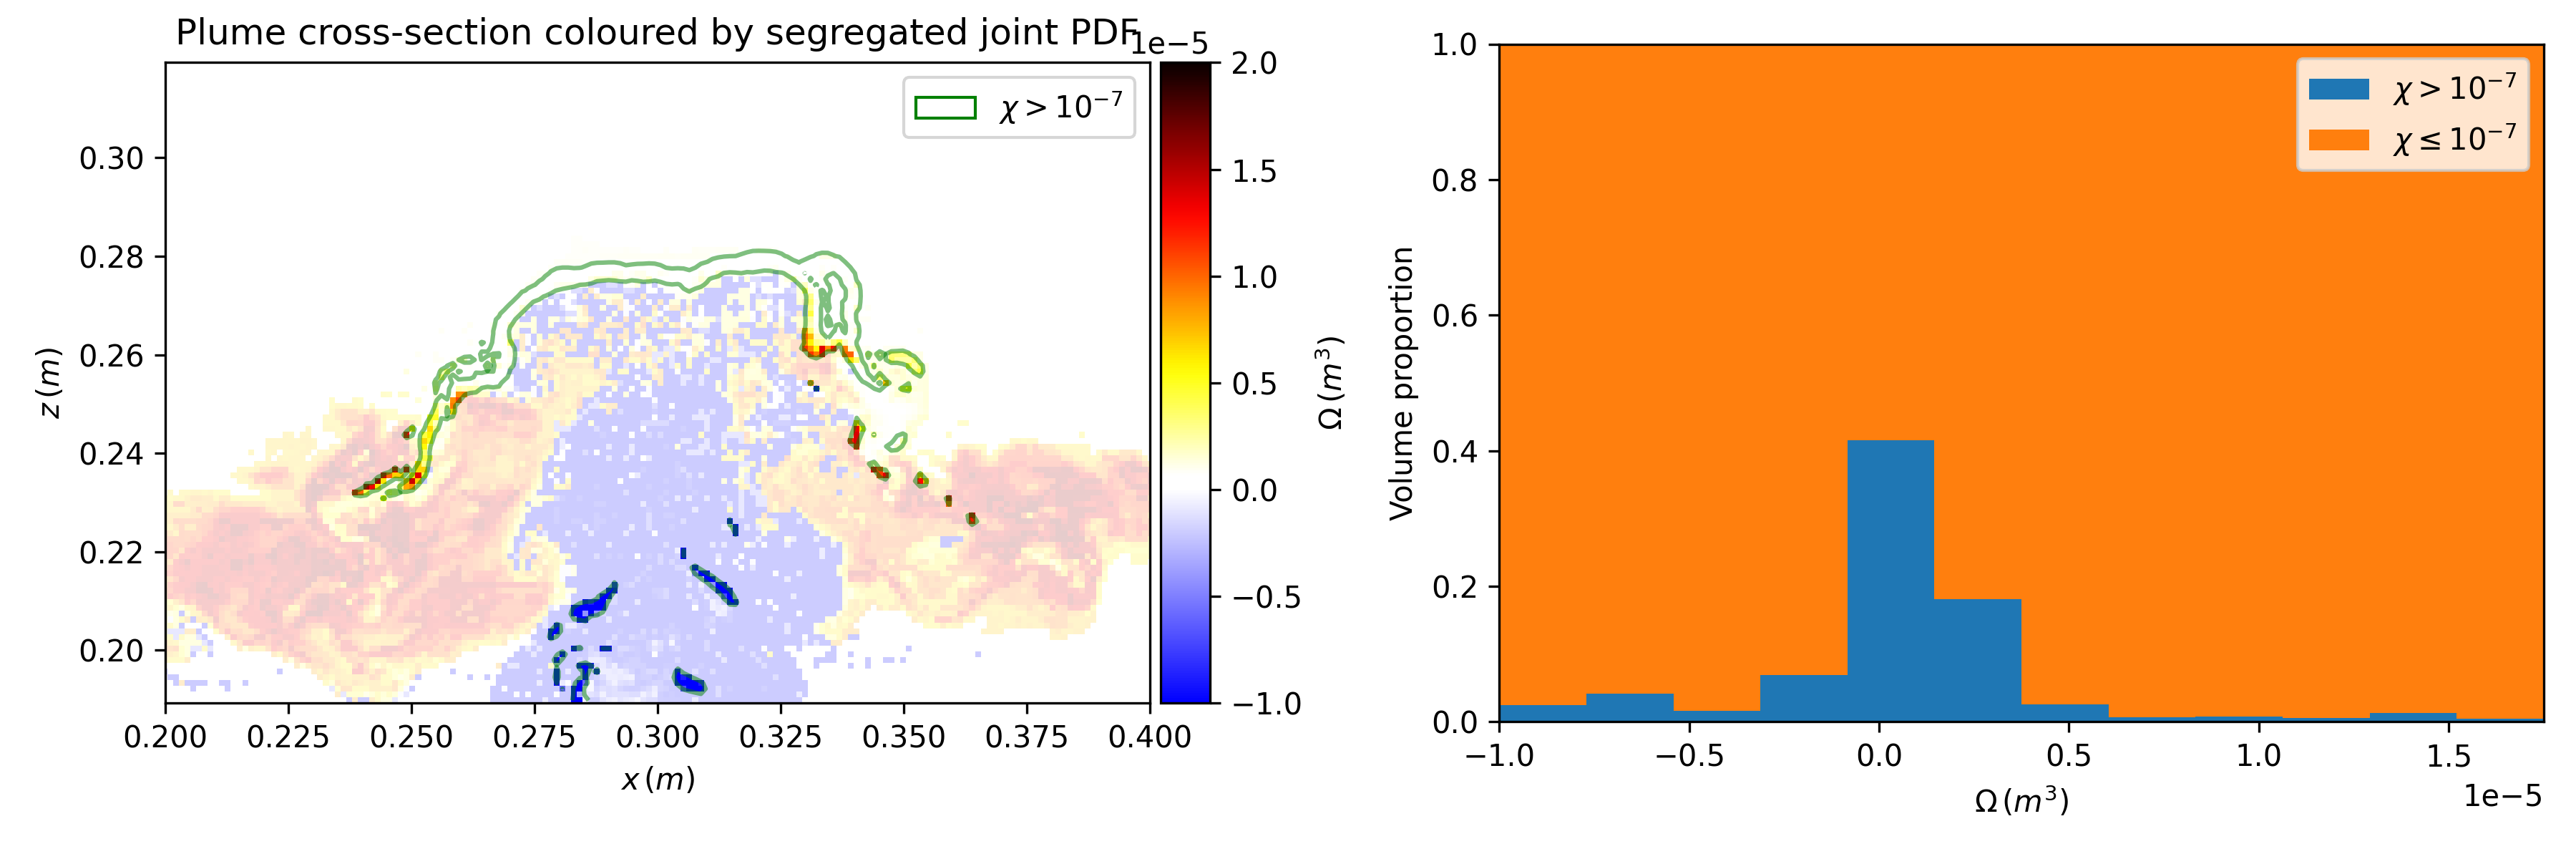
\includegraphics[width=0.8\textwidth]{chi_vol}
	\caption{Volume proportion plot for buoyancy variance dissipation rate $\chi$ with threshold $\chi >
		10^{-7}$ (left). Plume cross-section coloured according to segregated volume distribution with large $\chi$
		region highlighted (right).}
	\label{fig:chi_vol}
\end{figure}

Together, these results help to characterise the fluid in distinct regions of the plume. Broadly, we can
consider three regions: the rising plume, which has not mixed with the environment; the overturning and
subsiding plume cap, which contains fluid actively mixing with the environment; and the spreading intrusion.
In the rising plume, the results discussed here imply there is strong turbulent and energetic motion which
dominates buoyancy and allows shear instabilities to break down and homogenise large eddies, resulting in
strong diapycnal fluxes. There are regions of strong buoyancy gradients, but these quickly decay as the plume
rises and mixes internally. As the rising plume reaches $z_{\max}$, mixing between the plume and the
environment occurs as the fluid overturns and begins to subside. In this region we find strong buoyancy
gradients with strong turbulence persisting in the rising fluid. Compared to the rising component, motions are
less energetic as large amounts of kinetic energy have been converted to potential energy which is then
released as fluid subsides. Whilst the shear is weaker in this region and shear instabilities are better
suppressed than in the rising plume, the strong buoyancy gradients result in strong diapycnal fluxes.
Finally, in the spreading intrusion, we find less energetic motion and weaker turbulence, with weaker
diapycnal fluxes as a result.

%%%%%%%%%%%%%%%%%%%%%%%%%%%%%%%%%%%%%%%%%%%%%%%%%%%%%%%%%%%%%%%%%%%%%%%%%%%%%%%%%%%%%%%%%%%%%%%%%%%%%%%%%%%%%

\section{Future work}

Before concluding the research presented in this essay, we discuss possible routes for future study. The
analysis developed so far has been applied to simulations with a single set of parameters, to gain an
understanding of the phenomenology of the problem, the mixing characteristics present, and the tracer
transport taking place. The natural progression is then to compare these results when one parameter is
varied; the changes indicate which aspects of the problem are dependent on which parameters. For example,
understanding gained may offer a route to deriving scalings for the size and location of the concentrated
region of tracer in the segregated volume distribution. In the context of the motivating atmospheric problem,
there are many other aspects of convective penetration which may aid in understanding hydration of the
lower stratosphere. Here, we discuss two topics which formalise ideas already discussed. 

\subsection{Diapycnal flux}

\label{sec:diapyc}
The diapycnal flux is a key property to understand, as ultimately to answer the question of `how much tracer
makes it to a given height?' it is valuable to instead answer `how much tracer makes it to a given isopycnal
surface?', in which case, the cumulative diapycnal flux goes some way to answering that question. Furthermore,
in the atmospheric context, the diapycnal flux holds even more prominence since the key process for retaining
water vapour in the stratosphere is thought to be the formation of a vapour-rich pocket of air above deep
convection which may then be entrained via the distortion of isentropic (constant potential temperature)
surfaces by shear-induced turbulence \citep{dauhut2018}. It is therefore essential to understand how much
tracer can reach each isentropic surface -- or isentrope -- indicating whether a vapour-rich pocket may form.

The diapycnal flux $e$ discussed in section~\ref{sec:mixing} is a \emph{local} and \emph{instantaneous}
measure of the velocity across buoyancy surfaces. Therefore, whilst indicating intense regions of diapycnal
tracer transport, it does not provide information on the buoyancy surfaces across which the transport takes
place. We may have strong tracer transport across buoyancy surfaces which correspond to isentropes lying in
the troposphere but are transiently distorted into the lower stratosphere by a rising convective overshoot. In
that case, the tracer transport is not significant as the restratification process will bring the tracer back
into the troposphere. It is therefore useful to use the $z^*$ formalism, which implicitly accounts for the
restratification process by construction. We can then examine the diapycnal flux of a tracer $\phi$ across
surfaces with $z^*$ corresponding to buoyancies considered part of the stratosphere.

The $z^*$ formalism uses a sorted density (or buoyancy) coordinate $z_*$ following \citet{winters1996},
defined for a given value of density $\rho_*$ by
\begin{equation}
	z_*(\rho_*, t) = \frac{1}{A_d}\int_{\rho(\bm{x},t) \ge \rho_*} \, \mathrm{d}V
\end{equation}
where $A_d$ is the horizontal area of the domain $V$. Note that this may be reformulated with any scalar $\phi$
in place of the scalar density field $\rho$. When using density (or equivalently buoyancy), $z_*$ may be
interpreted as the vertical coordinate after the restratification process is complete. This interpretation
may require modification given our system includes a constant source of buoyancy. Nonetheless, this formalism
can be used to form an evolution equation for the mean value $\langle \phi \rangle_{z_*}$ of tracer $\phi$ on
a $z_*$ surface, which is defined by \citet{penney2020} as
\begin{equation}
	\langle \phi(z_*, t) \rangle_{z_*} = \frac{1}{A_d} \frac{\partial}{\partial z_*} \int_{\rho(\bm{x}, t) \ge
		\rho_*} \phi(\bm{x}, t) \mathrm{d}V
\end{equation}
and evolves according to
\begin{equation}
	\frac{\partial}{\partial t} \langle \phi\rangle_{z_*} = \frac{\partial}{\partial z_*} \left(
	\frac{\kappa_\phi}{\kappa_\rho}K_\rho \frac{\partial \langle \phi \rangle_{z_*}}{\partial z_*} \right)
	+ \frac{\partial}{\partial z_*}\left(\frac{\partial z_*}{\partial \rho_*} \langle (\kappa_\phi \nabla
	\phi' \cdot \nabla \rho - \kappa_\rho \phi' \nabla^2 \rho)\rangle_{z_*}\right)
	\label{eq:penney}
\end{equation}
where $K_\rho$ is the effective diffusivity for density. The concept of effective (or eddy) diffusivity is
useful as a parameterisation of mixing. \citet{penney2020} investigate the importance of the final `eddy' term
of \eqref{eq:penney}, the idea being that if its cumulative effects are small then it can be ignored and we
can use $K_\rho$ as an eddy diffusivity for $\phi$ when modified by the factor $\kappa_\phi/\kappa_\rho$.

In a related manner, \citet{winters1996} define a general turbulent eddy diffusivity $K_\phi$ for tracer
$\phi$ as
\begin{equation}
	K_\phi \equiv -\phi_d \frac{\mathrm{d}z_*}{\mathrm{d}\phi}
	\label{eq:kphi}
\end{equation}
where $\phi_d$ is the diascalar flux
\begin{equation}
	\phi_d = -\kappa_\phi \frac{\mathrm{d}z_*}{\mathrm{d}\phi} \langle \left| \nabla \phi \right|^2
	\rangle_{z_*}
\end{equation}
The quantity $\phi_d$ and the mean tracer $\langle \phi \rangle_{z^*}$ are powerful tools for understanding
diapcynal tracer transport which may be incorporated into the analysis presented in
sections~\ref{sec:tracertransport} and~\ref{sec:turbmix}.

\subsection{Mixing efficiency}
\label{sec:energetics}
\textcolor{red}{Incorporate some ideas from Wykes mixing efficiency stuff too}

In most physical systems, energy is a useful tool for understanding the dynamics. In this essay we have
discussed some aspects of energetics, for example turbulent kinetic energy and the vertical turbulent buoyancy
flux which represents conversion of KE to PE. In flows with a stable stratification, a component known as the
`background potential energy' of the potential energy is not available for conversion to kinetic energy. The
remaining portion, the `available potential energy', is available to do work and may be irreversibly converted
to background potential energy via molecular mixing. The conversion between various forms of energy is
detailed in \citet{winters1995} who present an `energy diagram' with conversion terms between background
potential, available potential, kinetic, external, and internal energy. The energy budget of restratification
is accounted for using the $z^*$ formalism. A crucial aspect of understanding geophysical flows involving
mixing is to quantify the available potential energy available for mixing. 

A concept often used to describe the energetics of mixing is the \textbf{mixing efficiency} $\mathcal{E}$. It
can be defined in different ways depending on the context \citep{gregg2018}. A useful definition which
incorporates the $z_*$ formalism discussed here is
\begin{equation}
	\mathcal{E} = \frac{\text{Change in background potential energy due to mixing}}{\text{Total energy expended}}
\end{equation}
The background potential energy $E_b$ may be defined as the minimum potential energy attainable through an
adiabatic redistribution of $\rho$. Using the concept of $z_*$ defined above as a vertical position in a
redistributed density field $\rho(z_*)$, we may write $E_b$ as
\begin{equation}
	E_b = g \int_V \rho z_*(\bm{x},t)\,\mathrm{d}V
\end{equation}
The total potential energy $E_p$ is a combination of the background potential energy $E_b$ and the
available potential energy $E_a$, the accessible potential energy which could be released in an adiabatic
redistribution from $\rho(\bm{x},t)$ to $\rho(z_*)$. We have
\begin{equation}
	E_a = g \int_V \rho \left(z-z_*(\bm{x},t)\right)\,\mathrm{d}V
\end{equation}
such that the total potential energy $E_p = E_b + E_a$. 

\citet{winters1995} derive evolution equations for these quantities so that changes in PE due to diabatic
mixing and adiabatic processes may be separated. The change in $E_b$ may be expressed as
\begin{equation}
	\frac{\mathrm{d} E_b}{\mathrm{d}t} = -g\oint \psi \bm{u}\cdot \mathrm{d}\bm{S} + \kappa_\rho g \oint z_*
	\nabla \rho \cdot \mathrm{d}\bm{S} + \kappa_\rho g \int_V -\frac{\mathrm{d}z_*}{\mathrm{d}\rho} \left|
	\nabla \rho \right|^2 \,\mathrm{d}V \label{eq:bpe}
\end{equation}
where $\psi = \int^\rho z_*(\hat{\rho}) \, \mathrm{d}\hat{\rho}$. The first and second terms account for
advection and diffusion across the surface $S$ bounding $V$. The third term is of central importance,
accounting for material changes in $\rho$ due to diapycnal mixing, which acts to increase background potential
energy $E_b$. To apply this formulation to convective penetration, an appropriate choice of $V$ must be made.
Since the entrainment in the rising plume is not the focus, a natural choice for $V$ is the stratified region
$z \geq H$. This also conveniently does away with the need for a buoyancy source in the governing equations
and instead an input flux on the bottom boundary accounts for the buoyancy input of the plume. The governing
equation \eqref{eq:bpe} for $E_b$ would need modification to include this additional flux.

In the context of the atmospheric problem, the advantage of using mixing efficiency is a simplistic way to
determine how much hydration we expect from a certain input of energy from a convective overshoot. The mixing
efficiency yields an estimate for the energy expended via mixing and by further understanding the irreversible
tracer transport arising as a result of mixing with some characeristic energy in the lower stratosphere, we
may form a rough (but convenient) estimate for the water vapour transport. Moreover, an investigation of the
energetics of the convective penetration problem as a whole aid in understanding how large-scale atmospheric
models might represent the energy involved in convective overshoots relative to wider thunderstorm complexes.

\section{Conclusion}
	
In this essay, we begun with the problem of quantifying irreversible water vapour transport in the upper
troposphere \& lower stratosphere via convective overshoots from large thunderstorm complexes. To tackle this,
we reduced the complex atmospheric problem to the idealised fluid dynamical representation of a turbulent
plume penetrating a stably stratified layer. Having verified the capability of large eddy simulations to
represent the essential physics of a buoyant plume, we demonstrated that simulations of convective penetration
reliably represent laboratory experiments of the same setup. We then focus on two aspects of convective
penetration: develop methods of analysing the tracer transport taking place and characterising the turbulent
mixing producing this transport. We first introduced a tracer PDF in buoyancy coordinates, before moving to
buoyancy-tracer space and considering a volume distribution of the stratified layer, in which mixing manifests
as relocation of volume within the distribution, representing the homogenisation of the density and tracer
concentration of the corresponding fluid elements. We introduce a segregated volume distribution which
accounts for the continuous input of buoyancy and tracer by the plume, and discuss its interpretation as
distinguishing fluid arriving in the plume from that which has mixed with the surrounding stratified environment.
Moreover, we are able to identify the regions of most intense mixing between the plume and environment. We
then discuss metrics which describe the intensity of mixing, its driving mechanisms and the diapycnal tracer
transport that results. Using the segregated volume distribution, we characterise the properties of the rising
plume, the regions actively mixing environmental and plume fluid, and the spreading intrusion of mixed fluid. 

Beyond comparing changes in our current analyses under varied stratification strength, there are a number of
questions to be considered further. Complicating factors in the atmospheric case which were omitted in
idealising the problem can be re-introduced to determine their effect, some of which relate to the atmospheric
setup, and some to the physical properties of tracers, passive or otherwise. To better emulate the atmospheric
environment, we could introduce a large-scale shear in the stratified layer which can introduce shear-driven
turbulence, or a weak stratification in the lower layer that is currently quiescent. At present, the
background buoyancy profile is simplified and neglects the complex nature of the UTLS in which the
stratification gradually adjusts from tropospheric to larger stratospheric values; losing the distinction
between a stratified and quiescent layer will inevitably alter the penetration process and possibly the
resulting tracer transport. In the atmosphere, one might consider a convective overshoot as originating from a
central plume which forms the main component of a thunderstorm. The surrounding cloud environment is clearly
not quiescent and crucially, water vapour is present. The importance of this observation could be tested by
introducing an ambient source of tracer in the queiscent lower layer, which will be entrained into the plume
and may increase tracer concentrations at the outer edges, but may also reduce buoyancy. Whether the overall
tracer transport is enhanced or not is an interesting question since we have found that the central regions of
the plume which reach $z_{\max}$ tend to mix with the environment most effectively. Finally, to bring us
closer to the stratospheric hydration problem itself, simple representations of the thermodynamics of water
vapour can be incorporated into the simulations. For example, using multiple passive tracers which represents
distinct phases of water can be used to capture the effects of sublimation and saturation.

%%%%%%%%%%%%%%%%%%%%%%%%%%%%%%%%%%%%%%%%%%%%%%%%%%%%%%%%%%%%%%%%%%%%%%%%%%%%%%%%%%%%%%%%%%%%%%%%%%%%%%%%%%%%%

\appendix

\section{Post-processing method for numerical simulations}
\label{app:postprocessing}

The DIABLO solver uses a 3D Cartesian coordinate system, with a horizontally uniform grid with cell widths
$\Delta x = \Delta y$. High resolution simulations produce large amounts of data, so for practical reasons we
reduce the data from 3D coordinates $(x,y,z)$ to 2D axisymmetric cylindrical coordinates $(r,z)$ by
azimuthally averaging, with the plume centreline as the axis $r=0$. To perform an azimuthal average, the 3D
grid is discretised into cylindrical shells with axes aligned with the plume centreline, each with thickness
$\Delta r \equiv \Delta x = \Delta y$.  Denoting each shell as $S_i$ with $i=0,1, \cdots, N_x/2-1$ we have
\begin{equation}
	S_i \equiv \{ (x,y) \mid i\Delta x \le \sqrt{x^2 + y^2} \le (i+1)\Delta x\}
\end{equation}
The azimuthal average of a variable $\chi$ at radius $r$ and height $z$ is then
\begin{equation}
	a(\chi) = \frac{1}{N}\sum_{\text{shell}} \chi_i(r,z)
\end{equation}
where $\{\chi_i(r,z)\}$ are the observations of $\chi$ from the cylindrical shell containing the radius $r$ at
height $z$ and $N$ is the total number of such observations.

The decomposition of the flow into mean and turbulent components requires an appropriate choice of mean. Under
the assumption of statistical steadiness and statistical homogeneity in the azimuthal direction, the observed
values of a variable $\chi$ at fixed $(r,\phi)$ are i.i.d. random variables, with expected value (mean)
estimated by the combined azimuthal and time average. The (total) time average of a sequence of observations
$\chi_i$ with time steps $\Delta t_i$ over total time $t_{\text{run}}$ is
\begin{equation}
	t(\chi) = \frac{1}{t_{\text{run}}} \sum_i \chi_i \Delta t_i
\end{equation}
where $\chi_i$ are observations at a 3D point $(x,y,z)$ or 2D point $(r,z)$ as desired. The mean component
of a variable $\chi$ is then $\overline{\chi} = t(a(\chi)) = a(t(\chi))$ since the two averages commute. Note
that $t$ and $a$ are idempotent. The turbulent component of a variable $\chi$ is composed of two terms;
spatial fluctuation and temporal fluctuation. The spatial fluctuation $a'(\chi) = \chi - a(\chi)$ is the
difference between $\chi$ and its azimuthal average at each point. The temporal fluctuation $t'(\chi) =
a(\chi) - t(a(\chi))$ is the difference between the azimuthal average of $\chi$ and the total mean of $\chi$.
The Reynolds' decomposition of a variable $\chi$ is then
\begin{equation}
	\chi = \overline{\chi} + \chi' \equiv t(a(\chi)) + a'(\chi) + t'(\chi)
\end{equation}
The covariance of two variables $\chi$ and $\psi$ is defined as
\begin{equation}
	\overline{\chi' \psi'} \equiv \overline{\chi\psi} - \overline{\chi}\overline{\psi}
\end{equation}
Using $\chi' = a'(\chi) + t'(\chi)$ and assuming spatial and temporal fluctuations are uncorrelated so that
$\overline{a't'} \equiv 0$ for any variables, then
\begin{equation}
	\overline{\chi' \psi'} = t(a(a'(\chi)a'(\psi))) + t(a(t'(\chi)t'(\psi)))
\end{equation}
where the first term represents spatial covariance and the second term represents temporal covariance.

\section{Limitations of numerical simulations}
\label{app:limitations}

The DIABLO LES of a buoyant plume exhibits a number of limitations. Some of these are limited to the specific
unstratified configuration considered in the first section, in which there is no vertical limit on the plume
evolution. With the introduction of a stratified layer the plume does not reach the top boundary, so the
associated pressure variation and overturning circulation limitations are not present. 

The volumetric forcing method is advantageous compared to a simple buoyancy gradient at the bottom boundary.
The effect of Gibbs ringing may be reduced by controlling the source radius, and `pinching' of the plume where
inflow dominates the diffusive boundary buoyancy flux is reduced; note the `pinching' above the
forcing region in figure~\ref{fig:radius} still present, but significantly improved from early test
simulations with a boundary gradient. Regardless of the simulation setup, the prescribed profiles of $w$
and $b$ are for an unstratified environment, since the forcing region is shallow enough that the effects of
stratification are not felt.

The presence of a buoyancy source but no sink in the domain remains a limitation when stratification is
introduced, as the local ambient stratification will be modified by the buoyancy input. This
places a limitation on the length of time that simulations can be run. Similarly, time limitations arise from
the generation of internal gravity waves and their interference, as well as the radial spreading of any
intrusions. One way to allow an intrusion to spread for longer is to increase the size of the domain. However,
this limits the resolution that can be achieved whilst maintaining practical use of computer resources.
Furthermore, reduced resolution means more small-scale turbulence must be captured by the LES model and as a
result the turbulence characteristics, and therefore the mixing properties of the flow, may become more
sensitive to the choice of model. The vertical size of the domain, and the depth of the unstratified layer,
is limited by the decay of source effects in the plume generation. As seen in figures~\ref{fig:radius},
\ref{fig:entrain} and~\ref{fig:profilecoeff}, the source effects only become negligible around $z/r_0
\gtrapprox 30$, so the unstratified plume generation region must be large enough to allow the plume to become
fully developed before penetrating the stratified layer when introduced. Note that this is sensitive to the
method of initiating turbulence, as other methods may reduce the lengthscale over which source effects decay
and this must be tested in each simulation configuration. Finally, our volumetric forcing method limits the
types of plume which can be simulated, as some inertial forcing is introduced resulting in $\Gamma < 1$. The
forcing profile and the momentum equation coupling strength must be tested in each simulation configuration to
achieve the desired pre-penetration plume dynamics.

%%%%%%%%%%%%%%%%%%%%%%%%%%%%%%%%%%%%%%%%%%%%%%%%%%%%%%%%%%%%%%%%%%%%%%%%%%%%%%%%%%%%%%%%%%%%%%%%%%%%%%%%%%%%%

\begin{multicols}{2}
{\small\bibliography{biblio}}
\end{multicols}

\end{document}
